\documentclass[%
11pt,%
%oneside,%
twoside,%
%twocolumn,%
titlepage,%
%fleqn,%
%a4page,%
german,%
%headsepline%
]{scrartcl}

%\usepackage{fancyhdr}
%\usepackage{scrpage2}
\usepackage{lastpage}
\usepackage{geometry}
\usepackage{graphicx}
\usepackage[utf8]{inputenc}
\usepackage[ngerman]{babel}
\usepackage{lscape}
\usepackage[framemethod=TikZ]{mdframed}
\usepackage[most]{tcolorbox}
\usepackage{mymath}
\usepackage{units}
\usepackage{nicefrac}
%\usepackage{pgf,tikz}
\usepackage{pgf,tikz,pgfplots}
\pgfplotsset{compat=1.14}
\usepackage{mathrsfs}
\usetikzlibrary{arrows}
\usepackage{colortbl}
\usepackage{hhline}
\usepackage{multirow}
\usepackage[extendedchars]{grffile}
\usepackage{caption}
\usepackage{multicol,calc}
\usepackage{blindtext}
\usepackage{pdfpages}
\usepackage{hyperref}
\usepackage{tikz-er2}
\usepackage{framed}
\usetikzlibrary{arrows}
\usetikzlibrary{positioning}
\usetikzlibrary{shadows}
\usepackage{rotating}
\usepackage{xr}
\usepackage{pifont}
\usepackage[scanall]{psfrag} % Strings in Bildern durch LaTeX-Texte ersetzen
\usepackage[xspace]{ellipsis} % bessere \dots
%\usepackage{picins}
\usepackage{calc} % rechnen
\usepackage{lscape} % Querformat
\usepackage{longtable} % mehrseitige Tabellen
\usepackage{tabulary} % Tabellen mit automatischer Spaltenberechnung
\usepackage[defblank]{paralist} % erweiterte Listen

\usepackage{marginnote}
\usepackage{qrcode}
\qrset{height=9ex}


%\usepackage{romannum}
\usepackage{longtable}
\usepackage{listings}
\usepackage{wrapfig}
\usepackage{pst-plot}
\usepackage{pstricks}
\usepackage[symbol]{footmisc}
\usepackage{xr}
\usepackage[ngerman]{varioref}

\newcommand{\ufrac}[2]{\ensuremath{\,\frac{\mathrm{#1}}{\mathrm{#2}}}}
\newcommand{\name}[1]{\textsc{#1}}

\newcommand{\zitat}[1]{\flqq #1\frqq}
\newcommand{\rede}[1]{``#1''}
\newcommand{\begriff}[1]{``#1''}
\newcommand{\quasi}[1]{``#1''}
\newcommand{\begriffinrede}[1]{`#1'}

\newcommand{\result}[1]{\underline{\underline{#1}}}

\clubpenalty=10000 \widowpenalty=10000


% Command, um Tabellen-Spalten anzupassen
\newcommand{\spaltenheight}{\rule{0mm}{3ex}}
\newcommand{\spaltenwidth}{\rule{3cm}{0mm}}
\newcommand{\spaltensep}{\\[1ex]}
%\arrayrulecolor{darkgreen}
\doublerulesepcolor{white}
\definecolor{lightyellow}{rgb}{1,1,0.8}
\definecolor{Gray}{gray}{0.9}

\newenvironment{system}{\begin{displaymath}
  \left| 
    \begin{array}{rcl}}{\end{array} \right| 
\end{displaymath}}

\newlength{\psein}


% Pagestyle/Layout
%\geometry{a4paper , tmargin =2.5cm,	bmargin=3cm, lmargin =2.5cm,	rmargin =2.5cm,	headheight=3em, headsep=1em, footskip=1cm}
\setlength{\parindent}{0pt} \setlength{\parskip}{1em}
%f\"ur TwoSide
%\lehead{\headmark\pagemark}
%\cehead{}
%\rehead{}
%\lohead{}
%\cohead{}
%\rohead{\headmark}
%f\"ur OneSide
%\ihead{}
%\chead{}
%\ohead{}
%\setheadsepline{0.5pt} % Linie zur Begrenzung
%\setfootsepline{0.5pt} % Linie zur Begrenzung
\pagestyle{headings} % gemachte Einstellungen anwenden


\subject{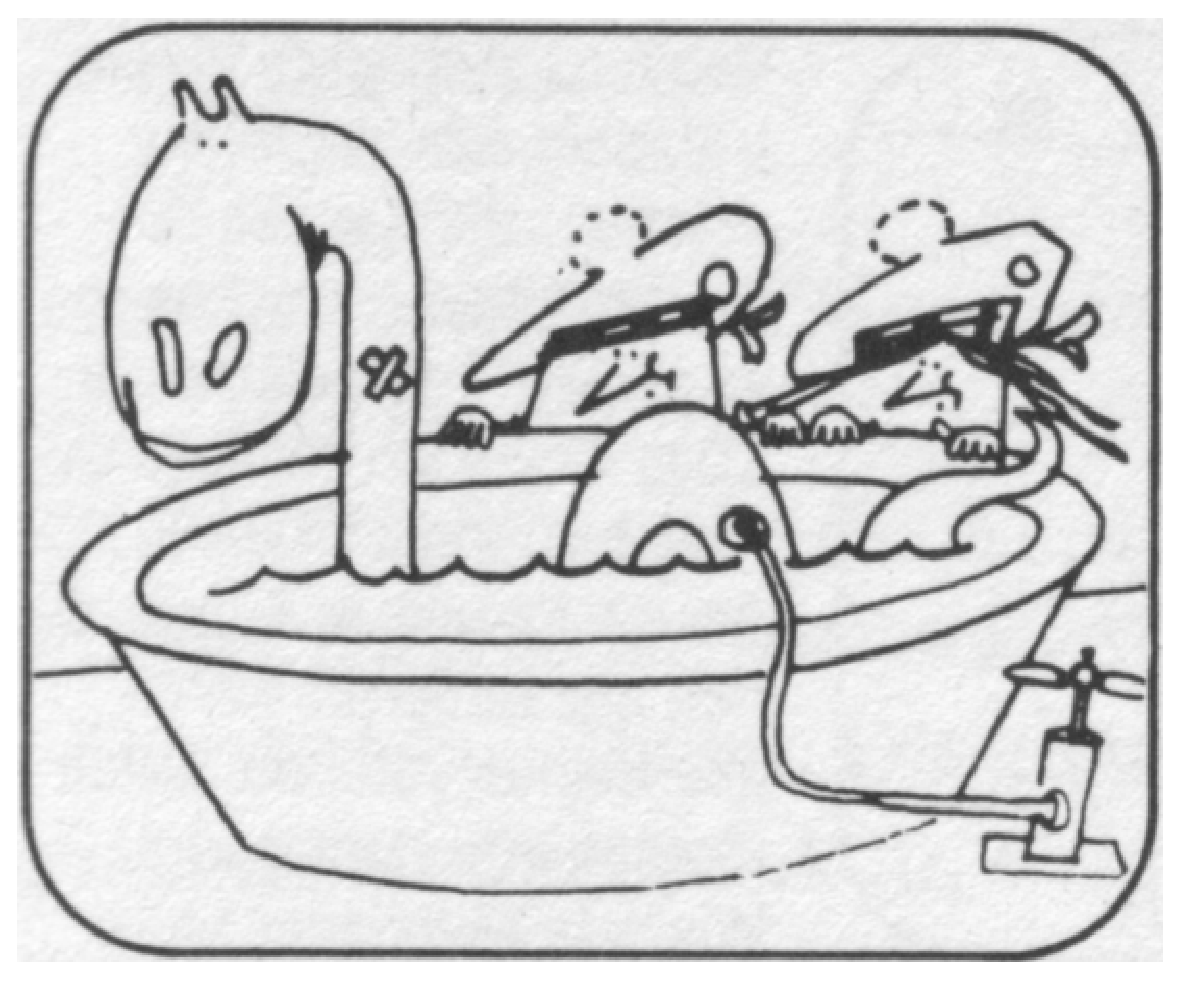
\includegraphics[width=0.618\textwidth]{pictures/lochness1.eps}}
\title{Gleichungen}
\subtitle{Wie gross ist Nessy?}
\author{}
\date{}
%\lowertitleback{
%\includegraphics[height=1.1cm]{/Users/jormawassmer/Pictures/logokoeniz.jpg}%
%\copyright Jorma Wassmer
%1. Auflage, Februar 2011
%}


\begin{document}
\maketitle
\tableofcontents
%\thispagestyle{empty}
\cleardoublepage
%\setcounter{page}{1}

\section{Aussageformen}
Wie man lineare Gleichungen l\"ost, wissen Sie schon. Aber was ist eine Gleichung eigentlich? Was tun wir beim L\"osen einer Gleichung genau und warum tun wir es? Wo tauchen pl\"otzlich ungeahnte Probleme auf? Letztlich geht es dabei auch darum, den Weg f\"ur andere Arten von Gleichungen zu ebnen, die wir noch nicht kennen.
\label{lingl}

\subsection{Das Monster von Loch Ness}
\label{lingl:lochness}

\medskip
\noindent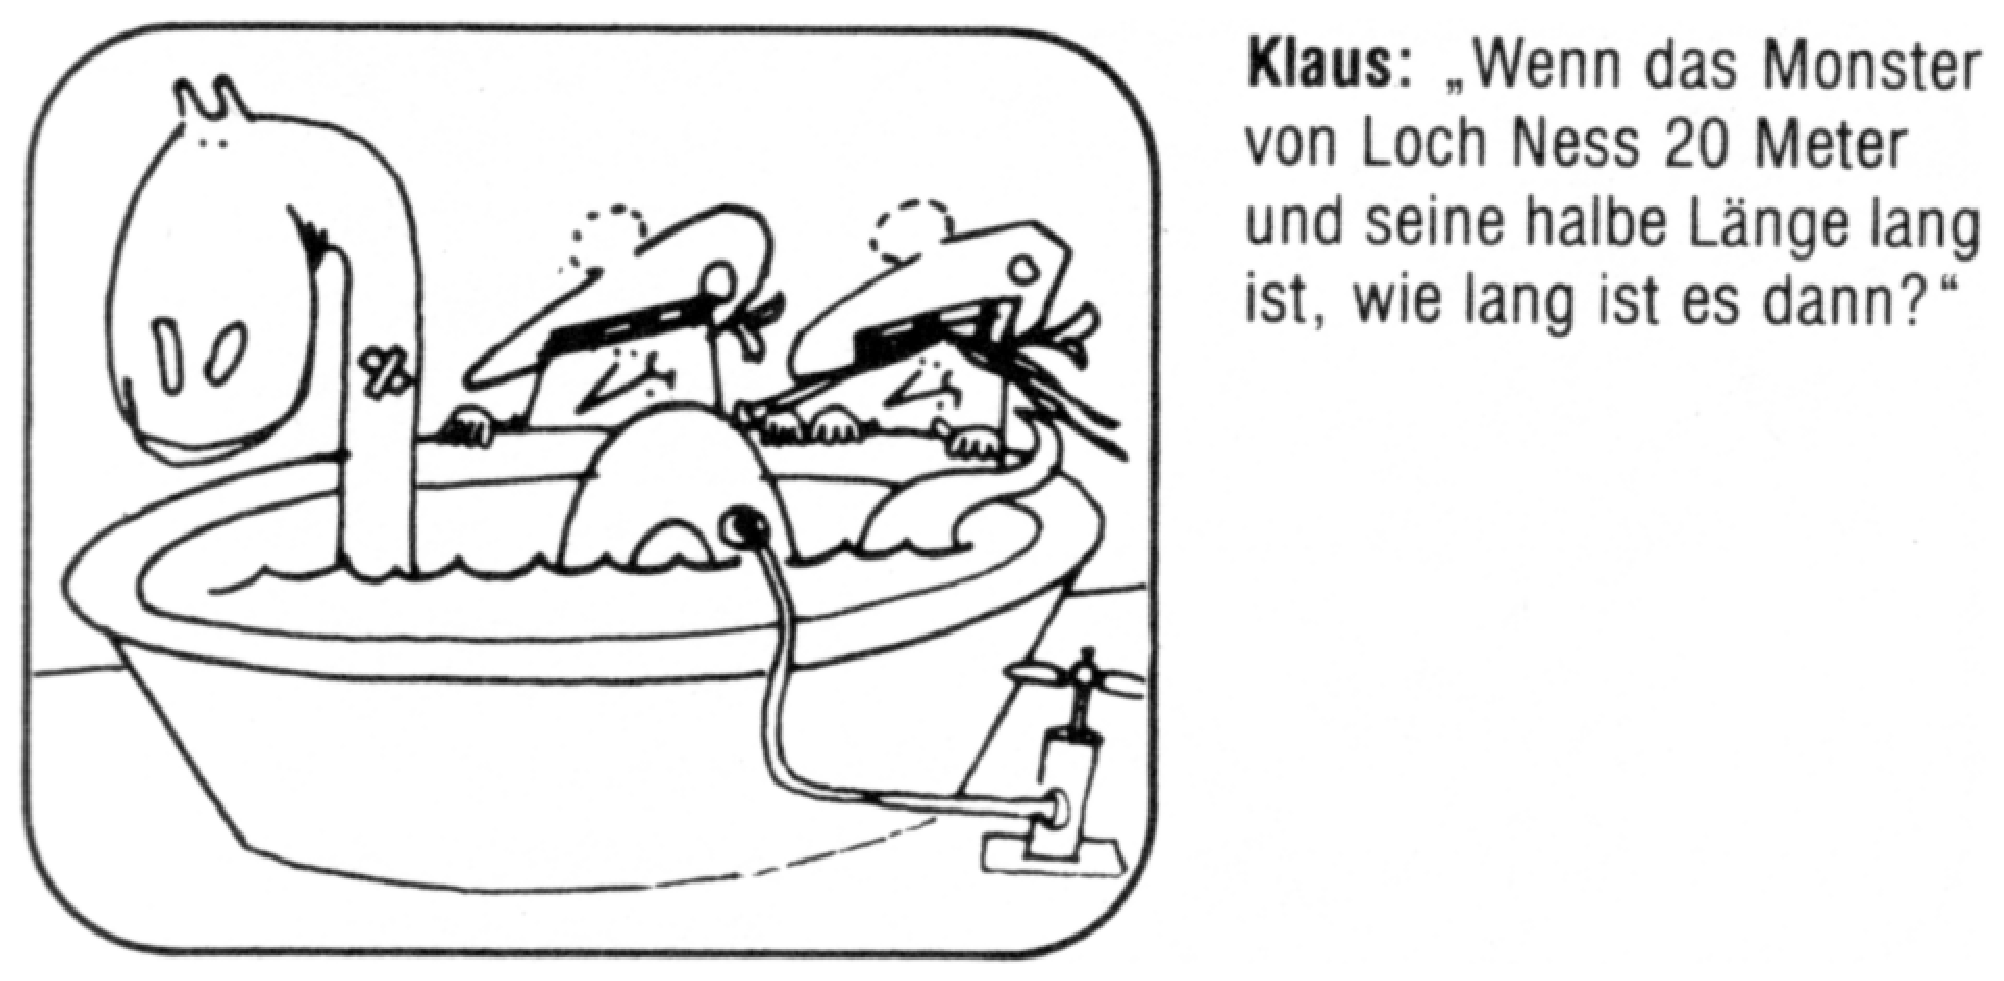
\includegraphics[width=\columnwidth,bb=14 14 960 469]{pictures/lochness1t.eps}

\medskip
\noindent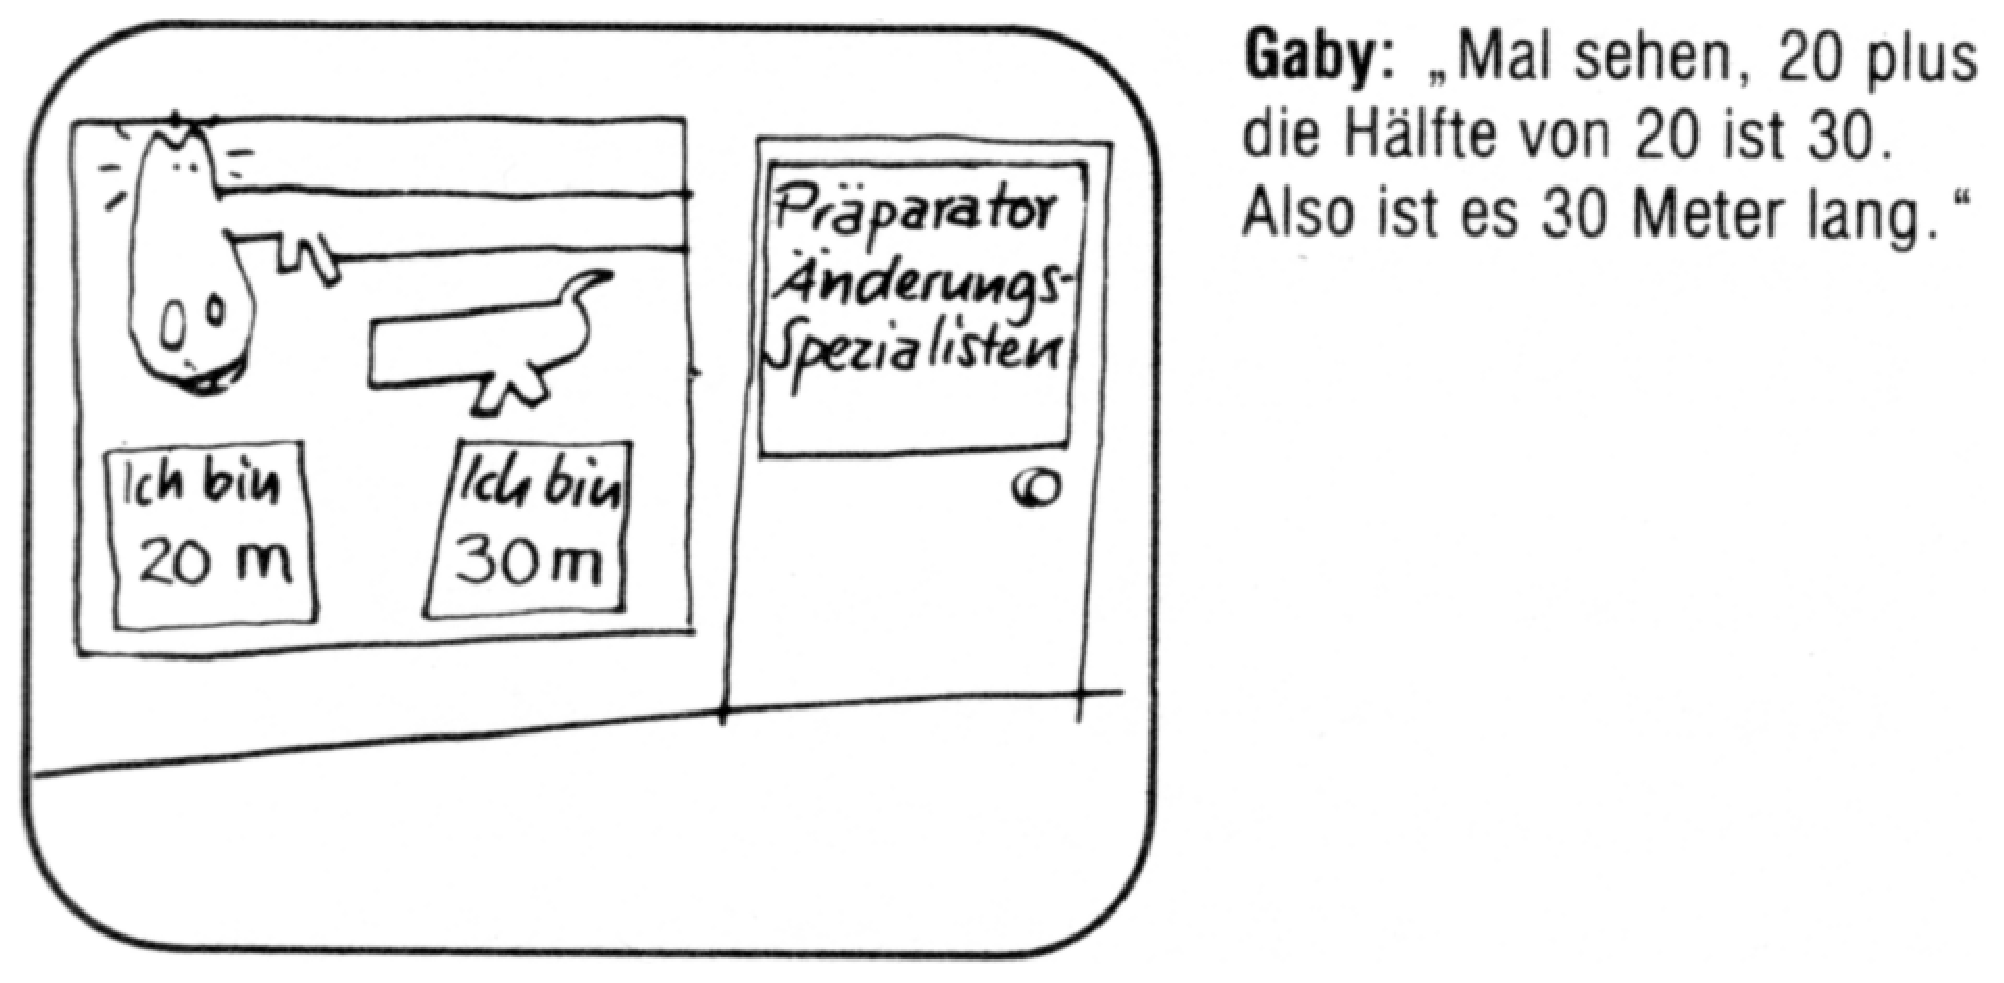
\includegraphics[width=\columnwidth,bb=14 14 960 470]{pictures/lochness2t.eps}

\medskip
\noindent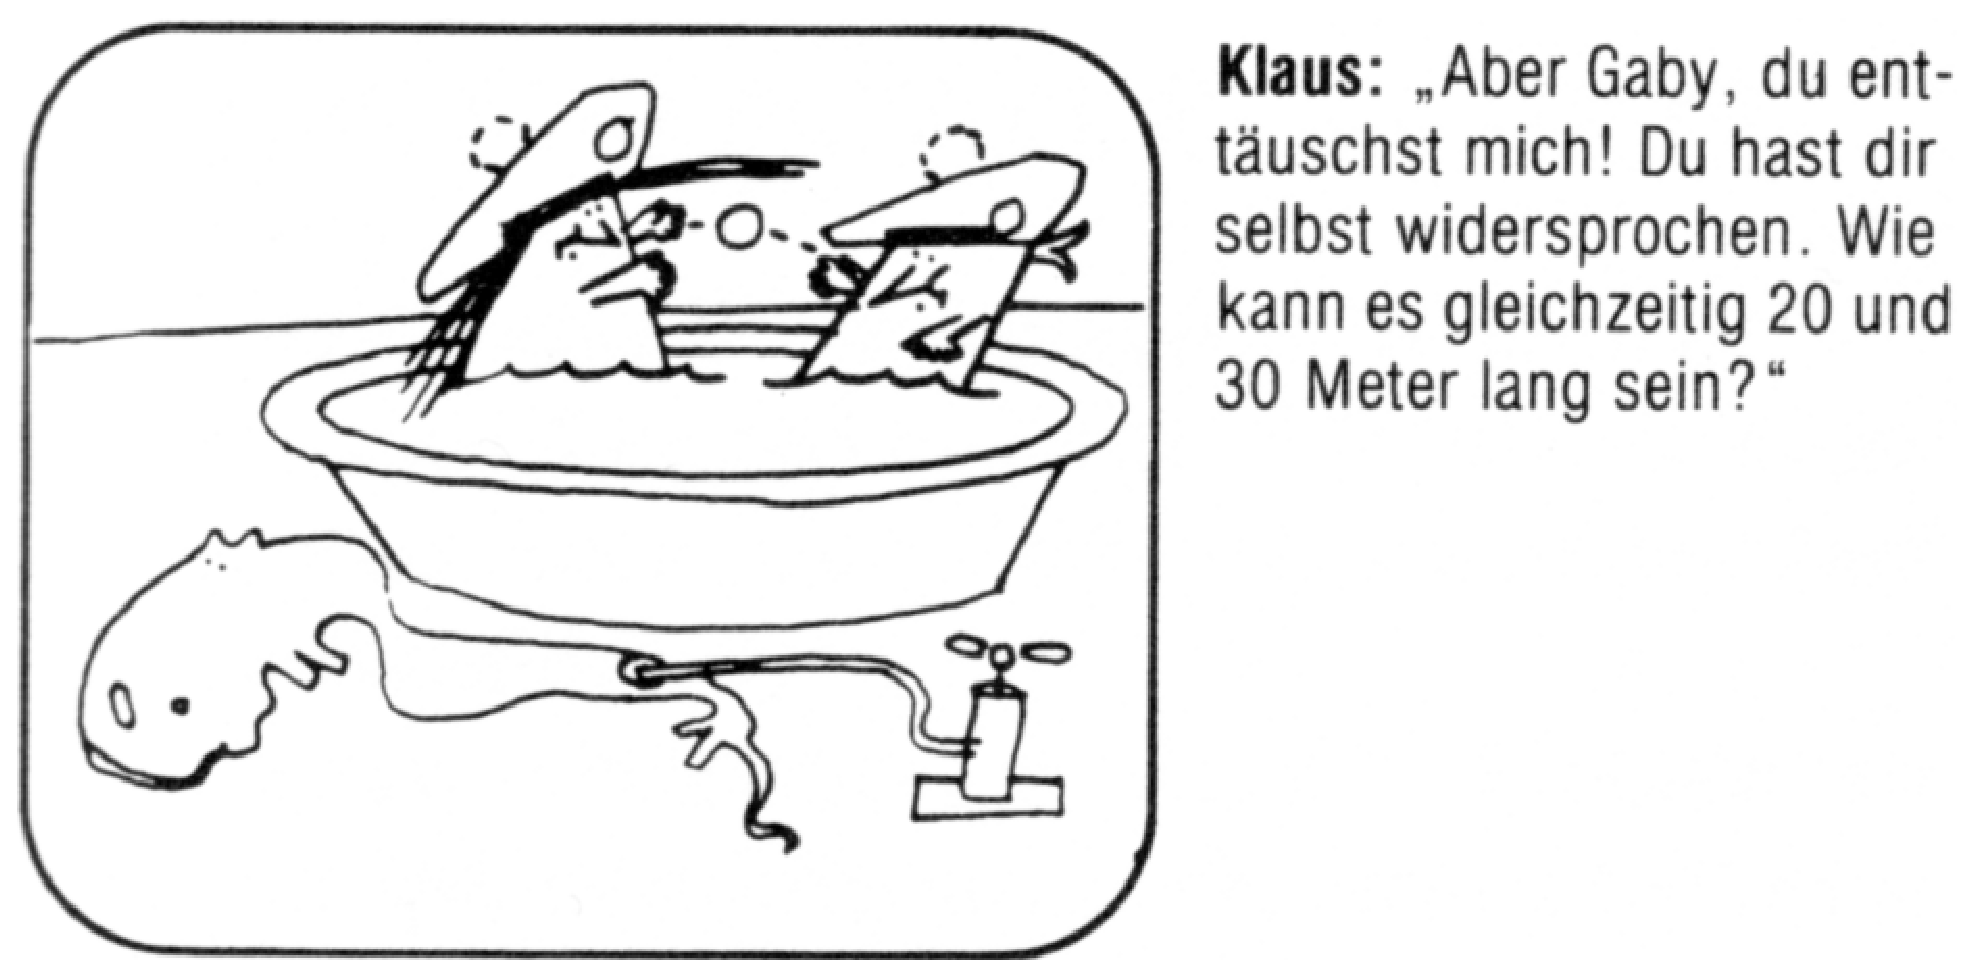
\includegraphics[width=\columnwidth,bb=14 14 946 468]{pictures/lochness3t.eps}

\enlargethispage{1ex}

\medskip
\noindent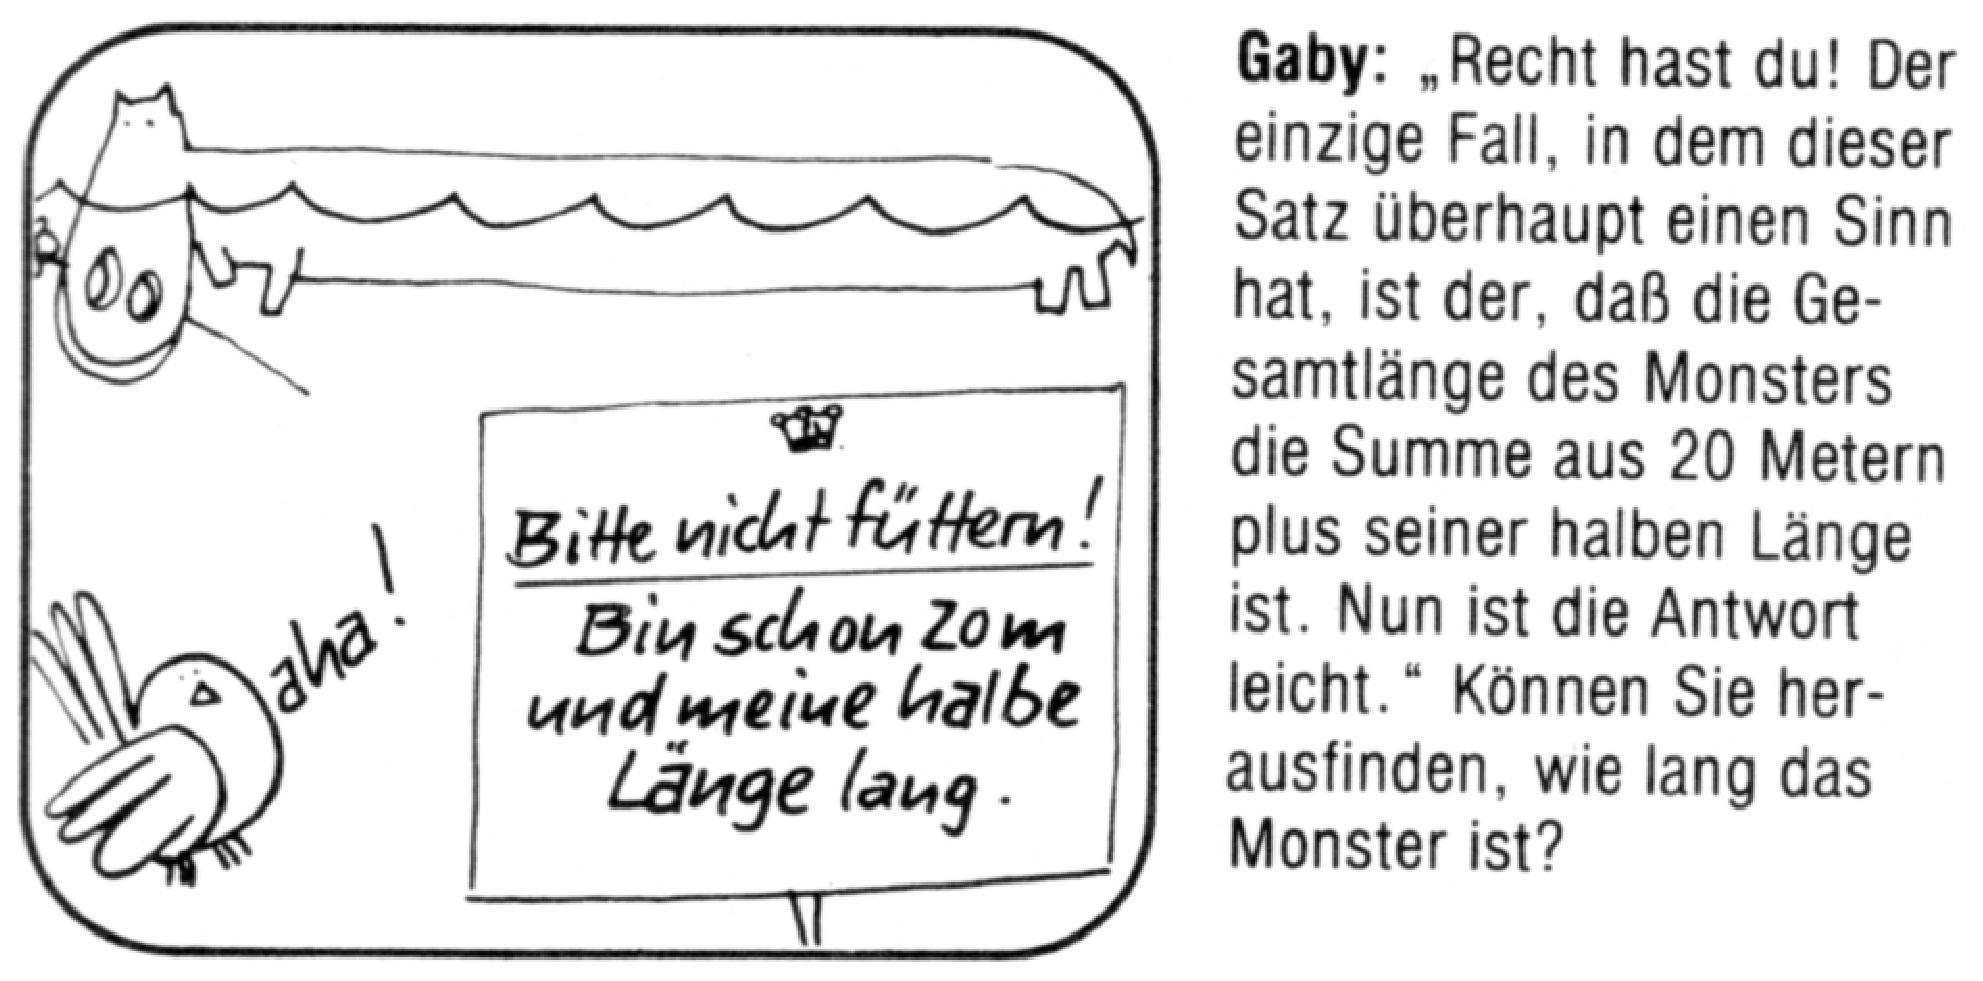
\includegraphics[width=\columnwidth,bb=14 14 950 469]{pictures/lochness4t.eps}

\label{lingl:ohnegl}

Wenn die Gesamtl\"ange des Monsters $\unit[20]{m}$ und seine halbe L\"ange ist, m\"ussen die erw\"ahnten $\unit[20]{m}$ die andere halbe L\"ange sein. Wenn $\unit[20]{m}$ die halbe L\"ange sind, dann ist die ganze $\unit[40]{m}$: Das Monster ist $\unit[40]{m}$ lang.

Auf diese Idee muss man allerdings zuerst kommen. Viele Probleme sind schwerer zu durchschauen. Dann hilft oft eine Gleichung weiter.

\label{lingl:gl}

Beim Aufstellen der Gleichung gehen wir wie folgt vor:

Was ist eigentlich gefragt? Die L\"ange des Monsters. Weil sie gefragt und somit unbekannt ist, bezeichnen wir sie mit einer Variablen (d.h. Unbekannten), z.B.:
\begin{center}
  $x$: L\"ange des Monsters
\end{center}
Dann \"ubersetzen wir das R\"atsel in eine Gleichung: Die L\"ange des Monsters ($x$) ist ($=$) $\unit[20]{m}$ und ($+$) seine halbe L\"ange ($\frac{x}{2}$) lang:
\begin{displaymath}
  x = \unit[20]{m} + \frac{x}{2}
\end{displaymath}
Wenn wir in dieser Gleichung $x=40\unit{m}$ einsetzen, stimmt sie tats\"achlich:
\begin{displaymath}
  \unit[40]{m} = \unit[20]{m}+\frac{\unit[40]{m}}{2}
\end{displaymath}
Gaby hat zun\"achst vermutet, das Monster k\"onnte $\unit[30]{m}$ lang sein, was sich aber als falsch erwiesen hat. Tats\"achlich stimmt die Gleichung nicht, wenn wir $x=\unit[30]{m}$ einsetzen:
\begin{displaymath}
  \unit[30]{m} \neq \unit[20]{m} + \frac{\unit[30] {m}}{2}
\end{displaymath}

\subsection{Was ist eine Gleichung eigentlich?}
\label{lingl:was}

Betrachten wir zun\"achst folgende ``Gleichungen'':
\begin{eqnarray*}
  \unit[40]{m} & = & \unit[20]{m}+\frac{\unit[40]{m}}{2} \\
  \unit[30]{m} & = & \unit[20]{m} + \frac{\unit[30]{m}}{2}
\end{eqnarray*}
Diese beiden ``Gleichungen'' sind Aussagen. Die erste ist wahr, die zweite falsch. Trotzdem sind beide Aussagen. 
\begin{cdef}[Aussage]{}
  Eine \emph{Aussage} ist ein Satz, von dem eindeutig entschieden werden kann, ob er wahr oder falsch ist.
\end{cdef}
Vergleichen wir das mit unserer Loch-Ness-Gleichung:
\begin{displaymath}
  x = \unit[20]{m} + \frac{x}{2}
\end{displaymath}
Hier kommt die Variable $x$ vor. Die Variable $x$ kann grunds\"atzlich f\"ur irgendeinen Wert stehen. D.h. f\"ur $x$ k\"onnen irgendwelche Werte eingesetzt werden. Wenn wir das tun, wird aus der Gleichung eine Aussage: Wenn wir $x=\unit[40]{m}$ einsetzen, wird sie zu einer wahren Aussage, f\"ur $x=\unit[30]{m}$ zu einer falschen.
\begin{cdef}[Aussageform]{}
  Eine Gleichung ist eine Aussage\emph{form}, die eine oder mehrere Variablen enth\"alt. Wenn wir f\"ur diese Variablen irgendwelche Zahlen einsetzen, wird die Gleichung zu einer (wahren oder falschen) Aussage.
\end{cdef}
F\"ur die meisten $x$ wird die Gleichung allerdings zu einer falschen Aussage. 
\begin{cdef}[Lösung]{}
  Ein $x$, f\"ur das die Gleichung zu einer wahren Aussage wird, nennen wir eine \emph{L\"osung} der Gleichung. 
\end{cdef}
Von den Beispielen her, die Ihnen bisher begegnet sind, sind Sie sich wohl gewohnt, dass eine Gleichung immer genau eine L\"osung hat. Es ist aber durchaus m\"oglich, dass eine Gleichung keine oder mehrere L\"osungen hat.
\begin{cdef}[Lösungsmenge]{}
  Die Menge aller L\"osungen einer Gleichung nennen wir die \emph{L\"osungsmenge} $L$.  
\end{cdef}
Die Loch-Ness-Gleichung hat nur eine L\"osung. Sie k\"onnen es probieren: Sie werden keine weitere L\"osung finden. Also ist die L\"osungsmenge:
\begin{displaymath}
  L=\{\unit[40]{m}\}
\end{displaymath}



\subsection{L\"osung durch Umformen der Gleichung}
\label{lingl:umformen}

Im Loch-Ness-Beispiel haben wir die L\"osung schon am Anfang gefunden. Diese L\"osung haben wir in die Gleichung eingesetzt und festgestellt, dass dadurch tats\"achlich eine wahre Aussage entsteht. Doch was tun wir, wenn wir die L\"osung der Gleichung nicht erraten k\"onnen? Sollen wir alle m\"oglichen Zahlen f\"ur $x$ einsetzen, bis wir die L\"osung(en) gefunden haben? Das kann ewig dauern. (Und das ist eindeutig zu lange.) Stattdessen k\"onnen wir die Gleichung umformen, wobei wir bei jedem Schritt auf beiden Seiten dieselbe Operation durchf\"uhren:

Gehen wir also nochmals von unserer Gleichung aus:
\begin{displaymath}
  x = \unit[20]{m} + \frac{x}{2}
\end{displaymath}
Zun\"achst subtrahieren wir beidseits $\frac{x}{2}$:
\begin{displaymath}
  \frac{x}{2} = \unit[20]{m}
\end{displaymath}
Dann multiplizieren wir beidseits mit 2:
\begin{displaymath}
  x = \unit[40]{m}
\end{displaymath}
Die L\"ange des Monsters ($x$) ist offensichtlich \unit[40]{m}. Tats\"achlich stimmt das mit der L\"osung \"uberein, die wir schon vorher gefunden haben.



\section{\"Aquivalenzumformungen}
\label{lingl:equiv}

Bei den Umformungen in Abschnitt \ref{lingl:umformen} haben wir am Schluss eine Gleichung erhalten, deren L\"osung wir leicht erraten k\"onnen. Wir wollen aber nicht die L\"osung der letzten Gleichung finden, sondern jene der ersten. Der Clou besteht nun darin, dass die L\"osungsmenge beim Umformen nicht ver\"andert wird.

Bei den Umformungen in Abschnitt \ref{lingl:umformen} war das der Fall. Tats\"achlich hat die Gleichung
\begin{displaymath}
  \frac{x}{2} = \unit[20]{m}  \; ,
\end{displaymath}
die wir durch Umformung aus der urspr\"unglichen erhalten haben, ebenfalls die L\"osungsmenge $L=\{\unit[40]{m}\}$. Weil bei den Umformungen die L\"osungsmenge nicht ver\"andert worden ist, k\"onnen wir von der L\"osung der letzten Gleichung auf jene der urspr\"unglichen Gleichung schliessen. Und das ist es ja, was wir letztlich suchen.

\begin{cdef}[Äquivalenz]{}
Wenn zwei Gleichungen dieselbe L\"osungsmenge haben, nennen wir sie \emph{\"aquivalent}.
\end{cdef}

Wir schreiben dann:
\begin{displaymath}
  x = \unit[20]{m} + \frac{x}{2} \quad\Leftrightarrow\quad \frac{x}{2} = \unit[20]{m}
\end{displaymath}
Der Doppelpfeil bedeutet, dass aus der ersten Gleichung die zweite folgt ($\Rightarrow$), und umgekehrt ($\Leftarrow$): Wenn f\"ur ein bestimmtes $x$ die erste Gleichung wahr (d.h. $x$ eine L\"osung) ist, gilt das auch f\"ur die zweite --- und umgekehrt. Dann sind beide L\"osungsmengen gleich.

Alle Gleichungen unserer Rechnung in Abschnitt \ref{lingl:umformen} sind \"aquivalent, d.h. sie haben dieselbe L\"osungsmenge, n\"amlich $L=\{\unit[40]{m}\}$. Die Umformungen haben also die L\"osungsmenge nicht ver\"andert.
\begin{cdef}[Äquivalenzumformung]{}
Eine Umformung, welche die L\"osungsmenge unver\"andert l\"asst, d.h. eine Gleichung in eine \"aquivalente \"uberf\"uhrt, nennen wir \emph{\"Aquivalenzumformung}.
\end{cdef}

Wenn wir auf beiden Seiten der Gleichung dasselbe tun, erhalten wir dann nicht immer eine \"aquivalente Gleichung? Nein. Dazu einige Beispiele und Gegenbeispiele:

\begin{itemize}
\item Addition mit derselben Zahl:
  \begin{displaymath}
    \begin{array}{rrclll}
      & x-5 & = & 2 \;\; & |\,+5 \quad & L = \{7\} \\
      \Leftrightarrow  & x & = & 7 & & L = \{7\}
    \end{array}
  \end{displaymath}
  
\item Division durch dieselbe Zahl ($\neq 0$):
  \begin{displaymath}
    \begin{array}{rrclll}
      & 2x & = & 8 \;\; & |\,:2 \quad & L = \{4\} \\
      \Leftrightarrow & x & = & 4 & & L = \{4\}
    \end{array}
  \end{displaymath}

\item Multiplikation mit derselben Zahl ($\neq 0$)
  \begin{displaymath}
    \begin{array}{rrclll}
      & -\frac{x}{3}-4 & = & 0 \, & |\,\cdot(-3) \, & L = \{-12\} \\
      \Leftrightarrow \!\!\! & x + 12 & = & 0 & &  L = \{-12\}
    \end{array}
  \end{displaymath}
  
\item Multiplikation mit 0:\footnote{$\nLeftrightarrow$ bedeutet `nicht \"aquivalent'.}
  \begin{displaymath}
    \begin{array}{rrclll}
      & 4x & = & 6 \;\; & |\,\cdot 0 \quad & L = \{\frac{3}{2}\} \\
      \nLeftrightarrow & 0 & = & 0 & & L = \mathbb{R}
    \end{array}
  \end{displaymath}
  In der zweiten Gleichung kommt $x$ gar nicht vor. Deshalb ist es egal, was $x$ ist. Die Gleichung ist f\"ur alle m\"oglichen $x$ wahr.

\item Quadrieren
  \begin{displaymath}
    \begin{array}{rrclll}
      & x & = & 2 \;\; & |\,(\;)^2 \quad & L = \{2\} \\
      \nLeftrightarrow & x^2 & = & 4 & & L = \{-2;2\}
    \end{array}
  \end{displaymath}
\end{itemize}

\begin{csatz}[Einige Äquivalenzumformungen]{}
Allgemein k\"onnen wir sagen: \"Aquivalenz"-umformungen sind (unter anderem):
\begin{itemize}
\item Beidseits dieselbe Zahl oder denselben Term addieren\footnote{Wenn $C<0$ ist, ergibt sich daraus eine Subtraktion.}:
  \begin{displaymath}
    A = B \quad\Leftrightarrow\quad A+C = B+C
  \end{displaymath}
\item Beidseits dieselbe Zahl $\neq 0$ oder denselben Term $\neq 0$ multiplizieren oder dividieren (d.h. $C \neq 0$):
  \begin{eqnarray*}
    A = B & \quad\Leftrightarrow\quad & A \cdot C = B \cdot C \\
    A = B & \quad\Leftrightarrow\quad & \frac{A}{C} = \frac{B}{C}
  \end{eqnarray*}
\end{itemize}
\end{csatz}




\section{Grundmenge}
\label{lingl:grundmenge}

Angenommen, das R\"atsel h\"atte so gelautet: \glqq Das Monster von Loch Ness ist 20\unit{m} und seine doppelte L\"ange lang.\grqq\ Dann h\"atten wir folgende Gleichung erhalten:
\begin{eqnarray*}
  x & = & \unit[20]{m}+2x \\
  -x & = & \unit[20]{m} \\
  x & = & \unit[-20]{m}
\end{eqnarray*}
Das Monster w\"are $-20\unit{m}$ lang. Aber es kann doch keine negative L\"ange haben! Von der Frage her sind nur positive L\"angen zugelassen.\footnote{Vielleicht w\"are eine negative L\"ange f\"ur ein Monster genau das Richtige. Wenn wir aber von einem real existierenden Monster ausgehen, dann muss es auch eine positive L\"ange haben. Ob die L\"ange Null auch zugelassen sein soll, dar\"uber kann man sich streiten. Die L\"ange Null w\"urde bedeuten, dass das Monster eben doch nicht existiert.} F\"ur $x$ kommen somit nur positive Zahlen in Frage. Mit negativen brauchen wir's gar nicht zu probieren. Wenn wir bei der Umformung dann doch zu einer negativen L\"osung kommen, dann wird sie disqualifiziert. Sie ist \emph{keine} L\"osung des Problems.

Es gibt also manchmal nur eine eingeschr\"ankte Menge von Zahlen, die f\"ur $x$ eingesetzt werden d\"urfen.\footnote{Das sieht man der Gleichung selbst nicht mehr an.} Diese Menge nennen wir \emph{Grundmenge}. 
\begin{quote}
  Die Grundmenge ist die Menge aller Zahlen, die f\"ur $x$ in Frage kommen.  
\end{quote}
Wenn $x$ z.B. eine Personenzahl ist, dann ist die Grundmenge noch st\"arker eingeschr\"ankt\footnote{sofern keine Brutalit\"aten zugelassen sind}: Die Grundmenge sind die nat\"urlichen Zahlen $\mathbb{N}$.

Als L\"osungen kommen nur Elemente aus der Grundmenge $G$ in Frage. Deshalb muss $L$ eine Teilmenge von $G$ sein:
\begin{displaymath}
  L \subset G
\end{displaymath}

\section{Lineare Gleichungen}
\label{lingl:lingl}

Wir wollen uns zun\"achst nur mit linearen Gleichungen besch\"aftigen. Linear sind Gleichungen, in welchen die gesuchte Variable (z.B. $x$) nur in der ersten Potenz vorkommt. Beispiele und Gegenbeispiele:

\begin{itemize}
\item lineare Gleichung:
  \begin{displaymath}
    3x - 5 = -7
  \end{displaymath}
\end{itemize}
Folgende Gleichungen sind nicht linear:
\begin{itemize}
\item quadratische Gleichung:
  \begin{displaymath}
    5x^2 + 2x - 8 = 0
  \end{displaymath}
  Das $x$ kommt im Quadrat vor.

\item Wurzelgleichung:
  \begin{displaymath}
    5\sqrt{9x+1} + 8x = 15
  \end{displaymath}
  Das $x$ kommt unter der Wurzel vor.

\item Exponentialgleichung:
  \begin{displaymath}
    5^{4x-3} = 16
  \end{displaymath}
  Das $x$ erscheint im Exponenten.
  
\end{itemize}


\subsection{L\"osungsstrategie f\"ur lineare Gleichungen}
\label{lingl:strategie}

Fassen wir zusammen: Die Gleichung wird (durch \"Aquivalenzumformungen) in eine \"aquivalente Gleichung umgeformt, deren L\"osungsmenge leicht zu erkennen ist. Die Ausgangsgleichung hat dann dieselbe L\"osungsmenge. Das Problem ist gel\"ost. Bei linearen Gleichungen gehen wir im Einzelnen so vor:
\begin{enumerate}
\item soweit n\"otig Klammern beseitigen (ausmultiplizieren) und vereinfachen
\item alle Summanden mit $x$ auf eine Seite bringen und alle Summanden ohne $x$ auf die andere
\item $x$ ausklammern
\item durch den mit $x$ multiplizierten Faktor dividieren
\item evtl. L\"osung durch Einsetzen in die Ausgangsgleichung testen (und Zugeh\"origkeit zur Grundmenge \"uberpr\"ufen)
\item evtl. L\"osungsmenge aufschreiben\footnote{Wenn die L\"osungsmenge klar ist, kann dieser Schritt weggelassen werden.}
\end{enumerate}

\"Ubrigens werden wir nicht jedesmal den \"Aquivalenzpfeil ($\Leftrightarrow$) schreiben, wenn zwei Gleichungen \"aquivalent sind, so wie wir's in den Beispielen von Abschnitt \ref{lingl:equiv} getan haben. Wenn wir eine Gleichung umformen, schreiben wir die neuen Gleichungen in der Regel einfach untereinander, in der Meinung, dass sie alle \"aquivalent zur Ausgangsgleichung sind.

\section{Algebra}
\label{lingl:algebra}

Das Aufl\"osen von Gleichungen (und Gleichungssystemen, wie wir es sp\"ater kennen lernen werden) wird als \emph{Algebra} bezeichnet. Dieser Begriff stammt aus dem Titel des arabischen Buches Kital al-mukhtasar fi hisab \emph{al-dschebr} w'al-mukabalah von \textsc{Mohammed Ibn Musa Al Chwarismi} (ca. 780--846), was frei \"ubersetzt Zusammenfassendes Buch \"uber das richtige Anordnen sowie das Ausgleichen bedeutet. Darin geht es um das L\"osen von Gleichungen. In diesem Zusammenhang heisst \emph{al-dschebr} soviel wie an die richtige Stelle bringen, was sich auf Zahlen und Variablen bezieht. Das illustriert die Pionierrolle der Araber auf dem Gebiet der Algebra.

In der modernen Mathematik wird der Begriff Algebra allerdings in einem viel umfassenderen Sinn verwendet. In der modernen Algebra wird nicht nur mit Zahlen (und Variablen, die daf\"ur stehen), sondern auch mit Mengen von anderen mathematischen Objekten operiert.


\section*{Übungen}

\begin{enumerate}
\item \label{aufg:lingl:lingl} Welche Gleichungen sind linear?

\begin{minipage}{0.5\textwidth}
  \begin{enumeratea}
  \item $\displaystyle x^2 + 5x = 10$
  \item $\displaystyle (x-1)5 = 37x + 1$ \label{aufg:lingl:lin1}
  \item $\displaystyle \sqrt{2}\,x = 11x - 8$ \label{aufg:lingl:lin2}
  \item $\displaystyle 2^x = 9x - 24$
  \end{enumeratea}
  \end{minipage}
  \begin{minipage}{0.5\textwidth}
  \begin{enumeratea}
  \setcounter{enumii}{4}
  \item $\displaystyle (x-3)(8-x)= 9+6x$
  \item $\displaystyle \sqrt{x-28} = 15$
  \item $\displaystyle x+21-x^5=0$
  \item $\displaystyle x=4$ \label{aufg:lingl:lin3}
  \end{enumeratea}
  \end{minipage}

\item Welche Gleichungspaare sind \"aquivalent und welche nicht?
  \begin{enumerate}
  \item \parbox{0.45\columnwidth}{$\displaystyle x-7=7$} \parbox{0.35\columnwidth}{$\displaystyle 3-x=-11$}
  \item \parbox{0.45\columnwidth}{$\displaystyle 4x=-8$} \parbox{0.35\columnwidth}{$\displaystyle 0=2+x$}
  \item \parbox{0.45\columnwidth}{$\displaystyle \frac{x}{3}=-2$} \parbox{0.35\columnwidth}{$\displaystyle -2x=3$}
  \item \parbox{0.45\columnwidth}{$\displaystyle 2x-x=x$} \parbox{0.35\columnwidth}{$\displaystyle 3=3$}
  \item \parbox{0.45\columnwidth}{$\displaystyle 2=1-x$} \parbox{0.35\columnwidth}{$\displaystyle x=2-1$}
  \item \parbox{0.45\columnwidth}{$\displaystyle 2x=\frac{2}{3}$} \parbox{0.35\columnwidth}{$\displaystyle x=3$}
  \item \parbox{0.45\columnwidth}{$\displaystyle 2x-2=2(x-1)$} \parbox{0.35\columnwidth}{$\displaystyle x=1$}
  \item \parbox{0.45\columnwidth}{$\displaystyle 3x-3x=0$} \parbox{0.35\columnwidth}{$\displaystyle x=0$}
  \item \parbox{0.45\columnwidth}{$\displaystyle -3x=0$} \parbox{0.35\columnwidth}{$\displaystyle 9x^2=0$}
  \end{enumerate}

\item Geben Sie die L\"osungsmengen der folgenden Gleichungen an, wenn die Grundmenge jeweils $\mathbb{N^*}$ (nat\"urliche Zahlen ohne Null), $\mathbb{Z}$ (ganze Zahlen) bzw. $\mathbb{R}$ (alle reellen Zahlen) ist.
  \begin{enumerate}
  \item $\displaystyle x+9=4$
  \item $\displaystyle 3-x=-5$
  \item $\displaystyle 2x-1=4$
  \end{enumerate}

\item Geben Sie die L\"osungsmengen der folgenden Gleichungen an. Die Grundmenge sei immer $\mathbb{R}$.

\begin{minipage}{0.5\textwidth}
  \begin{enumeratea}
  \item $\displaystyle \frac{3}{4}x + 15 = 51$
  \item $\displaystyle 5x-16 = 19-2x$
  \item $\displaystyle 0.8x+3-0.6x=1.2x-0.6-1.6x$
  \item $\displaystyle 10x-(6+4x)=18+5x$
  \item $\displaystyle 105-72x-53-69 \\ =55x+43x-23-170x+6$
  \item $\displaystyle 56x-43-52-19x \\ =7-72x-56x+165x-112$
  \item $\displaystyle 7(3x-6)+5(x-3)=11-4(17-x)$
  \item $\displaystyle 57-2(x+21)=23-2(x+4)$
  \item $\displaystyle 40-[3(2x-4)-2(2x-3)] \\ =60-2(x+5)-4$
  \item $\displaystyle \frac{18-2x}{9}-\frac{2}{3}=\frac{2}{9}x$
  \item $\displaystyle \frac{12+3x}{5}-3 = \frac{7-x}{3}-2$
  \end{enumeratea}
  \end{minipage}
  \begin{minipage}{0.5\textwidth}
  \begin{enumeratea}
  \setcounter{enumii}{11}
  \item $\displaystyle 5+\frac{1}{2}(11x-37)=3x+\frac{2}{5}(x+3)$
  \item $\displaystyle \frac{3(x-6)}{4}+15+\frac{2(x-3)}{3} \\[1ex] =25+\frac{x-1}{2}-\frac{x+13}{5}$
  \item $\displaystyle \frac{3x+5}{7}-\left(\frac{x+2}{3}-1\right) \\ =\frac{x+5}{3}-\frac{x-4}{2}$
  \item $\displaystyle (x+1)(4x-3) = 2(x+1)(2x+3)$
  \item $\displaystyle (x-5)(x-2)=(x-4)(x-3)$
  \item $\displaystyle (7x-5)(7-3x)-(6-5x)(3x-7) \\ =(3x-7)(7-2x)$
  \item $\displaystyle 3(x+1)(x+4)=(3x+6)(x+3)$
  \item $\displaystyle (x-3)(2x-5)-4(x-2) \\ =2(x-1)^2-12$
  \item $\displaystyle 2x^2-(x+3)(x-3)=(x+1)^2-2x+8$
  \item $\displaystyle (8-3x)^2+(5-4x)^2-6 \\ =(9-5x)^2+20x-4$
  \end{enumeratea}
  \end{minipage}
\end{enumerate}

\section*{L\"osungen}

\begin{enumerate}
\item a) nein, quadratisch, c) nein, Wurzel, d) nein, Exponentialgleichung, e) nein, quadratisch, f) neine Wurzelgleichung, g) nein, Gleichung vom Grad 5,
\item
  \begin{enumerate}
  \item $\displaystyle x-7=7 \Leftrightarrow 3-x=-11$ \\
    F\"ur beide Gleichungen ist $L=\{14\}$
  \item $\displaystyle 4x=-8 \Leftrightarrow 0=2+x$ \\
    F\"ur beide Gleichungen ist $L=\{-2\}$
  \item $\displaystyle \frac{x}{3}=-2 \nLeftrightarrow -2x=3$ \\
    1. Gleichung: $L_1=\{-6\}$; 2. Gleichung: $L_2=\{-\frac{3}{2}\}$. (Um von der ersten zur zweiten zu gelangen, wurde die 3 multipliziert; die $-2$ hingegen wurde rechts dividiert, links aber multipliziert.)
  \item $\displaystyle 2x-x=x \Leftrightarrow 3=3$ \\
    F\"ur beide Gleichungen ist $L=\mathbb{R}$. (F\"ur jedes $x$ sind beide Gleichungen erf\"ullt.)
  \item $\displaystyle 2=1-x \nLeftrightarrow x=2-1$ \\
    1. Gleichung: $L_1=\{-1\}$; 2. Gleichung: $L_2=\{1\}$ (Wenn in der 1. Gleichung die 1 subtrahiert wird, so steht rechts noch $-x$ und nicht $x$.)
  \item $\displaystyle 2x=\frac{2}{3} \nLeftrightarrow x=3$ \\
    1. Gleichung: $L_1=\{\frac{1}{3}\}$; 2. Gleichung: $L_2=\{3\}$. (Wenn in der ersten Gleichung die 2 dividiert wird, so steht rechts $\frac{1}{3}$ und nicht 3.)
  \item $\displaystyle 2x-2=2(x-1) \nLeftrightarrow x=1$ \\
    1. Gleichung: $L_1=\mathbb{R}$; 2. Gl.: $L_2=\{1\}$
  \item $\displaystyle 3x-3x=0 \nLeftrightarrow x=0$ \\
    1. Gleichung: $L_1=\mathbb{R}$; 2. Gl.: $L_2=\{0\}$
  \item $\displaystyle -3x=0 \Leftrightarrow 9x^2=0$
    F\"ur beide Gleichungen ist $L=\{0\}$. (Wenn wir die rechte Gleichung durch 9 dividieren, erhalten wir $x^2=0$. Zwar hat z.B. die Gleichung $x^2=1$ zwei L\"osungen ($L=\{-1;+1\}$), aber $x^2=0$ ist nur f\"ur 0 erf\"ullt, da $-0=+0$ ist.)
  \end{enumerate}

\item
  \begin{enumerate}
  \item $\displaystyle x+9=4$: \\
    $G=\mathbb{N^*}$: $L=\{\}$ \\
    $G=\mathbb{Z}$ und $G=\mathbb{R}$: $L=\{-5\}$
  \item $\displaystyle 3-x=-5$: \\
    f\"ur alle drei Grundmengen: $L=\{8\}$
  \item $\displaystyle 2x-1=4$: \\
    $G=\mathbb{N^*}$ und $G=\mathbb{Z}$: $L=\{\}$ \\
    $G=\mathbb{R}$: $L=\{\frac{5}{2}\}$
  \end{enumerate}

\item
  \begin{enumerate}
  \item $\displaystyle \frac{3}{4}x + 15 = 51$
    \begin{eqnarray*}
      \frac{3}{4}x & = & 36 \\
      x & = & \frac{4}{3} \cdot 36 = 48 \;\to\; L=\result{\{48\}}
    \end{eqnarray*}
  \item $\displaystyle 5x-16 = 19-2x$ 
    \begin{eqnarray*}
      5x & = & 35-2x \\
      7x & = & 35 \\
      x & = & 5 \;\to\; L=\result{\{5\}}
    \end{eqnarray*}
  \item $\displaystyle 0.8x+3-0.6x=1.2x-0.6-1.6x$ 
    \begin{eqnarray*}
      0.2x + 3 & = & -0.4x-0.6 \\
      0.6x + 3 & = & -0.6 \\
      0.6x & = & -3.6 \\
      x & = & -6 \;\to\; L= \result{\{-6\}}
    \end{eqnarray*}
  \item $\displaystyle 10x-(6+4x)=18+5x$
    \begin{eqnarray*}
      10x-6-4x & = & 18+5x \\
      6x - 6 & = & 18 + 5x \\
      x - 6 & = & 18 \\
      x & = & 24 \;\to\; L=\result{\{24\}}
    \end{eqnarray*}
  \item $\displaystyle 105-72x-53-69 \\ =55x+43x-23-170x+6$
    \begin{displaymath}
      -72x - 17 = -72x - 17
    \end{displaymath}
    Diese Gleichung ist f\"ur jedes $x\in\mathbb{R}$ erf\"ullt. Deshalb ist $L=\result{\mathbb{R}}$.
  \item $\displaystyle 56x-43-52-19x \\ =7-72x-56x+165x-112$
    \begin{eqnarray*}
      37x - 95 & = & 37x -105 \\
      37x & = & 37x - 10
    \end{eqnarray*}
    Diese Gleichung ist f\"ur kein $x$ erf\"ullt. Deshalb ist $L=\result{\{\}}$.
  \item $\displaystyle 7(3x-6)+5(x-3)=11-4(17-x)$
    \begin{eqnarray*}
      21x - 42 + 5x - 15 & = & 11 - 68 + 4x \\
      26x - 57 & = & 4x - 57 \\
      26x & = & 4x \\
      22x & = & 0 \\
      x & = & 0 \;\to\; L=\result{\{0\}}
    \end{eqnarray*}
    Beachten Sie: $L \neq \{\}\;$ Null ist auch eine Zahl, d.h. ein Element von Zahlenmengen\,\ldots!
  \item $\displaystyle 57-2(x+21)=23-2(x+4)$
    \begin{eqnarray*}
      57 - 2x - 42 & = & 23 - 2x - 8 \\
      15 - 2x & = & 15 - 2x \\
      L & = & \result{\mathbb{R}}
    \end{eqnarray*}
  \item $\displaystyle 40-[3(2x-4)-2(2x-3)] \\ =60-2(x+5)-4$
    \begin{eqnarray*}
      40 - [6x-12-4x+6] & = & 56 - 2x - 10 \\
      40 - [2x-6] & = & 46 - 2x \\
      40 - 2x + 6 & = & 46 - 2x \\
      46 - 2x & = & 46 - 2x \\
      L & = & \result{\mathbb{R}}
    \end{eqnarray*}
  \item $\displaystyle \frac{18-2x}{9}-\frac{2}{3}=\frac{2}{9}x$ \\
    Wir multiplizieren beide Seiten mit dem Hauptnenner, d.h. mit 9. So fallen alle Nenner weg:
    \begin{eqnarray*}
      18-2x - 2 \cdot 3 & = & 2x \\
      12 - 2x & = & 2x \\
      12 & = & 4x \\
      3 & = & x \;\to\; L=\result{\{3\}}
    \end{eqnarray*}
  \item $\displaystyle \frac{12+3x}{5}-3 = \frac{7-x}{3}-2$
    \begin{eqnarray*}
      \frac{12+3x}{5} & = & \frac{7-x}{3} + 1 \\
      3(12+3x) & = & 5(7-x) + 15 \quad |\;\cdot 3 \cdot 5 \\
      36 + 9x & = & 35 - 5x + 15 \\
      9x & = & 14 - 5x \\
      14x & = & 14 \\
      x & = & 1 \;\to\; L=\result{\{1\}}
    \end{eqnarray*}
  \item $\displaystyle 5+\frac{1}{2}(11x-37)=3x+\frac{2}{5}(x+3) \quad | \cdot 10$
    \begin{eqnarray*}
      50 + 5(11x-37) & = & 30x + 4(x+3) \\
      50 + 55x - 185 & = & 30x + 4x + 12 \\
      55x - 135 & = & 34x + 12 \\
      55x & = & 34x + 147 \\
      21x & = & 147 \\
      x & = & 7 \;\to\; L=\result{\{7\}}
    \end{eqnarray*}
  \item $\displaystyle \frac{3(x-6)}{4}+15+\frac{2(x-3)}{3} \\[1ex] =25+\frac{x-1}{2}-\frac{x+13}{5}$
    \begin{eqnarray*}
      \lefteqn{\frac{3(x-6)}{4}+\frac{2(x-3)}{3}} \hspace{1.5cm} \\
      & = & 10+\frac{x-1}{2}-\frac{x+13}{5} \quad |\;\cdot 60 \\
      \lefteqn{45(x-6) + 40(x-3)} \hspace{1.5cm} \\ 
      & = & 600 + 30(x-1) - 12(x+13) \\
      \lefteqn{45x-270+40x-120} \hspace{1.5cm} \\
      & = & 600+30x-30-12x-156 \\
      85x-390 & = & 414 + 18x \\
      67x & = & 804 \\
      x & = & 12 \;\to\; L=\result{\{12\}}
    \end{eqnarray*}
  \item $\displaystyle \frac{3x+5}{7}-\left(\frac{x+2}{3}-1\right) \\ =\frac{x+5}{3}-\frac{x-4}{2}$
    \begin{displaymath}
      \frac{3x+5}{7}-\frac{x+2}{3}+1 = \frac{x+5}{3}-\frac{x-4}{2}
    \end{displaymath}
    \begin{displaymath}
      \frac{3x+5}{7} + 1 = \frac{x+5+x+2)}{3} - \frac{x-4}{2} \quad |\;\cdot 42
    \end{displaymath}
    \begin{eqnarray*}
       6(3x+5) + 42 & = & 14(2x+7) - 21(x-4) \\
       18x + 30 + 42 & = & 28x+98 - 21x+84 \\
       18x + 72 & = & 7x + 182 \\
       11x & = & 110 \\
       x & = & 10 \;\to\; L=\result{\{10\}}
    \end{eqnarray*}
  \item $\displaystyle (x+1)(4x-3) = 2(x+1)(2x+3)$
    Wenn $x=-1$ ist, dann sind beide Seiten Null und somit ist die Gleichung erf\"ullt. $x=-1$ ist also eine L\"osung der Gleichung. 

Wenn $x\neq -1$ ist, dann k\"onnen wir beidseits durch $(x+1)$ dividieren. (Wenn $x=-1$ ist, d\"urfen wir das nicht, weil wir dann durch 0 dividieren w\"urden.)
    \begin{eqnarray*}
      4x-3 & = & 2(2x+3) \\
      4x-3 & = & 4x+6 \\
      4x & = & 4x + 9
    \end{eqnarray*}
    Diese Gleichung ist f\"ur kein $x$ erf\"ullt. Somit ist $x=-1$ die einzige L\"osung: $L=\result{\{-1\}}$. (Zu diesem Ergebnis kommen wir letztlich auch, wenn wir die Ausgangsgleichung ausmultiplizieren und nach $x$ aufl\"osen\,\ldots)
  \item $\displaystyle (x-5)(x-2)=(x-4)(x-3)$
    \begin{eqnarray*}
      x^2 -2x -5x +10 & = & x^2-3x-4x+12 \\
      -7x + 10 & = & -7x + 12 \\
      -7x & = & -7x + 2 \\
      L & = & \result{\{\}}
    \end{eqnarray*}
  \item $\displaystyle (7x-5)(7-3x)-(6-5x)(3x-7) \\ =(3x-7)(7-2x)$

    Der Faktor $(7-3x)$ kommt in jedem Summanden vor, wenn wir mit Hilfe des Vorzeichentricks einen Teil der Differenzen umkehren:
    \begin{eqnarray*}
       (7x-5)(7-3x)+(6-5x)(7-3x) \\ =(7-3x)(2x-7)
    \end{eqnarray*}
    Wenn $7-3x=0$ ist, d.h. f\"ur $x=\frac{7}{3}$, sind alle Summanden Null und die Gleichung somit erf\"ullt. $x=\frac{7}{3}$ ist also eine L\"osung. Wenn $7-3x\neq 0$ ist, dann k\"onnen wir beide Seiten durch diesen Faktor dividieren:
    \begin{eqnarray*}
      7x-5 + 6-5x & = & 2x-7 \\
      2x + 1 & = & 2x - 7 \\
      2x & = & 2x - 8
    \end{eqnarray*}
    Diese Gleichung ist f\"ur kein $x$ erf\"ullt. Somit ist $x=\frac{7}{3}$ die einzige L\"osung: $L=\result{\{\frac{7}{3}\}}$.
  \item $\displaystyle 3(x+1)(x+4)=(3x+6)(x+3)$
    \begin{eqnarray*}
      3(x^2+4x+x+4) & = & 3x^2+9x+6x+18 \\
      3x^2+15x+12 & = & 3x^2 +15x+18 \\
      15x & = & 15x + 6 \\
      L & = & \result{\{\}}
    \end{eqnarray*}
  \item $\displaystyle (x-3)(2x-5)-4(x-2) \\ =2(x-1)^2-12$
    \begin{eqnarray*}
      \lefteqn{2x^2-5x-6x+15-4x+8} \hspace{2cm}\\
      & = & 2x^2-4x+2-12 \\
      -15x+23 & = & -4x-10 \\
      33 & = & 11x \\
      3 & = & x \;\to\; L=\result{\{3\}}
    \end{eqnarray*}
  \item $\displaystyle 2x^2-(x+3)(x-3)=(x+1)^2-2x+8$
    \begin{eqnarray*}
      2x^2-x^2+9 & = & x^2+2x+1 - 2x +8 \\
      x^2 + 9 & = & x^2 + 9 \\
      L & = & \result{\mathbb{R}}
    \end{eqnarray*}
  \item $\displaystyle (8-3x)^2+(5-4x)^2-6 \\ =(9-5x)^2+20x-4$
    \begin{eqnarray*}
      64-48x+9x^2 + 25-40x+16x^2 - 6 \\
      = 81-90x+25x^2+20x-4
    \end{eqnarray*}
    \begin{eqnarray*}
      25x^2 - 88x +83 & = & 25x^2 - 70x + 77 \\
      6 & = & 18x \\
      \frac{1}{3} & = & x \;\to\; L=\result{\{\frac{1}{3}\}}
    \end{eqnarray*}
  \end{enumerate}

\end{enumerate}

\label{lingltext}

\section{Lineare Gleichungen mit 2 Unbekannten}

\medskip
	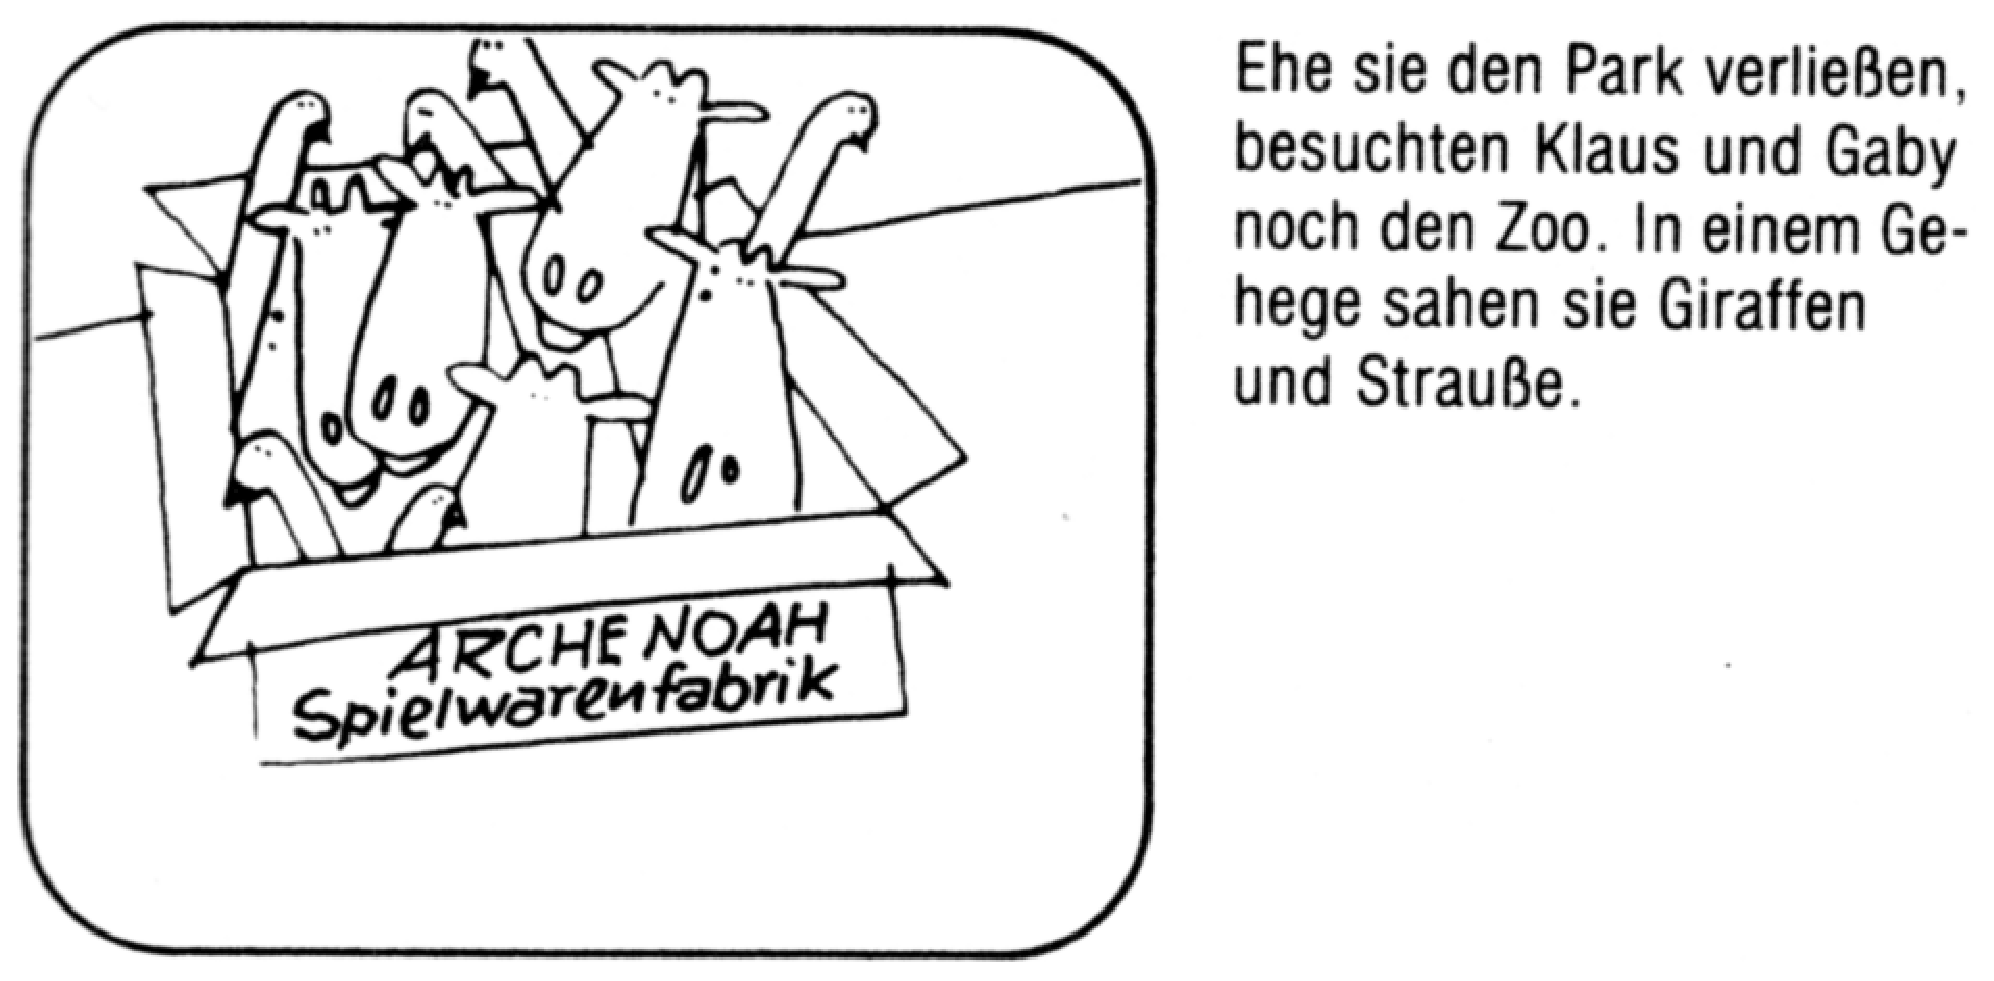
\includegraphics[width=0.9\columnwidth,bb=14 14 954 470]{pictures/augenbeine1t.eps}

\medskip
	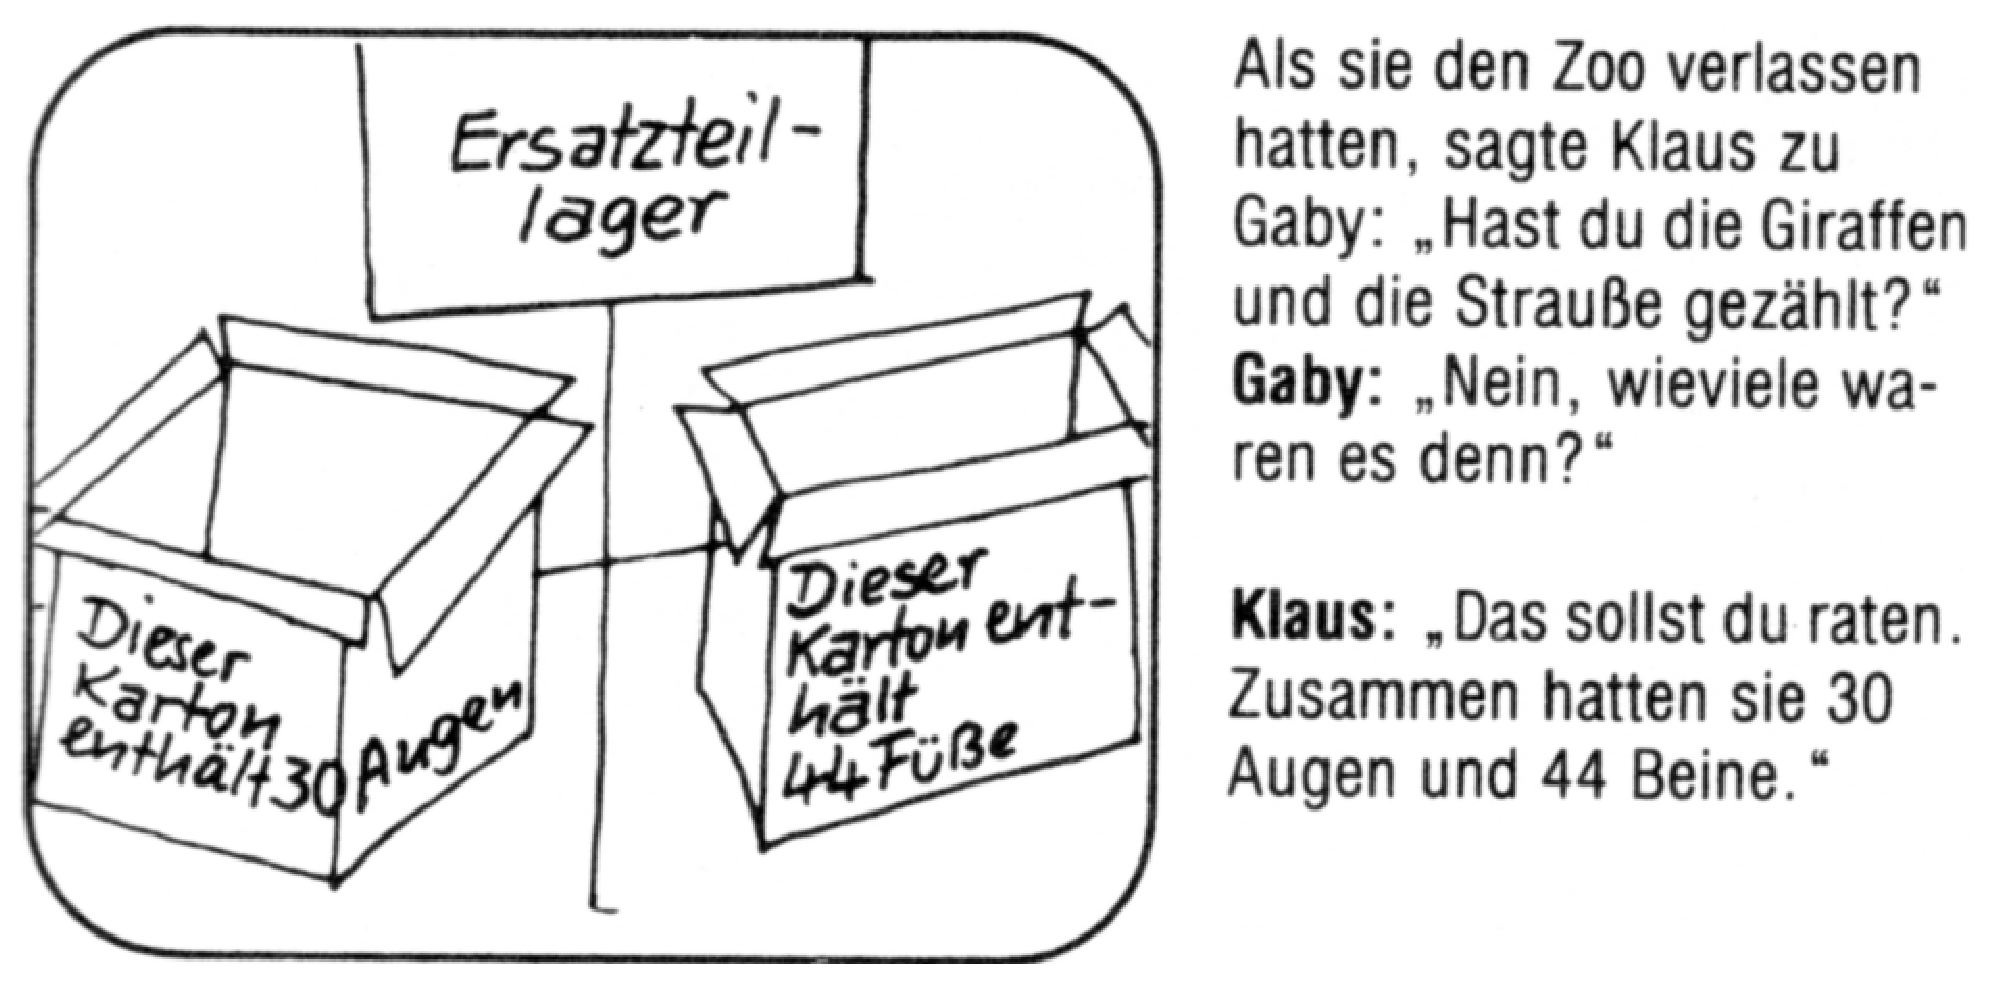
\includegraphics[width=0.9\columnwidth,bb=14 14 954 470]{pictures/augenbeine2t.eps}

\medskip
	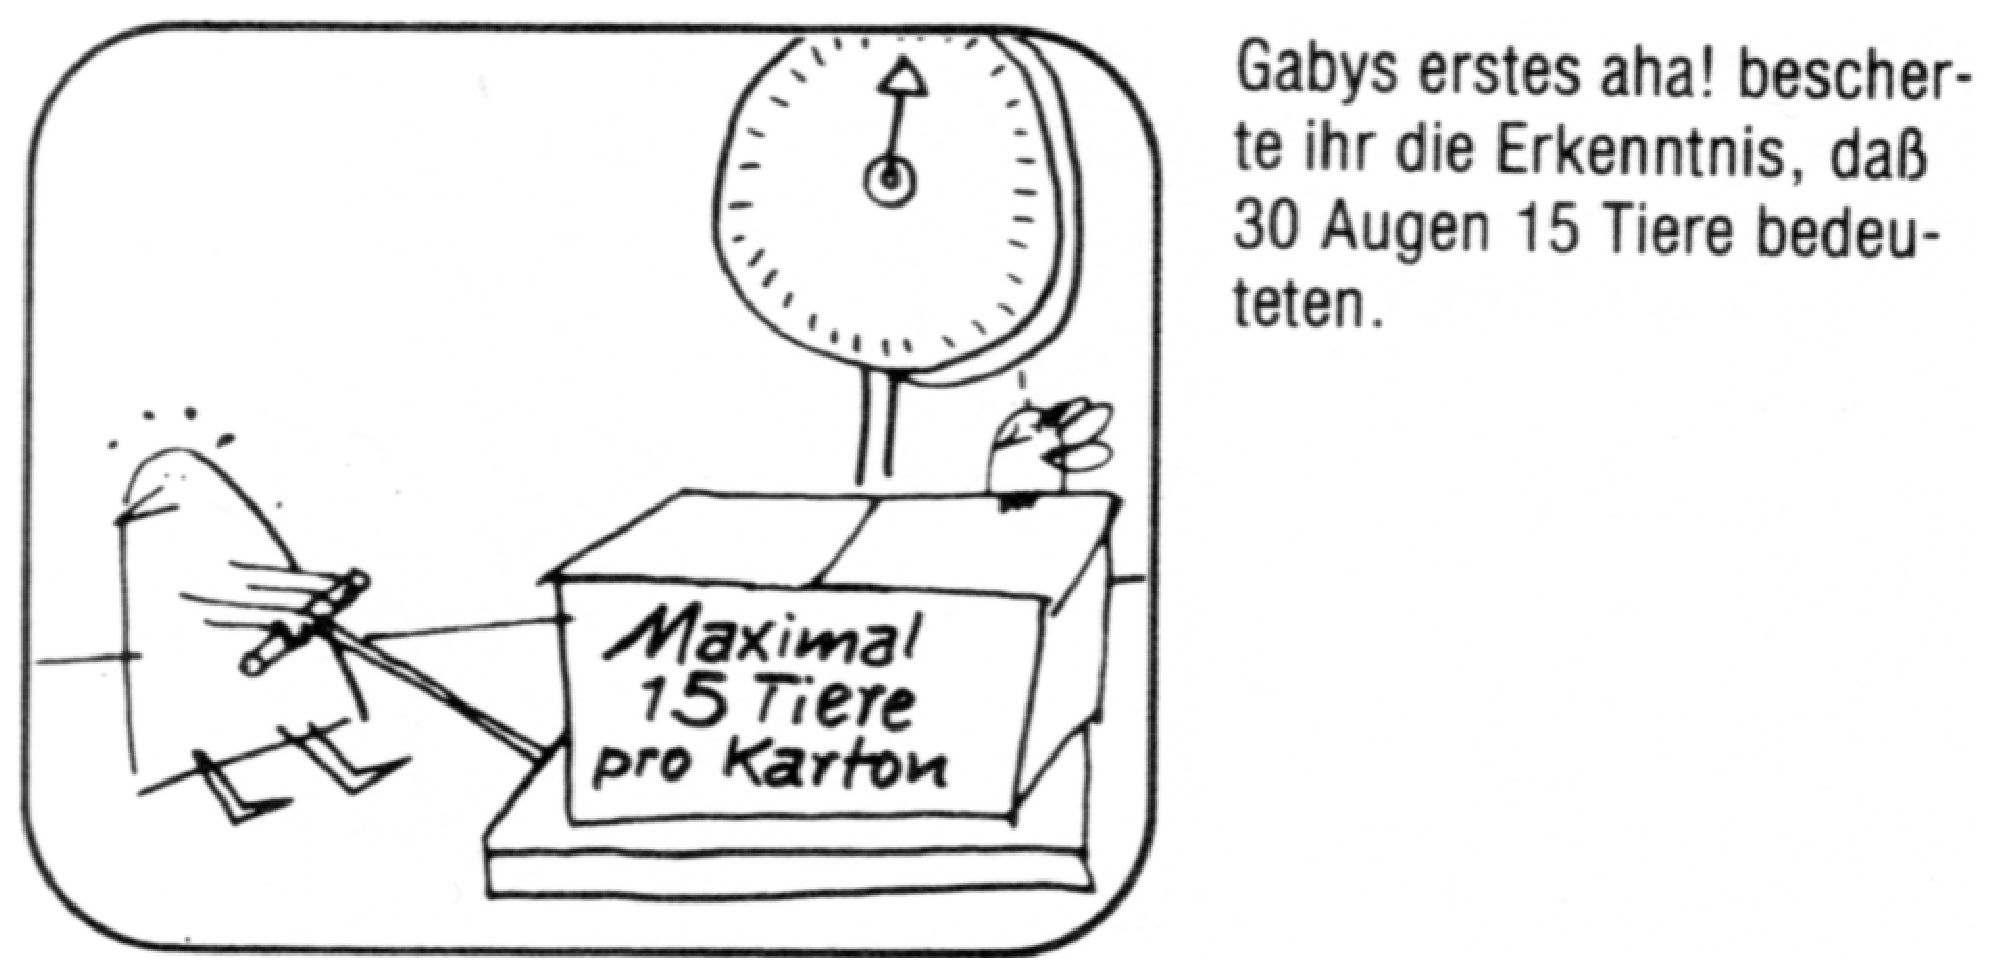
\includegraphics[width=0.9\columnwidth,bb=14 14 956 467]{pictures/augenbeine3t.eps}

\medskip
	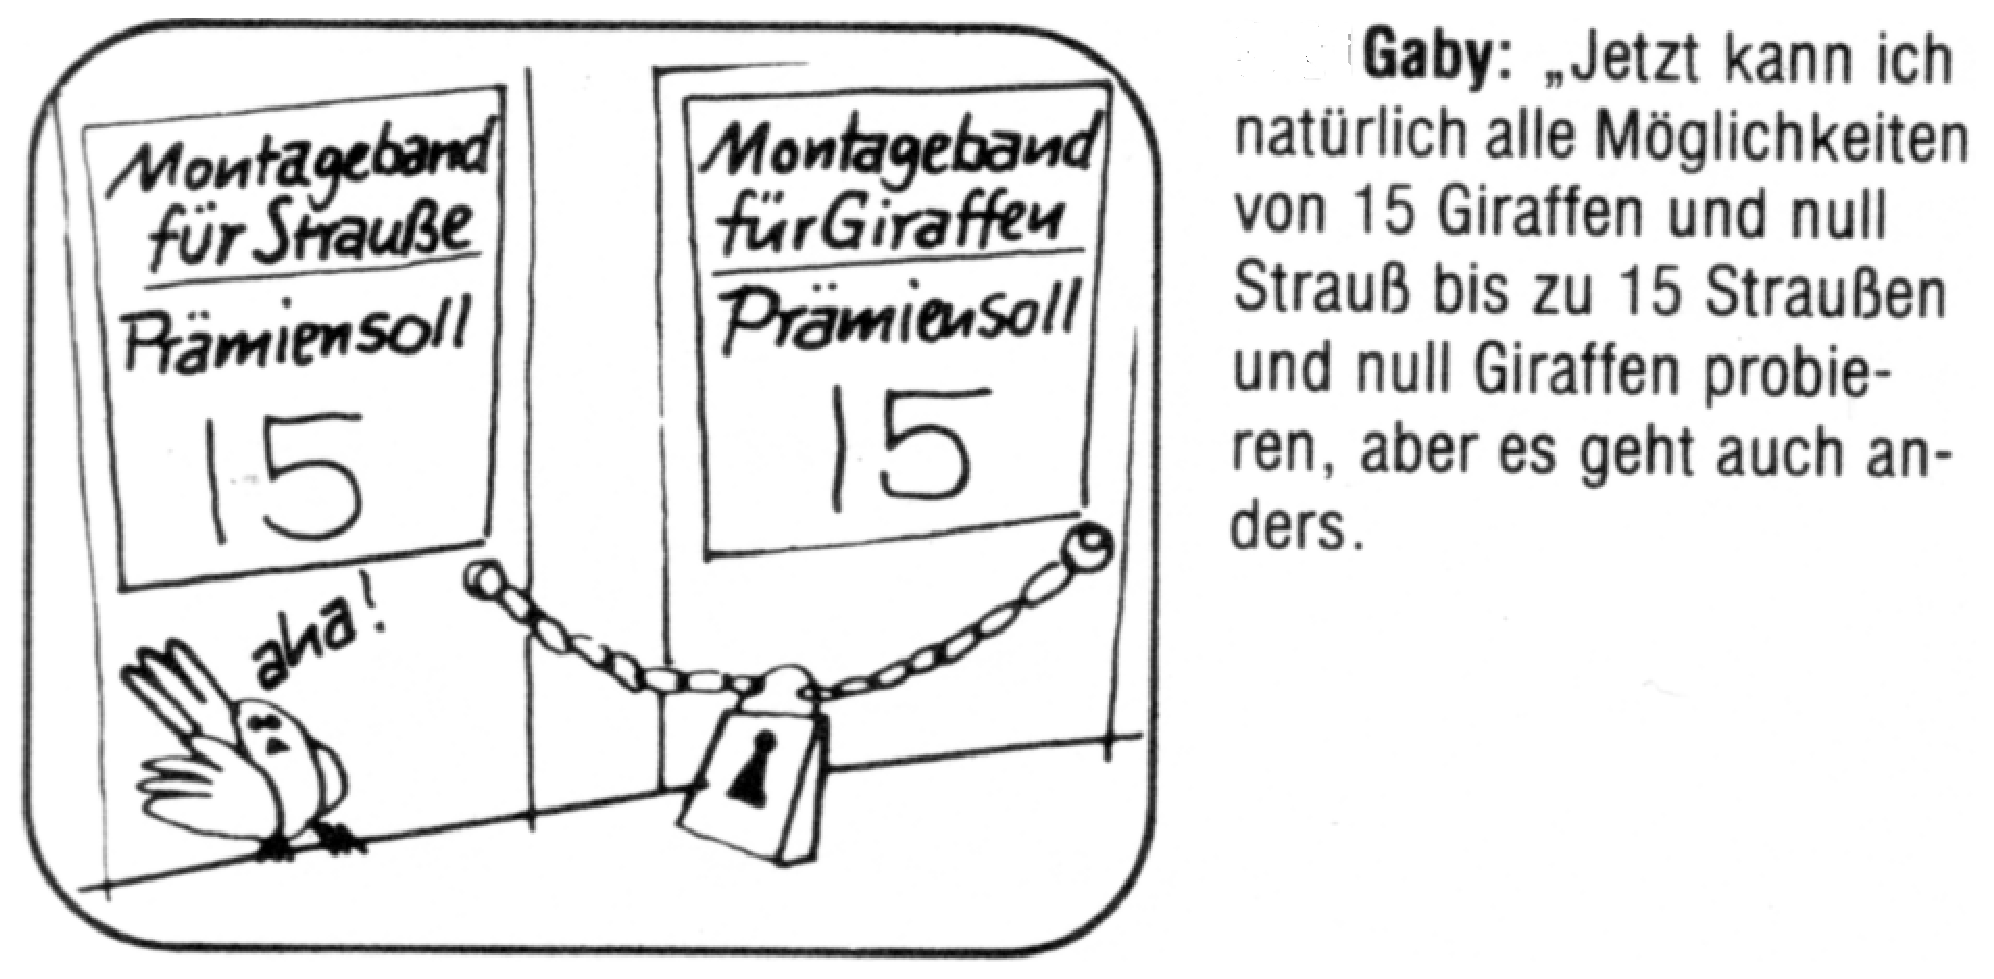
\includegraphics[width=0.9\columnwidth,bb=14 14 955 468]{pictures/augenbeine4t.eps}

\medskip

Klaus fragt, wieviele Strausse und wieviele Giraffen es hat. Dazu macht er zwei Aussagen:
\begin{itemize}
\item Es sind insgesamt 15 Tiere.
\item Zusammen haben sie 44 Beine.
\end{itemize}
Diese beiden Aussagen k\"onnen wir in die algebraische Sprache \"ubersetzen. Dazu geben wir den gefragten Zahlen je einen Namen:
\begin{itemize}
  \item $x$: Anzahl Strausse
  \item $y$: Anzahl Giraffen
\end{itemize}
Insgesamt sind es 15 Tiere, also gilt:
\begin{displaymath}
  x+y = 15
\end{displaymath}
Zusammen haben sie 44 Beine. Jeder Strauss hat zwei Beine; also haben alle Strausse zusammen $2x$ Beine. Jede Giraffe hat vier Beine; also haben alle Giraffen zusammen $4y$ Beine. Alle Beine zusammen:
\begin{displaymath}
  2x+4y=44
\end{displaymath}
Wir haben nun zwei Gleichungen. Diese beiden Gleichungen sind aber nicht unabh\"angig voneinander. D.h. es reicht nicht, wenn wir ein Paar $(x_1|y_1)$ finden, f\"ur das die erste Gleichung erf\"ullt ist, und ein anderes Paar $(x_2|y_2)$, f\"ur das die zweite Gleichung stimmt. Das R\"atsel verlangt, dass f\"ur \emph{eine} bestimmte Straussenzahl $x$ und \emph{eine} bestimmte Giraffenzahl $y$ \emph{beide} Bedingungen erf\"ullt sind. Beide Gleichungen geh\"oren zusammen und m\"ussen f\"ur dasselbe Paar $(x|y)$ erf\"ullt sein. Wir sprechen daher von einem \emph{Gleichungssystem mit zwei Gleichungen und zwei Variablen}. Um deutlich zu machen, dass es sich um ein Gleichungssystem handelt, und nicht um zwei unabh\"angige Gleichungen, schreiben wir:
\begin{system}
  x+y & = & 15 \\
  2x+4y & = & 44
\end{system}Manchmal lassen wir die beiden Striche links und rechts weg, wenn wir annehmen, es sei klar, dass es sich um ein Gleichungssystem handelt.

\label{linglsyst:probieren}

Doch wie finden wir das Paar $x$ und $y$, f\"ur das beide Gleichungen erf\"ullt sind? Gaby schl\"agt vor, alle M\"oglichkeiten durchzuprobieren. Tun wir das! Wir probieren alle M\"oglichkeiten von null Strauss bis zu 15 Straussen, d.h. von $x=0$ bis $x=15$. Dazu machen wir uns die \ref{tab:linglsyst:erste}.

\begin{table}[b!]
  \centering
  \begin{tabular}{|c|c|c|c|}
    \hline
    Strausse & Giraffen & Beine & $2x+4y$ \\
    $x$ & $y=15-x$ & $2x+4y$ & $=44$ \\ \hline\hline
    0 & 15 & 60 & $f$ \\ \hline
    1 & 14 & 58 & $f$ \\ \hline
    2 & 13 & 56 & $f$ \\ \hline
    3 & 12 & 54 & $f$ \\ \hline
    4 & 11 & 52 & $f$ \\ \hline
    5 & 10 & 50 & $f$ \\ \hline
    6 & 9 & 48 & $f$ \\ \hline
    7 & 8 & 46 & $f$ \\ \hline
    8 & 7 & 44 & $\surd$ \\ \hline
    9 & 6 & 42 & $f$ \\ \hline
    10 & 5 & 40 & $f$ \\ \hline
    11 & 4 & 38 & $f$ \\ \hline
    12 & 3 & 36 & $f$ \\ \hline
    13 & 2 & 34 & $f$ \\ \hline
    14 & 1 & 32 & $f$ \\ \hline
    15 & 0 & 30 & $f$ \\ \hline
  \end{tabular}
  \caption{Wir probieren alle M\"oglichkeiten von null Strauss und 15 Giraffen bis zu 15 Straussen und null Giraffen durch. Das $y$ w\"ahlen wir dabei immer so, dass die erste Gleichung (die wir nach $y$ aufgel\"ost haben) erf\"ullt ist. Wir berechnen dann die Anzahl Beine, die sich f\"ur das Paar $(x|y)$ ergeben und pr\"ufen ob es 44 sind, d.h. ob die zweite Gleichung erf\"ullt ist. In der hintersten Spalte markieren wir dies mit $f$ f\"ur \begriff{falsch} bzw. $\surd$ f\"ur \begriff{richtig}.}
  \label{tab:linglsyst:erste}
\end{table}

Wir sehen, dass f\"ur $x=8$ und $y=7$ beide Gleichungen, d.h. beide Bedingungen erf\"ullt sind. Die Antwort lautet also: Es sind 8 Strausse und 7 Giraffen. Tats\"achlich: Das sind 15 Tiere und sie haben $8 \cdot 2 + 7 \cdot 4 = 44$ Beine.

\subsection{Gemeinsame L\"osung mit try and error suchen}
\label{linglsyst:heraussuchen}

In den ersten beiden Spalten von \ref{tab:linglsyst:erste} sind alle Paare $(x|y)$ aufgelistet, f\"ur welche die erste Gleichung ($x+y=15$) erf\"ullt ist. Das sind alle M\"oglichkeiten, f\"ur die es insgesamt 15 Tiere gibt. Alle diese Paare sind L\"osungen der Gleichung. Zusammen bilden sie somit die L\"osungsmenge der ersten Gleichung:
\begin{eqnarray*}
  L_1 & = & \{(0|15),(1|14),(2|13),(3|12),(4|11), \\
  & & (5|10),(6|9),(7|8),(8|7),(9|6),(10|5), \\ 
  & & (11|4),(12|3),(13|2),(14|1),(15|0)\}
\end{eqnarray*}
In den beiden anderen Kolonnen von \ref{tab:linglsyst:erste}) haben wir gepr\"uft, f\"ur welches Paar $(x|y)$ die zweite Gleichung erf\"ullt ist. Wir k\"onnten aber auch eine Tabelle aller Paare $(x|y)$ erstellen, f\"ur welche die zweite Gleichung erf\"ullt ist, f\"ur die es also 44 Beine gibt. Alle diese Paare w\"urden dann die L\"osungsmenge $L_2$ der zweiten Gleichung bilden. Dann k\"onnten wir schauen, ob ein Paar in beiden Tabellen bzw. L\"osungsmengen vorkommt. Dieses Paar w\"urde beide Gleichungen erf\"ullen und w\"are somit die L\"osung des Gleichungssystems.

\begin{table}[b!]
  \centering
  \begin{tabular}{|c|c|}
    \hline
    Strausse & Giraffen\\
    $x$ & $y=11-\frac{1}{2}x$ \\ \hline\hline
    0 & 11 \\ \hline
    2 & 10 \\ \hline
    4 & 9 \\ \hline
    6 & 8 \\ \hline
    8 & 7 \\ \hline
    10 & 6 \\ \hline
    12 & 5 \\ \hline
    14 & 4 \\ \hline
    16 & 3 \\ \hline
    18 & 2 \\ \hline
    20 & 1 \\ \hline
    22 & 0 \\ \hline
  \end{tabular}
  \caption{Hier sind alle Paare $(x|y)$ aufgelistet, f\"ur welche die zweite Gleichung erf\"ullt ist.}
  \label{tab:linglsyst:zweite}
\end{table}

Wie finden wir am leichtesten alle Paare, welche die zweite Gleichung erf\"ullen? F\"ur die erste war das einfach: Wir konnten zu jedem $x$ sofort das zugeh\"orige $y$ berechnen. Wenn wir die zweite Gleichung nach $y$ aufl\"osen, k\"onnen wir das hier auch tun:
\begin{eqnarray*}
  2x + 4y & = & 44 \\
  4y & = & 44 - 2x \\
  y & = & 11 - \frac{1}{2}x
\end{eqnarray*}
Mit Hilfe dieser Gleichung k\"onnen wir zu jeder Zahl von Straussen $x$ die zugeh\"orige Giraffen-Zahl $y$ berechnen. Dabei m\"ussen wir aber nur die geraden $x$ einsetzen, denn sonst gibt es eine halbzahlige Giraffen-Zahl $y$, was nat\"urlich nicht m\"oglich ist. In \ref{tab:linglsyst:zweite} sind alle diese Paare $(x|y)$ aufgelistet, f\"ur welche die zweite Gleichung erf\"ullt ist.

Die L\"osungsmenge der zweiten Gleichung ist somit:
\begin{eqnarray*}
  L_2 & = & \{(0|11),(2|10),(4|9),(6|8),(8|7), \\
  & & (10|6),(12|5),(14|4),(16|3),(18|2), \\
  & & (20|1),(22|0)\}
\end{eqnarray*}
Wir sehen, dass ein Paar in \ref{tab:linglsyst:erste} \emph{und} in \ref{tab:linglsyst:zweite} vorkommt bzw. in beiden L\"osungsmengen ($L_1$ und $L_2$), n\"amlich $x=8$ und $y=7$ bzw. $(x|y)=(8|7)$. F\"ur dieses Paar sind beide Gleichungen erf\"ullt. Das ist tats\"achlich auch die L\"osung, die wir oben bereits gefunden haben.

Dabei haben wir die Schnittmenge\footnote{Die \emph{Schnittmenge} zweier Mengen $A$ und $B$ enth\"alt alle Elemente, die in beiden Mengen vorkommen. Sie wird wie folgt symbolisiert: $A\cap B$.} der beiden L\"osungsmengen $L_1$ und $L_2$ bestimmt und so die L\"osungsmenge $L$ des Gleichungssystems erhalten:
\begin{displaymath}
  L = L_1 \cap L_2
\end{displaymath}
Es h\"atte im Prinzip auch mehrere Paare geben k\"onnen, die gemeinsam sind. Dann w\"urde die L\"osungsmenge aus mehreren Paaren bestehen.


\subsection{Lösung graphisch suchen}
\label{linglsyst:graphisch}

Die Zahlenpaare $(x|y)$, die wir in den beiden Tabellen zusammengestellt haben, k\"onnen wir auch als Punkte in ein Koordinatensystem eintragen und sie durch eine Linie verbinden. Das ist in \ref{fig:linglsyst:augenbeine} getan worden.

\begin{figure}[b!]
  \centering
  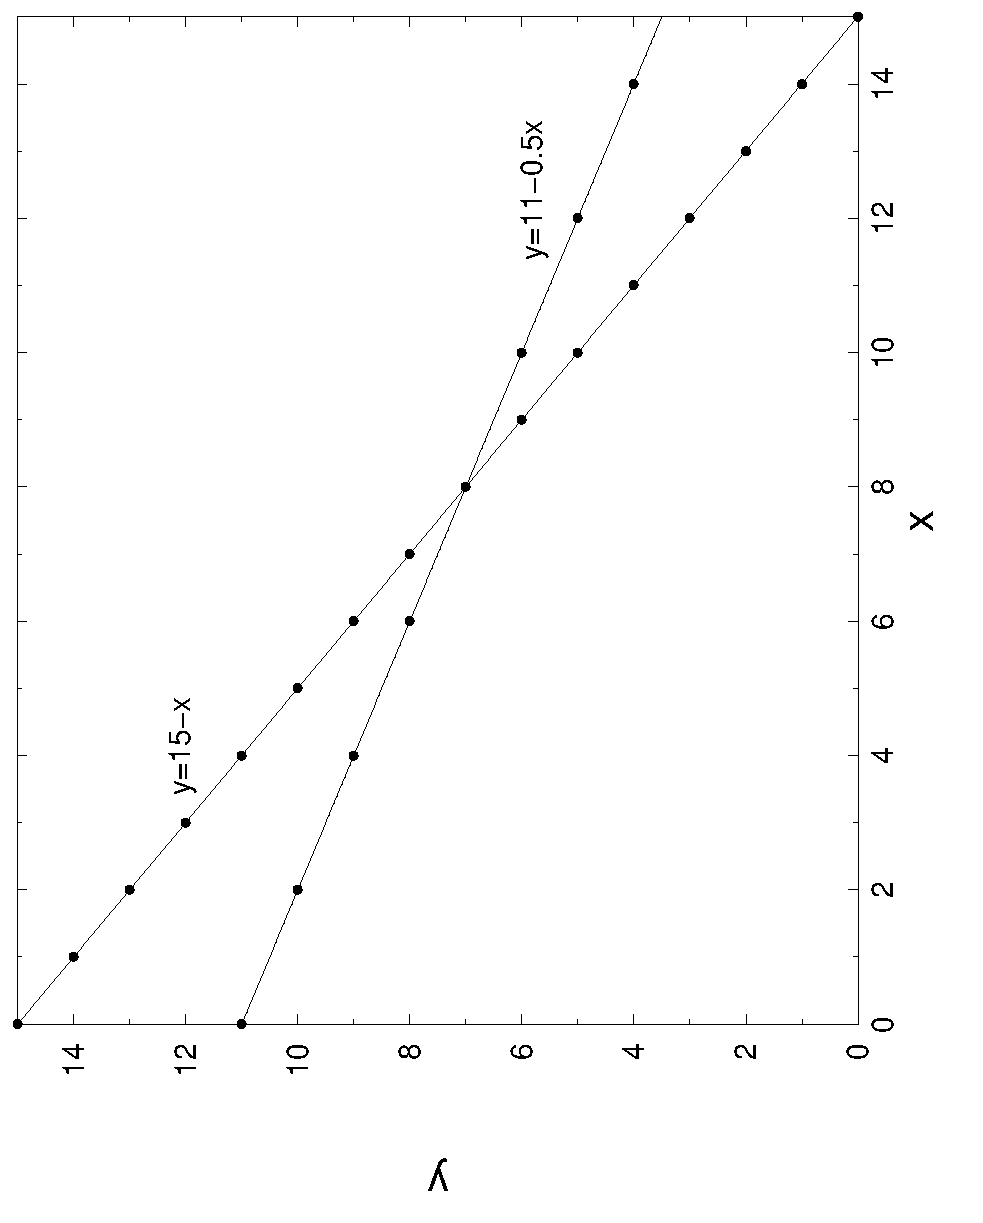
\includegraphics[angle=-90,width=\columnwidth]{pictures/augenbeine.eps}
  \caption{Im Koordinatensystem sind jeweils alle Punkte eingetragen, f\"ur welche die erste bzw. die zweite Gleichung erf\"ullt sind.}
  \label{fig:linglsyst:augenbeine}
\end{figure}

Wir sehen, dass sich f\"ur jede der beiden Gleichungen je eine Gerade ergibt, auf der die Punkte liegen. Klar: beide Gleichungen sind linear. Sie haben die Form
\begin{displaymath}
  y = ax + b
\end{displaymath}
n\"amlich:
\begin{eqnarray*}
  y & = & -x+15 \\
  y & = & -\frac{1}{2}x+11
\end{eqnarray*}
Beide sind die Funktionsgleichungen linearer Funktionen. F\"ur die erste Gleichung ist die Steigung $a=-1$ und der $y$-Achsenabschnitt $b=15$. F\"ur die zweite Gleichung ist $a=-\frac{1}{2}$ und $b=11$. Die beiden Geraden in \ref{fig:linglsyst:augenbeine} weisen tats\"achlich diese Eigenschaften auf.

F\"ur jeden Punkt einer Gerade ist jeweils die zugeh\"orige Funktionsgleichung erf\"ullt. An einem Punkt schneiden sich die beiden Geraden. F\"ur ihn sind beide Funktionsgleichungen erf\"ullt. Er entspricht deshalb der L\"osung des Gleichungssystems. Welcher Punkt ist es? Es ist $(x|y)=(8|7)$. Das ist genau das, was wir nun schon zweimal gefunden haben: F\"ur $x=8$ und $y=7$ sind beide Gleichungen (d.h. das Gleichungssystem) erf\"ullt.

Dieser Schnittpunkt k\"onnte allerdings auch so liegen, dass sich f\"ur $x$ oder f\"ur $y$ keine nat\"urliche Zahl ergibt. Dann w\"urde es keine Antwort geben, denn eine Anzahl von Tieren muss nun mal eine nat\"urliche Zahl sein.

Wir k\"onnen unser Problem also auch graphisch l\"osen. Jede Gleichung betrachten wir dann als Funktionsgleichung. Wenn wir die zugeh\"origen Graphen zeichnen, stellen wir alle Punkte dar, f\"ur welche die jeweiligen Gleichungen erf\"ullt sind. Im Schnittpunkt sind beide Gleichungen erf\"ullt. Dort liegt die L\"osung des Gleichungssystems.


\subsection{Lösung mit Cleverness suchen}
\label{linglsyst:raffiniert}

Gaby hat noch eine M\"oglichkeit gefunden, das Problem zu l\"osen:

	\begin{center}
	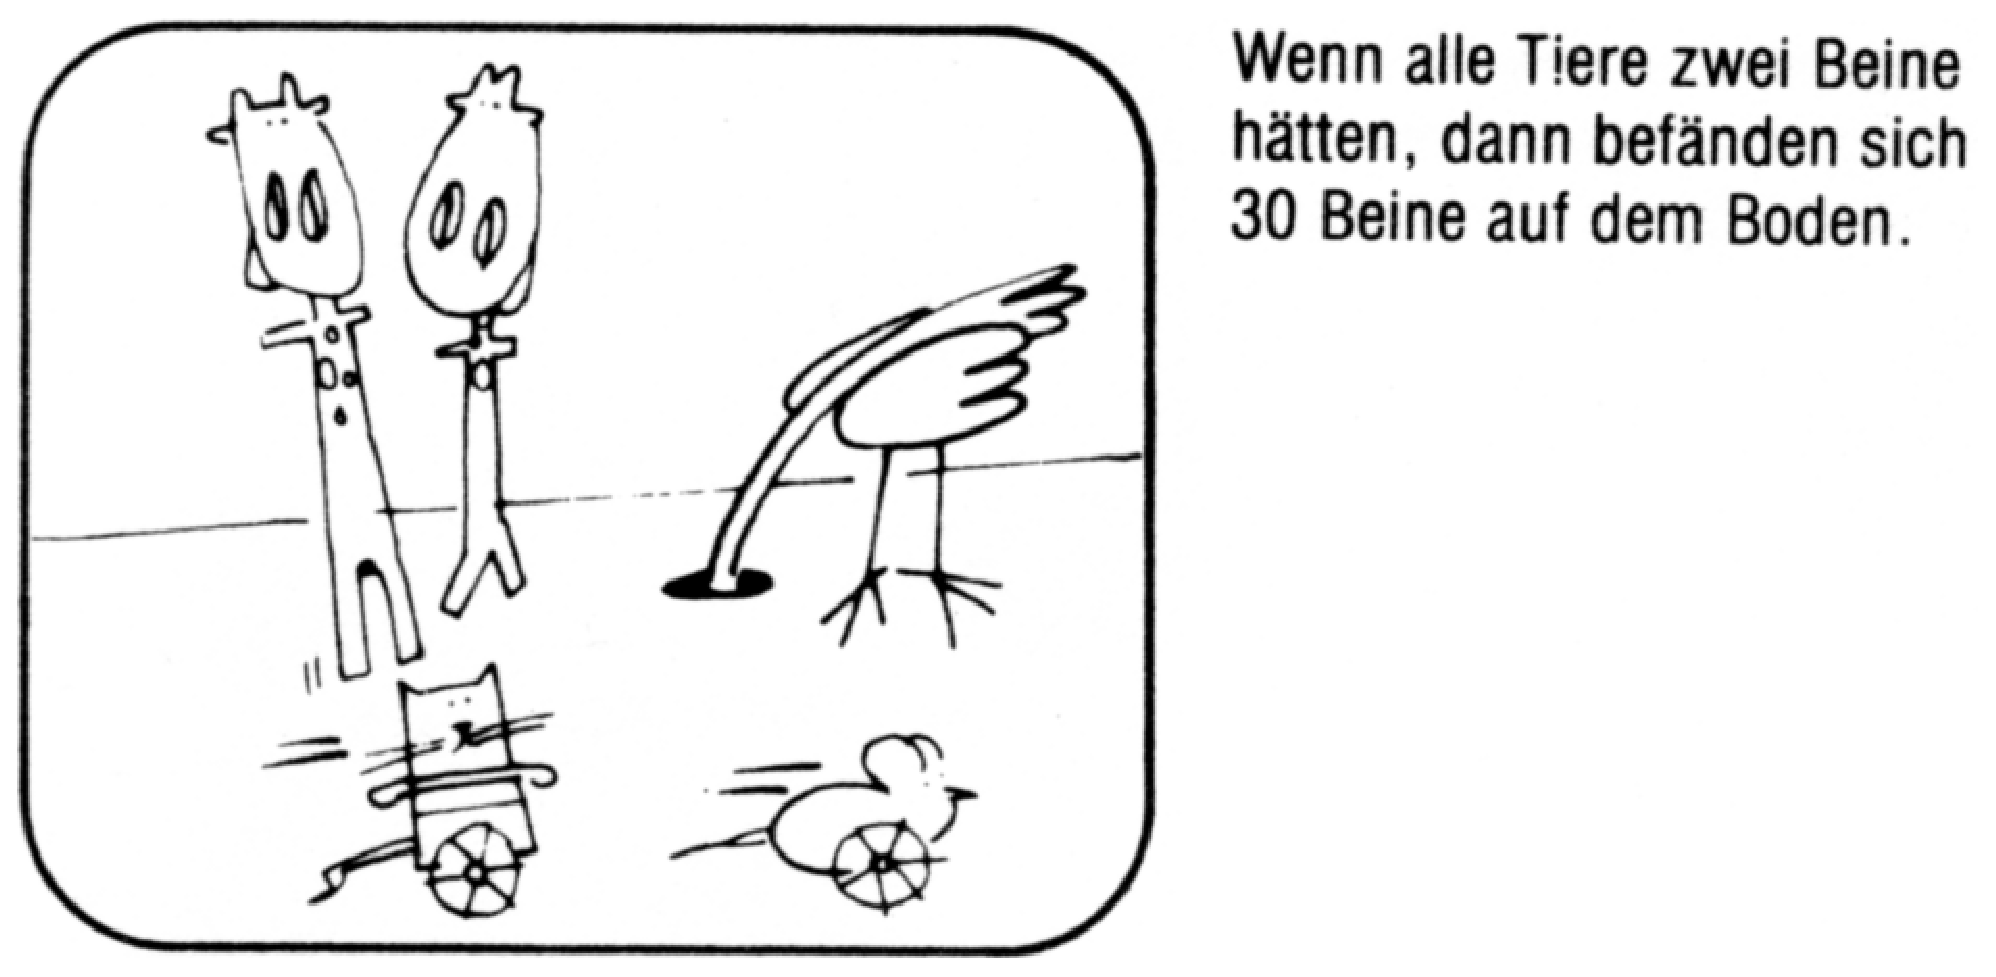
\includegraphics[width=0.9\columnwidth,bb=14 14 956 467]{pictures/augenbeine5t.eps}

	\medskip
	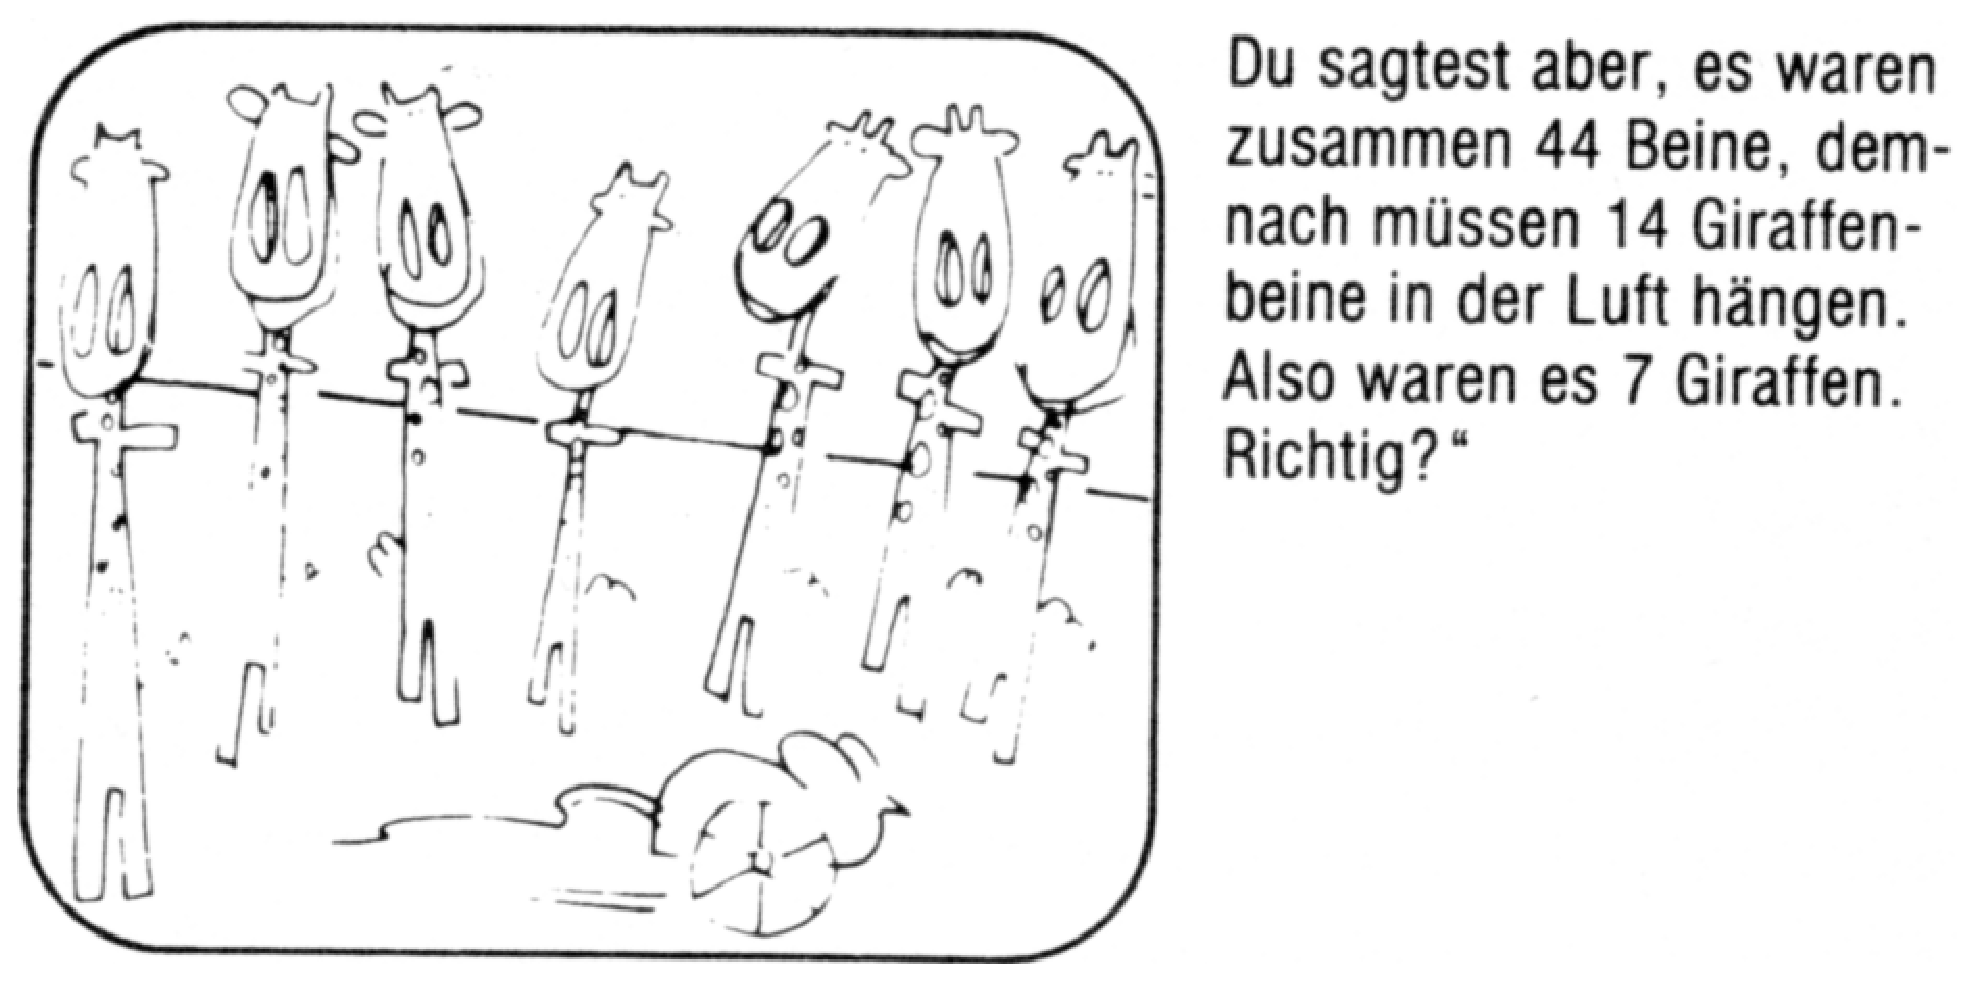
\includegraphics[width=0.9\columnwidth,bb=14 14 946 470]{pictures/augenbeine6t.eps}

	\medskip
	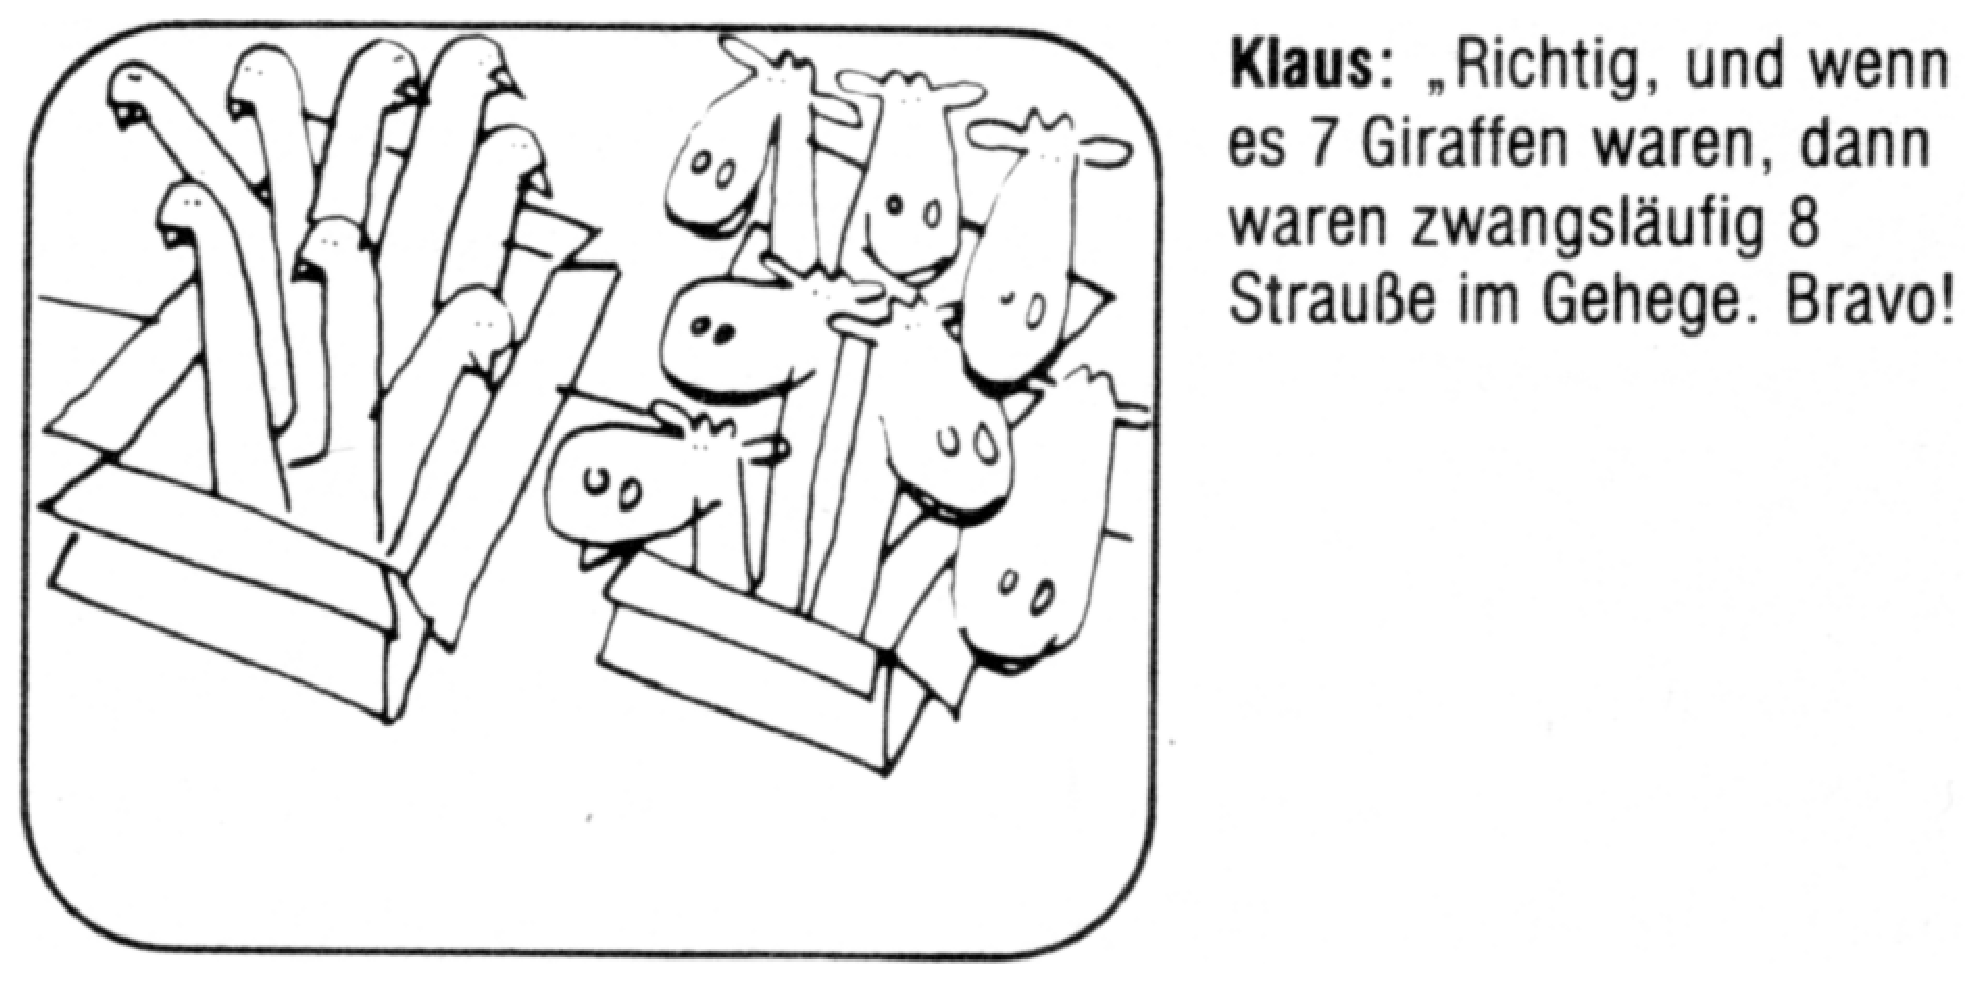
\includegraphics[width=\columnwidth,bb=14 14 950 470]{pictures/augenbeine7t.eps}
	\end{center}


Raffiniert! Aber wir werden wohl nicht immer eine so gute Idee haben, mit der wir das Problem l\"osen k\"onnen. Andererseits ist das Durchprobieren aller M\"oglichkeiten m\"uhsam. Und was ist, wenn $x$ und $y$ nicht Zahlen von Tieren sind, sondern Gr\"ossen, die grunds\"atzlich alle Zahlen als Werte annehmen k\"onnen. Wir k\"onnen doch nicht alle Zahlen durchprobieren! Dann bleibt uns noch die graphische Methode. Die w\"urde immer noch funktionieren. Allerdings ist sie nicht beliebig genau. Deshalb lernen wir eine weitere Methode kennen: die algebraische.

\subsection{Die algebraischen Methoden}
\label{linglsyst:algebraisch}

Schreiben wir das Gleichungssystem, das wir bereits bearbeitet haben, nochmals auf:
\begin{system}
  x+y & = & 15 \\
  2x+4y & = & 44
\end{system}Wenn wir an einer Gleichung eine \"Aqui"-valenzumformung durchf\"uhren, bleibt die L\"osungsmenge dieser Gleichung gleich. Damit \"andert aber auch die L\"osungsmenge des Gleichungssystems nicht. Denn diese ist die Schnittmenge der L\"osungsmengen der Einzelgleichungen. Wir d\"urfen also die Einzelgleichungen wie bisher umformen, wobei die bereits bekannten \"Aquivalenzumformungen erlaubt sind. Tats\"achlich haben wir das oben bereits getan.


\subsubsection{Die Einsetzungsmethode}
\label{linglsyst:algebraisch:einsetzung}

Wenn wir die erste Gleichung nach $y$ aufl\"osen, sieht das Gleichungssystem neu so aus:
\begin{system}
  y & = & 15-x \\
  2x+4y & = & 44
\end{system}

Die L\"osungsmenge dieses Gleichungssystems ist immer noch dieselbe wie jene des urspr\"unglichen. 

Die erste Gleichung sagt uns, dass $y$ gleich $15-x$ ist. Wir k\"onnen in der zweiten Gleichung also anstelle von $y$ ebenso gut $15-x$ schreiben, weil das dasselbe ist:
\begin{system}
  y & = & 15-x \\
  2x+4(15-x) & = & 44
\end{system}Wir haben die erste Gleichung in die zweite \emph{eingesetzt}. Dabei haben wir Klammern verwendet, damit das ganze $y$, d.h. $(15-x)$ mit 4 multipliziert wird.

Mit diesem Trick haben wir in der unteren Gleichung $y$ zum Verschwinden gebracht. Wir haben $y$ \emph{eliminiert}. Deshalb ist die zweite Gleichung zur einer gew\"ohnlichen linearen Gleichung mit einer einzigen Unbekannten, n\"amlich $x$, geworden. Wie man aus einer solchen Gleichung die L\"osung f\"ur $x$ herausholt, wissen wir bereits:
\begin{eqnarray*}
  2x+4(15-x) & = & 44 \\
  2x+60-4x & = & 44 \\
  60-2x & = & 44 \\
  -2x & = & -16 \\
  x & = & 8
\end{eqnarray*}
Dabei haben wir nur \"Aquivalenzumformungen durchgef\"uhrt. Wir k\"onnen deshalb anstelle der zweiten Gleichung auch die \"aquivalente Gleichung $x=8$ hinschreiben. Somit haben wir folgendes Gleichungssystem erhalten, dessen L\"osungsmenge immer noch gleich jener des urspr\"unglichen Systems ist:
\begin{system}
  y & = & 15-x \\
  x & = & 8
\end{system}Nun wissen wir, dass $x=8$ ist. Das k\"onnen wir seinerseits in die erste Gleichung einsetzen und finden so $y=15-8=7$:
\begin{system}
  y & = & 7 \\
  x & = & 8
\end{system}Bei unseren Umformungen haben wir die L\"o"-sungs"-men"-ge nie ver\"andert. Die L\"osung des urspr\"unglichen Gleichungssystems ist somit ebenfalls $x=8$ und $y=7$. Es sind immer noch 8 Strausse und 7 Giraffen.

Diesmal haben wir die L\"osung algebraisch gefunden. Diese Methode liefert uns immer das exakte Resultat, was die graphische Methode nicht leistet.

Einfache Aufgaben wie diese (mit den Straussen und Giraffen) haben wir \"ubrigens bereits fr\"uher nur mit einer einzigen Gleichung gel\"ost. Im obigen Beispiel h\"atten wir uns gesagt, $x$ sei die Zahl der Strausse. Dann ist $15-x$ die Zahl der Giraffen. Alle Strausse zusammen haben dann $2x$ Beine und die Giraffen $4(15-x)$ Beine. Zusammen m\"ussen das 44 Beine sein. Somit h\"atten wir dann die folgende Gleichung erhalten:
\begin{displaymath}
  2x + 4(15-x)=44
\end{displaymath}
Das ist genau die Gleichung, die wir weiter oben erhalten haben. Worin unterscheiden sich die beiden L\"osungsvarianten, d.h. was macht es f\"ur einen Unterschied, ob wir ein Gleichungssystem oder direkt eine einzige Gleichung aufstellen?
\begin{itemize}
\item Gleichungssystem mit $x$ und $y$: Die Giraffen-Zahl haben wir $y$ genannt. Die gesamt Tier-Zahl haben wir mit der Gleichung $x+y=15$ ausgedr\"uckt. Diese Gleichung haben wir nach $y$ aufgel\"ost ($y=15-x$) und in die andere Gleichung eingesetzt.
\item Eine Gleichung mit $x$: Wir haben der Giraffen-Zahl keinen eigenen Namen gegeben. Stattdessen haben wir sie als $15-x$ ausgedr\"uckt. Das ist aber dasselbe wie $y\,(=15-x)$. Wir haben gewissermassen die eine Gleichung $y=15-x$ direkt in die andere Gleichung eingesetzt, allerdings ohne die Bezeichnung $y$ zu verwenden.
\end{itemize}
Mit anderen Worten: eigentlich haben wir beide Male dasselbe getan, ausser dass wir in der Gleichungssystem-Variante f\"ur die Giraffen-Zahl einen eigenen Variablennamen gew\"ahlt haben.

Die Aufgaben, die sich uns stellen, sind aber nicht immer so einfach wie diese. Deshalb k\"onnen wir nicht immer sofort eine einzige Gleichung aufstellen, in welche die andere Gleichung bereits eingesetzt ist.


\subsubsection{Die Gleichsetzungsmethode}
\label{linglsyst:algebraisch:gleichsetzung}

Bei der graphischen Methode haben wir ebenfalls Gleichungen verwendet, die zu den urspr\"unglichen \"aquivalent sind. Wir haben einfach die beiden Gleichungen nach $y$ aufgel\"ost:
\begin{system}
  y & = & 15-x \\
  y & = & 11-\frac{1}{2}x
\end{system}
Wir haben sie als Funktionsgleichungen betrachtet, die Graphen gezeichnet und den Schnittpunkt gesucht. Dort sind n\"amlich f\"ur ein und dasselbe $x$ die zugeh\"origen $y$'s gleich.

Wir k\"onnen diese Methode auch algebraisch nachvollziehen. Wenn $y$ in beiden Gleichungen dasselbe sein soll, m\"ussen auch die rechten Seiten der Gleichungen gleich sein, weil sie ja beide gleich $y$ sind:
\begin{displaymath}
  15-x = 11-\frac{1}{2}x
\end{displaymath}
Damit haben wir durch Gleichsetzen eine lineare Gleichung mit einer einzigen Unbekannten erhalten, von der wir wissen, wie man sie l\"ost:
\begin{eqnarray*}
  15-x & = & 11-\frac{1}{2}x \\
  15 & = & 11 + \frac{1}{2}x \\
  4 & = & \frac{1}{2}x \\
  8 & = & x
\end{eqnarray*}
Auf diese Weise haben wir $x$ gefunden. Wie finden wir nun $y$? Ganz einfach: Wir haben ja zwei Gleichungen f\"ur $y$. Dort k\"onnen wir $x$ einsetzen:
\begin{eqnarray*}
  y & = & 15-x = 15-8 = 7 \\
  y & = & 11-\frac{1}{2}x = 11-\frac{1}{2}\cdot 8 =7
\end{eqnarray*}
Wir haben beide Male $y=7$ erhalten. Das muss nat\"urlich so sein. Sonst w\"aren ja die beiden Gleichungen gar nicht f\"ur dasselbe Paar $(x|y)=(8|7)$ erf\"ullt, und wir h\"atten es nicht mit einer L\"osung des Gleichungssystems zu tun. Es reicht also, wenn wir $x$ in eine der beiden Gleichungen einsetzen. Es sei denn, wir m\"ochten kontrollieren, ob wir einen Fehler gemacht haben.

Diese Gleichsetzungsmethode ist eigentlich eine Spezialform der Einsetzungsmethode. Denn wir setzen ja das, was wir in der ersten Gleichung f\"ur $y$ erhalten haben, in die zweite ein. Speziell ist nur, dass wir die zweite Gleichung auch nach $y$ aufgel\"ost haben.

Betrachten wir noch ein Beispiel:
\begin{system}
  28y-9 & = & 7x+15 \\
  28y-9 & = & 31x-5
\end{system}Die linke Seite ist f\"ur beide Gleichungen gleich. Deshalb m\"ussen auch die rechten Seiten gleich sein. Wir k\"onnen sie deshalb gleichsetzen:
\begin{eqnarray*}
  7x+15 & = & 31x-5 \\
  15 & = & 24x - 5 \\
  20 & = & 24x \\
  x & = & \frac{20}{24}=\frac{5}{6}
\end{eqnarray*}
$y$ erhalten wir, indem wir $x$ in eine der beiden Ausgangsgleichungen einsetzen, z.B. in die erste:
\begin{eqnarray*}
  28y-9 & = & 7\cdot\frac{5}{6}+15 \\
  28y & = & \frac{35}{6} + 24 = \frac{35}{6}+\frac{144}{6} = \frac{179}{6} \\
  y & = & \frac{179}{168}
\end{eqnarray*}
Wir k\"onnen also nicht nur dann gleichsetzen, wenn beide Gleichungen nach einer Variablen (z.B. $y$) aufgel\"ost sind. Die Methode funktioniert immer, wenn beide Gleichungen eine Seite gemeinsam haben und auf der anderen Seite nur eine Variable steht.

\subsubsection{Das Additionsverfahren}

Es gibt noch weitere Möglichkeiten, die Lösungen algebraisch zu finden. Beim Additionsverfahren werden gegebenenfalls die Gleichungen so multipliziert, dass beim anschliessenden Addieren bzw. Subtrahieren einer Gleichung von der andern eine Variable $0$ ergibt. Es bleibt dann eine Gleichung mit nur einer Unbekannten übrig, die man leicht lösen kann. Natürlich würde man in folgendem Beispiel
\begin{system}
  y & = & 15-x \\
  y & = & 11-\frac{1}{2}x
\end{system}
gleichsetzen. Ich möchte an dieser Stelle aber das Additionsverfahren demonstrieren und werde die Variable $x$ eliminieren.

Aus der zweiten Gleichung folgt mit Multiplikation mit $2$
$$2y = 22 - x.$$
Jetzt kann man von der ersten Gleichung die zweite subtrahieren
\begin{system}
  y & = & 15-x \\
  2y & = & 22-x
\end{system}
wobei $-x-(-x)=0$ und erhält also
$$-y = -7$$
das heisst $y=7$. Es folgt unmittelbar $x=8$.


\subsection{Verschiedene F\"alle}
\label{linglsyst:faelle}

L\"osen wir nun folgendes Gleichungssystem:
\begin{system}
  y+2 & = & 3x \\
  2y & = & 6x+1
\end{system}Dabei verwenden wir die Einsetzungsmethode. Zuerst l\"osen wir die erste Gleichung nach $y$ auf:
\begin{system}
  y & = & 3x-2 \\
  2y & = & 6x+1
\end{system}Dann setzen wir die erste Gleichung in die zweite ein und l\"osen diese:
\begin{eqnarray*}
  2(3x-2) & = & 6x+1 \\
  6x-4 & = & 6x+1 \\
  6x & = & 6x + 5 \\
  x & = & x + \frac{5}{6}
\end{eqnarray*}
Diese Gleichung hat keine L\"osung. Wenn wir zu einer Zahl $\frac{5}{6}$ addieren, erhalten wir mehr als diese Zahl. Die Gleichung ist deshalb f\"ur kein $x$ erf\"ullbar.\footnote{Wir h\"atten in der zweitletzten Zeile auch auf beiden Seiten $6x$ subtrahieren k\"onnen und h\"atten $0=5$ erhalten. Das ist eine falsche Aussage, unabh\"angig davon was $x$ ist. Deshalb gibt es keine L\"osung f\"ur $x$. Weil die erste Gleichung \"aquivalent zur Gleichung $0=5$ ist, hat auch sie keine L\"osung.}

Das betrachtete Gleichungssystem hat keine L\"osung. Das k\"onnen wir graphisch veranschaulichen. Daf\"ur l\"osen wir beide Gleichungen nach $y$ auf:
\begin{system}
  y & = & 3x-2 \\
  y & = & 3x+\frac{1}{2}
\end{system}Diese Gleichungen k\"onnen wir als Funktionsgleichungen betrachten. In \ref{fig:linglsyst:parallel} sind die beiden Graphen gezeichnet.

\begin{figure}[t!]
  \centering
  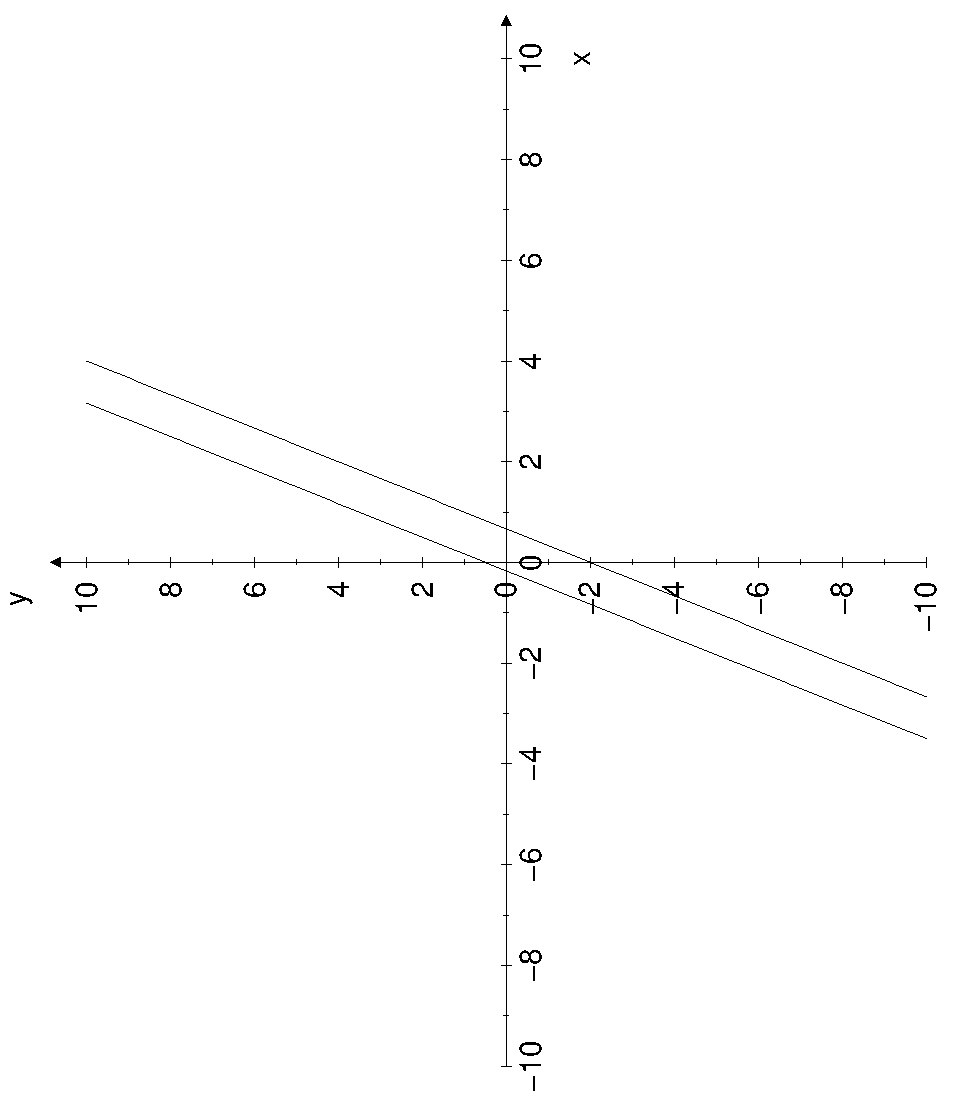
\includegraphics[angle=-90,width=0.9\columnwidth]{pictures/parallel.eps}
  \caption{Die Graphen der Funktionen $y=3x-2$ und $y=3x+\frac{1}{2}$ sind parallel, denn sie haben dieselbe Steigung.}
  \label{fig:linglsyst:parallel}
\end{figure}

Die beiden Geraden sind parallel. Das ist klar, denn beide haben die Steigung 3. Und Geraden mit gleicher Steigung sind nun mal parallel. Deshalb schneiden sie sich nicht. Und weil der Schnittpunkt die L\"osung des Gleichungssystems w\"are, gibt es keine L\"osung.

Mit Hilfe der graphischen Methode wird klar, welche M\"oglichkeiten es f\"ur die L\"osungsmenge eines Gleichungssystems gibt:
\begin{itemize}
\item Entweder schneiden sich die beiden Geraden in einem Punkt. Dann gibt es genau eine L\"osung --- nicht mehr und nicht weniger. Diese L\"osung entspricht dem Schnittpunkt.
\item Die Geraden sind parallel. Dann gibt es keinen Schnittpunkt und somit keine L\"osung.
\item Die beiden Geraden liegen aufeinander, d.h. sie sind identisch. Dann gibt es unendlich viele Schnittpunkte und somit unendlich viele L\"osungen.
\end{itemize}

Betrachten wir ein weiteres Beispiel:
\begin{system}
  2y-4x & = & 6 \\
  6x & = & 3y-9
\end{system}Wir l\"osen die erste Gleichung nach $y$ auf:
\begin{eqnarray*}
  2y-4x & = & 6 \\
  2y & = & 6+4x \\
  y & = & 3+2x
\end{eqnarray*}
Dann setzen wir sie in die zweite Gleichung ein:
\begin{eqnarray*}
  6x & = & 3(3+2x)-9 \\
  6x & = & 9+6x-9 \\
  6x & = & 6x
\end{eqnarray*}
Diese Gleichung ist f\"ur jedes $x$ erf\"ullt. Zu jedem $x$ k\"onnen wir dann mit Hilfe der ersten Gleichung $y=3+2x$ das zugeh\"orige $y$ berechnen. So erhalten wir unendlich viele Paare $(x|y)$, die alle L\"osungen des Gleichungssystems sind. Die L\"osungsmenge enth\"alt also alle Paare $(x|y)$, die gem\"ass der Gleichung $y=3+2x$ zusammenh\"angen:\footnote{Dabei verwenden wir die beschreibende Mengenschreibweise: Der Raum zwischen den geschweiften Klammern wird durch den senkrechten Strich in zwei Abschnitte unterteilt: Das Paar $(x|y)$ vor dem $|$ steht f\"ur ein beliebiges Element der Menge. Hinter dem $|$ stehen die Bedingungen, die jedes $(x|y)$-Paar erf\"ullen muss, damit es zur Menge geh\"ort.}
\begin{displaymath}
  L=\{(x|y)\,|\,x\in\mathbb{R}, y=3+2x\}
\end{displaymath}

Wir haben die erste Gleichung nach $y$ aufgel\"ost. Wenn wir die zweite Gleichung ebenfalls nach $y$ aufl\"osen, sehen wir Folgendes:
\begin{eqnarray*}
  6x & = & 3y-9 \\
  6x+9 & = & 3y \\
  2x+3 & = & y
\end{eqnarray*}
Das ist genau dieselbe (Funktions-)Gleichung wie die erste. Deshalb ergibt sich als Graph dieselbe Gerade. Weil beide Geraden identisch sind, gibt es unendlich viele Schnittpunkte und somit ebenso viele L\"osungen. Definiert werden diese Schnittpunkte bzw. L\"osungen durch die (Funktions-)Gleichung $y=2x+3$.

Die beiden Gleichungen dieses Systems sind \"aquivalent. D.h. sie haben dieselbe L\"osungsmenge. Deshalb haben wir im Grunde nur eine Gleichung mit zwei Unbekannten. Bereits in Abschnitt \ref{linglsyst:heraussuchen} haben wir gesehen, dass es in diesem Fall viele L\"osungen gibt, da wir zu jedem $x$ ein zugeh\"origes $y$ finden, indem wir $y=3+2x$ berechnen. Damit zwei Unbekannte eindeutig bestimmt sind, ben\"otigen wir aber zwei Gleichungen, die wirklich verschieden sind.\footnote{Allerdings ist es bei zwei verschiedenen Gleichungen auch m\"oglich, dass es gar keine L\"osung gibt, wie wir oben gesehen haben.}

\section*{Übungen}

\begin{enumerate}

\item \label{aufg:linglsyst:graphisch} L\"osen Sie folgende Gleichungssysteme graphisch.
  \begin{enumerate}
  \item 
    \begin{system}
      y & = & x+1 \\
      y & = & -2x
    \end{system}
  \item 
    \begin{system}
      y & = & 2x-2 \\
      y & = & -\frac{1}{2}x+2
    \end{system}
  \item 
    \begin{system}
      x+y & = & 2 \\
      2x-y & = & 0
    \end{system}
  \item 
    \begin{system}
      3x+4y & = & -6 \\
      y & = & 3
    \end{system}
  \end{enumerate}

\item \label{aufg:linglsyst:einsetzung} L\"osen Sie folgende Gleichungssysteme mit der Einsetzungsmethode:
  \begin{enumerate}
  \item 
    \begin{system}
      y-x & = & 12 \\
      y & = & 2x+5
    \end{system}
  \item 
    \begin{system}
      x & = & 2y \\
      x+3y & = & 10
    \end{system}
  \item 
    \begin{system}
      x+y & = & 8 \\
      3x-2y & = & 14
    \end{system}
  \item 
    \begin{system}
      x+y & = & 5(a+b) \\
      y & = & x-a+b
    \end{system}
  \end{enumerate}

\item \label{aufg:linglsyst:gleichsetzung} L\"osen Sie folgende Gleichungssysteme mit der Gleichsetzungsmethode:
  \begin{enumerate}
  \item 
    \begin{system}
      y & = & 5x-50 \\
      y & = & -x+10
    \end{system}
  \item 
    \begin{system}
      x & = & 2y+1 \\
      x & = & 4y-3
    \end{system}
  \item 
    \begin{system}
      y & = & 3x \\
      2y & = & 5x+3
    \end{system}
  \item 
    \begin{system}
      5y-2 & = & 3x-3 \\
      5y-2 & = & -4x+11
    \end{system}
  \item 
    \begin{system}
      y & = & ax+b \\
      y & = & -ax-b
    \end{system}
  \end{enumerate}


\item L\"osen Sie folgende Gleichungssysteme algebraisch:
  \begin{enumerate}
  \item 
    \begin{displaymath}
      \left| 
        \begin{array}{rcl}
          200x & = & y \\
          10x+y & = & 21
        \end{array} \right|
    \end{displaymath}

  \item 
    \begin{displaymath}
      \left| 
        \begin{array}{rcl}
         x+y & = & 8.45 \\
         x-y & = & 3.23
        \end{array} \right|
    \end{displaymath}

  \item 
    \begin{displaymath}
      \left| 
        \begin{array}{rcl}
         0.1x + 0.2y & = & 3 \\
         0.2x - 0.1y & = & 1
        \end{array} \right|
    \end{displaymath}

  \item 
    \begin{displaymath}
      \left| 
        \begin{array}{rcl}
         9x-2y & = & 31 \\
         7x+6y & = & 77
        \end{array} \right|
    \end{displaymath}

  \item 
    \begin{displaymath}
      \left| 
        \begin{array}{rcl}
         2x+3y & = & 98 \\
         4x-y & = & 98
        \end{array} \right|
    \end{displaymath}

  \item 
    \begin{displaymath}
      \left| 
        \begin{array}{rcl}
         y & = & 3x-11 \\
         y & = & 13-5x
        \end{array} \right|
    \end{displaymath}

  \item 
    \begin{displaymath}
      \left| 
        \begin{array}{rcl}
         1200x + 1500y & = & 27000 \\
         0.2x-0.1y & = & 1
        \end{array} \right|
    \end{displaymath}

  \item 
    \begin{displaymath}
      \left| 
        \begin{array}{rcl}
         y & = & 3x \\
         3x-y & = & 0
        \end{array} \right|
    \end{displaymath}

  \item 
    \begin{displaymath}
      \left| 
        \begin{array}{rcl}
        x+3y & = & 1.1 \\
        3x+y & = & 0.9
        \end{array} \right|
    \end{displaymath}

  \item 
    \begin{displaymath}
      \left| 
        \begin{array}{rcl}
         y-5x & = & 7 \\
          y & = & 6+5x
        \end{array} \right|
    \end{displaymath}

  \item 
    \begin{displaymath}
      \left| 
        \begin{array}{rcl}
         5x & = & 1-3y \\
         5x & = & 3y+\frac{1}{4}
        \end{array} \right|
    \end{displaymath}

  \item 
    \begin{displaymath}
      \left| 
        \begin{array}{rcl}
         \frac{x-7}{y-2} & = & \frac{1}{4} \\
          \frac{x}{y} & = & \frac{5}{7}
        \end{array} \right|
    \end{displaymath}

  \item 
    \begin{displaymath}
      \left| 
        \begin{array}{rcl}
         5x-3y & = & 6 \\
         4x & = & 2y+6
        \end{array} \right|
    \end{displaymath}

  \item 
    \begin{displaymath}
      \left| 
        \begin{array}{rcl}
         28y-9 & = & 7x+15 \\
         31x-5 & = & 28y-9
        \end{array} \right|
    \end{displaymath}


  \item 
    \begin{displaymath}
      \left| 
        \begin{array}{rcl}
         \frac{x+y}{x-y} & = & \frac{a+b}{a-b} \\
          3x-2y & = & 3a - 2b
        \end{array} \right|
    \end{displaymath}

  \item 
    \begin{displaymath}
      \left| 
        \begin{array}{rcl}
         x-5y & = & 7 \\
         x & = & 5y+7
        \end{array} \right|
    \end{displaymath}

  \item 
    \begin{displaymath}
      \left| 
        \begin{array}{rcl}
         -4x+6y & = & 5 \\
         6x-9y & = & -8
        \end{array} \right|
    \end{displaymath}

  \item 
    \begin{displaymath}
      \left| 
        \begin{array}{rcl}
         ax+y & = & 1 \\
         x+by & = & 1
        \end{array} \right|
    \end{displaymath}

  \item 
    \begin{displaymath}
      \left| 
        \begin{array}{rcl}
         mx+cy & = & a+b \\
         mx & = & (a-c)y
        \end{array} \right|
    \end{displaymath}

  \item 
    \begin{displaymath}
      \left| 
        \begin{array}{rcl}
         x-y & = & d \\
         \frac{x-y}{2}+dx & = & d
        \end{array} \right|
    \end{displaymath}




  \end{enumerate}

\item Die Preise f\"ur das Auslegen von Bodenplatten zweier Firmen berechnen sich wie folgt:
  \begin{itemize}
  \item Firma A: Grundpreis: 600\unit{Fr.} \qquad Quadratmeterpreis: 105\ufrac{Fr.}{m^2}
  \item Firma B: Grundpreis: 400\unit{Fr.} \qquad Quadratmeterpreis: 115\ufrac{Fr.}{m^2}
  \end{itemize}
    \begin{enumerate}
    \item Geben Sie f\"ur beide Firmen die Funktionsgleichung an, mit der wir den Preis aus der Bodenfl\"ache berechnen k\"onnen.
    \item Zeichnen Sie die zugeh\"origen Funktionsgraphen (bis zu einer Fl\"ache von $\unit[40]{m^2}$ f\"ur beide Firmen in dasselbe Diagramm.
    \item In welchem Bereich ist Firma A bzw. Firma B billiger? (L\"osung graphisch und algebraisch)
    \end{enumerate}

\item Zwei Z\"uge starten genau um 12:00 Uhr in Bern und Z\"urich und fahren einander entgegen. Der Zug aus Z\"urich f\"ahrt 120\ufrac{km}{h}, derjenige aus Bern nur 90\ufrac{km}{h}. Von Bern bis Z\"urich sind es 144 Bahnkilometer.
  \begin{enumerate}
  \item Geben Sie f\"ur beide Z\"uge die Funktionsgleichung an, mit der wir die Entfernung von Bern aus der Zeit seit dem Start berechnen k\"onnen.
  \item Zeichnen Sie die zugeh\"origen Funktionsgraphen f\"ur beide Z\"uge ins selbe Diagramm.
  \item Wann und wie weit von Bern entfernt treffen sich die beiden Z\"uge? (L\"osung graphisch und algebraisch)
  \end{enumerate}

\item L\"osen Sie folgende Aufgaben mithilfe von Gleichungssystemen:
  \begin{enumerate}
  \item Eine Firma verteilt ihre 57 Mitarbeiterinnen und Mitarbeiter auf zw\"olf Filialen. Wie viele Filialen erhalten f\"unf und wie viele nur vier Mitarbeiter/innen? Stellen Sie Gleichungen auf und l\"osen Sie sie.
    
  \item Wir m\"ochten ein Dach mit einer Fl\"ache von $\unit[165]{m^2}$ mit einer m\"oglichst grossfl\"achigen Solaranlage bedecken, soweit das Budget von 28500 Franken reicht. Den Rest der Fl\"ache bedecken wir mit normalen Ziegeln. Wie gross sind die Fl\"achen, die wir mit Solarpanels bzw. mit Ziegeln bedecken k\"onnen, wenn die Solarpanels (inkl. Installation) $\unit[242]{Fr.}$ pro $\unit{m^2}$ kosten und die Ziegel $\unit[105]{Fr.}$ pro $\unit{m^2}$?
    
  \item Wir haben zwei Sorten Bodenplatten eingekauft. Von der teuereren sind es 165 St\"uck, von der billigeren 245. Insgesamt haben wir 5929 Franken und 50 Rappen daf\"ur ausgegeben. F\"ur die Buchhaltung m\"ussen wir nun rekonstruieren, wie teuer die beiden Plattentypen pro St\"uck waren, weil wir es leider nirgends notiert haben und die Firma, von der wir die Platten gekauft haben, Betriebsferien hat. Immerhin k\"onnen wir uns daran erinnern, dass die billigeren Platten pro St\"uck genau 5 Franken weniger gekostet haben als die teureren.

\item Eine Landwirtin besitzt zwei Klee-Gras-Mischungen:
  \begin{itemize}
  \item Mischung 1: 50\% Klee- und 50\% Grassamen
  \item Mischung 2: 75\% Klee- und 25\% Grassamen
  \end{itemize}
  Sie muss 10\unit{kg} Klee- und 8\unit{kg} Grassamen s\"aen. Wieviel von jeder Mischung muss sie nehmen?

\item Ein Turnverein macht einen Ausflug. Der Car kostet 368\unit{Fr.} Auf die Reise gehen 15 Aktive und 13 G\"aste. Die G\"aste sollen 4\unit{Fr.} weniger zahlen als die Aktiven. Wie hoch m\"ussen die Preise f\"ur die Aktiven und die G\"aste gew\"ahlt werden, damit die Carkosten gedeckt werden?

\item Ein Luftschiff legt bei R\"uckenwind in der Stunde 90.4\unit{km} (gegen\"uber der Landschaft) zur\"uck, gegen den Wind jedoch nur 65.2\unit{km}. Wie gross sind die Windgeschwindigkeit und die Geschwindigkeit des Luftschiffs gegen\"uber der Luft.
\end{enumerate}

\end{enumerate}


\section*{L\"osungen}

\begin{enumerate}

\item 

\begin{center}
\definecolor{ccqqqq}{rgb}{0.8,0,0}
\definecolor{qqwuqq}{rgb}{0,0.39215686274509803,0}
\scalebox{0.618}{
\begin{tikzpicture}[line cap=round,line join=round,>=triangle 45,x=1cm,y=1cm]
\begin{axis}[
x=1cm,y=1cm,
axis lines=middle,
ymajorgrids=true,
xmajorgrids=true,
xmin=-8.0,
xmax=9.2,
ymin=-4.8,
ymax=6.9,
xtick={-7,-6,...,9},
ytick={-5,-4,...,6},]
\clip(-8.3,-5.3) rectangle (9.6,6.9);
\draw[line width=2pt,color=qqwuqq,smooth,samples=100,domain=-8.16:9.40] plot(\x,{(\x)+1});
\draw[line width=2pt,color=ccqqqq,smooth,samples=100,domain=-8.16:9.40] plot(\x,{(-2)*(\x)});
\begin{scriptsize}
\draw[color=qqwuqq] (-6.72,-3.73) node {$f$};
\draw[color=ccqqqq] (-4.22,5.79) node {$g$};
\draw[color=black] (8.8,0.3) node {$x$};
\draw[color=black] (-0.4,6.5) node {$y$};
\end{scriptsize}
\end{axis}
\end{tikzpicture}
}
\end{center}

  \begin{enumerate}
  \item
    \begin{displaymath}
      \result{(x|y) = \left(-\frac{1}{3}|\frac{2}{3}\right)}
    \end{displaymath}

  \item 
  
  \begin{center}
\definecolor{ccqqqq}{rgb}{0.8,0,0}
\definecolor{qqwuqq}{rgb}{0,0.39215686274509803,0}
\scalebox{0.618}{
\begin{tikzpicture}[line cap=round,line join=round,>=triangle 45,x=1cm,y=1cm]
\begin{axis}[
x=1cm,y=1cm,
axis lines=middle,
ymajorgrids=true,
xmajorgrids=true,
xmin=-8.0,
xmax=9.2,
ymin=-4.8,
ymax=6.9,
xtick={-7,-6,...,9},
ytick={-5,-4,...,6},]
\clip(-8.3,-5.3) rectangle (9.6,6.9);
\draw[line width=2pt,color=qqwuqq,smooth,samples=100,domain=-8.16:9.40] plot(\x,{2*(\x)-2});
\draw[line width=2pt,color=ccqqqq,smooth,samples=100,domain=-8.16:9.40] plot(\x,{(-0.5)*(\x)+2});
\begin{scriptsize}
\draw[color=qqwuqq] (-6.72,-3.73) node {$f$};
\draw[color=ccqqqq] (-4.22,5.79) node {$g$};
\draw[color=black] (8.8,0.3) node {$x$};
\draw[color=black] (-0.4,6.5) node {$y$};
\end{scriptsize}
\end{axis}
\end{tikzpicture}
}
\end{center}
  
    \begin{displaymath}
      \result{(x|y) = (1.6|1.2)}
    \end{displaymath}
  \item Zuerst l\"osen wir beide Gleichungen nach $y$ auf:
    \begin{displaymath}
      \left| 
        \begin{array}{rcl}
          y & = & 2-x \\
          y & = & 2x
        \end{array} \right|
    \end{displaymath}
    
    \begin{center}
\definecolor{ccqqqq}{rgb}{0.8,0,0}
\definecolor{qqwuqq}{rgb}{0,0.39215686274509803,0}
\scalebox{0.618}{
\begin{tikzpicture}[line cap=round,line join=round,>=triangle 45,x=1cm,y=1cm]
\begin{axis}[
x=1cm,y=1cm,
axis lines=middle,
ymajorgrids=true,
xmajorgrids=true,
xmin=-8.0,
xmax=9.2,
ymin=-4.8,
ymax=6.9,
xtick={-7,-6,...,9},
ytick={-5,-4,...,6},]
\clip(-8.3,-5.3) rectangle (9.6,6.9);
\draw[line width=2pt,color=qqwuqq,smooth,samples=100,domain=-8.16:9.40] plot(\x,{(-1)*(\x)+2});
\draw[line width=2pt,color=ccqqqq,smooth,samples=100,domain=-8.16:9.40] plot(\x,{(2)*(\x)});
\begin{scriptsize}
\draw[color=qqwuqq] (-6.72,-3.73) node {$f$};
\draw[color=ccqqqq] (-4.22,5.79) node {$g$};
\draw[color=black] (8.8,0.3) node {$x$};
\draw[color=black] (-0.4,6.5) node {$y$};
\end{scriptsize}
\end{axis}
\end{tikzpicture}
}
\end{center}

    \begin{displaymath}
      \result{(x|y) = \left(\frac{2}{3}|\frac{4}{3}\right)}
    \end{displaymath}
  \item Die erste Gleichung m\"ussen wir nach $y$ aufl\"osen:
    \begin{displaymath}
      \left| 
        \begin{array}{rcl}
          y & = & -\frac{3}{4}x-\frac{3}{2} \\
          y & = & 3
        \end{array} \right|
    \end{displaymath}
    
%\vspace{-20pt}
\begin{center}
\definecolor{ccqqqq}{rgb}{0.8,0,0}
\definecolor{qqwuqq}{rgb}{0,0.39215686274509803,0}
\scalebox{0.618}{
\begin{tikzpicture}[line cap=round,line join=round,>=triangle 45,x=1cm,y=1cm]
\begin{axis}[
x=1cm,y=1cm,
axis lines=middle,
ymajorgrids=true,
xmajorgrids=true,
xmin=-8.0,
xmax=9.2,
ymin=-4.8,
ymax=6.9,
xtick={-7,-6,...,9},
ytick={-5,-4,...,6},]
\clip(-8.3,-5.3) rectangle (9.6,6.9);
\draw[line width=2pt,color=qqwuqq,smooth,samples=100,domain=-8.16:9.40] plot(\x,{(-0.75)*(\x)-1.5});
\draw[line width=2pt,color=ccqqqq,smooth,samples=100,domain=-8.16:9.40] plot(\x,{3});
\begin{scriptsize}
\draw[color=qqwuqq] (-6.72,-3.73) node {$f$};
\draw[color=ccqqqq] (-4.22,5.79) node {$g$};
\draw[color=black] (8.8,0.3) node {$x$};
\draw[color=black] (-0.4,6.5) node {$y$};
\end{scriptsize}
\end{axis}
\end{tikzpicture}
}
\end{center}
    
    \begin{displaymath}
      \result{(x|y) = (-6|3)}
    \end{displaymath}
  \end{enumerate}
  
\item
  \begin{enumerate}
  \item 
    \begin{displaymath}
      \left| 
        \begin{array}{rcl}
          y-x & = & 12 \\
          y & = & 2x+5
        \end{array} \right|
    \end{displaymath}
    Die zweite Gleichung in die erste einsetzen und diese nach $x$ aufl\"osen:
    \begin{eqnarray*}
      2x+5-x & = & 12 \\
      x & = & 7
    \end{eqnarray*}
    $x$ in die zweite Gleichung einsetzen:
    \begin{displaymath}
      y = 2 \cdot 7 + 5 = 19
    \end{displaymath}
    L\"osung: $\result{(x|y)=(7|19)}$
    
  \item 
    \begin{displaymath}
      \left| 
        \begin{array}{rcl}
          x & = & 2y \\
          x+3y & = & 10
        \end{array} \right|
    \end{displaymath}
    Die erste Gleichung in die zweite einsetzen und diese nach $y$ aufl\"osen:
    \begin{eqnarray*}
      2y + 3y & = & 10 \\
      5y & = & 10 \\
      y & = & 2
    \end{eqnarray*}
    $y$ in die erste Gleichung einsetzen:
    \begin{displaymath}
      x = 2 \cdot 2 = 4
    \end{displaymath}
    L\"osung: $\result{(x|y)=(4|2)}$

  \item 
    \begin{displaymath}
      \left| 
        \begin{array}{rcl}
          x+y & = & 8 \\
        3x-2y & = & 14
      \end{array} \right|
  \end{displaymath}
  Die erste Gleichung z.B. nach $x$ aufl\"osen:
  \begin{displaymath}
    \left| 
      \begin{array}{rcl}
        x & = & 8-y \\
        3x-2y & = & 14
      \end{array} \right|
  \end{displaymath}
  Die erste Gleichung in die zweite einsetzen und diese nach $y$ aufl\"osen:
  \begin{eqnarray*}
    3(8-y)-2y & = & 14 \\
    24-3y-2y & = & 14 \\
    -5y & = & -10 \\
    y & = & 2
  \end{eqnarray*}
    $y$ in die erste Gleichung ($x=8-y$) einsetzen:
    \begin{displaymath}
      x = 8-2 = 6
    \end{displaymath}
    L\"osung: $\result{(x|y)=(6|2)}$
    
  \item 
    \begin{displaymath}
      \left| 
        \begin{array}{rcl}
          x+y & = & 5(a+b) \\
          y & = & x-a+b
        \end{array} \right|
    \end{displaymath}
    Die zweite Gleichung in die erste einsetzen und diese nach $x$ aufl\"osen:
    \begin{eqnarray*}
      x + x-a+b & = & 5(a+b) \\
      2x -a+b & = & 5a+5b \\
      2x & = & 6a+4b \\
      x & = & 3a+2b
    \end{eqnarray*}
    $x$ in die zweite Gleichung einsetzen:
    \begin{displaymath}
      y = 3a+2b-a+b = 2a+3b
    \end{displaymath}
    L\"osung: $\result{(x|y)=(3a+2b|2a+3b)}$
  \end{enumerate}

\item 
  \begin{enumerate}
  \item 
    \begin{displaymath}
      \left| 
        \begin{array}{rcl}
          y & = & 5x-50 \\
          y & = & -x+10
        \end{array} \right|
    \end{displaymath}
    Die rechten Seiten gleichsetzen und nach $x$ aufl\"osen:
    \begin{eqnarray*}
      5x-50 & = & -x+10 \\
      6x & = & 60 \\
      x & = & 10
    \end{eqnarray*}
    $x$ z.B. in die erste Gleichung einsetzen:
    \begin{displaymath}
      y = 5 \cdot 10 - 50 = 0
    \end{displaymath}
    Evtl. $x$ zur Kontrolle in die zweite Gleichung einsetzen:
    \begin{displaymath}
      y = -10 + 10 = 0
    \end{displaymath}
    L\"osung: $\result{(x|y)=(10|0)}$

  \item 
    \begin{displaymath}
      \left| 
        \begin{array}{rcl}
          x & = & 2y+1 \\
          x & = & 4y-3
        \end{array} \right|
    \end{displaymath}
    Die rechten Seiten gleichsetzen und nach $y$ aufl\"osen:
    \begin{eqnarray*}
      2y+1 & = & 4y-3 \\
      4 & = & 2y \\
      y & = & 2
    \end{eqnarray*}
    $y$ z.B. in die erste Gleichung einsetzen:
    \begin{displaymath}
      x = 2 \cdot 2+1 = 5
    \end{displaymath}
    Evtl. zur Kontrolle $y$ in die zweite Gleichung einsetzen:
    \begin{displaymath}
      x = 4 \cdot 2 -3 = 5
    \end{displaymath}
    L\"osung: $\result{(x|y)=(5|2)}$

  \item 
    \begin{displaymath}
      \left| 
        \begin{array}{rcl}
          y & = & 3x \\
          2y & = & 5x+3
        \end{array} \right|
    \end{displaymath}
    Die erste Gleichung verdoppeln, damit die beiden linken Seiten gleich werden:
    \begin{displaymath}
      \left| 
        \begin{array}{rcl}
          2y & = & 6x \\
          2y & = & 5x+3
        \end{array} \right|
    \end{displaymath}  
    Die rechten Seiten gleichsetzen und nach $x$ aufl\"osen:
    \begin{eqnarray*}
      6x & = & 5x+3 \\
      x & = & 3
    \end{eqnarray*}
    $x$ in die urspr\"ungliche erste Gleichung einsetzen:
    \begin{displaymath}
      y = 3 \cdot 3 = 9
    \end{displaymath}
    L\"osung: $\result{(x|y)=(3|9)}$

  \item 
    \begin{displaymath}
      \left| 
        \begin{array}{rcl}
          5y-2 & = & 3x-3 \\
          5y-2 & = & -4x+11
        \end{array} \right|
    \end{displaymath}
    Die beiden linken Seiten sind gleich. Auf den rechten Seiten steht nur die Variable $x$. Deshalb k\"onnen wir die beiden rechten Seiten gleichsetzen und nach $x$ aufl\"osen:
    \begin{eqnarray*}
      3x-3 & = & -4x+11 \\
      7x & = & 14 \\
      x & = & 2
    \end{eqnarray*}
    Wir setzen $x$ z.B. in die erste Gleichung ein und l\"osen nach $y$ auf:
    \begin{eqnarray*}
      5y-2 & = & 3\cdot 2 - 3 = 3 \\
      5y & = & 5 \\
      y & = & 1
    \end{eqnarray*}
    L\"osung: $\result{(x|y)=(2|1)}$

  \item 
    \begin{displaymath}
      \left| 
        \begin{array}{rcl}
          y & = & ax+b \\
          y & = & -ax-b
        \end{array} \right|
    \end{displaymath}
    Beide rechten Seiten gleichsetzen und nach $x$ aufl\"osen:
    \begin{eqnarray*}
      ax+b & = & -ax-b \\
      2ax & = & -2b \\
      x & = & -\frac{b}{a}
    \end{eqnarray*}
    $x$ z.B. in die erste Gleichung einsetzen:
    \begin{displaymath}
      y = a\left(-\frac{b}{a}\right)+b = -b+b=0
    \end{displaymath}
    L\"osung: $\result{(x|y)=(-\frac{b}{a}|0)}$ ($a\neq 0$)

  \end{enumerate}


\item 
  \begin{enumerate}
  \item 
    \begin{displaymath}
      \left| 
        \begin{array}{rcl}
          200x & = & y \\
          10x+y & = & 21
        \end{array} \right|
    \end{displaymath}
    Einsetzungsmethode: Erste Gleichung in zweite einsetzen und nach $x$ aufl\"osen:
    \begin{eqnarray*}
      10x+200x & = & 21 \\
      210x & = & 21 \\
      x & = & \frac{1}{10}
    \end{eqnarray*}
    $x$ in die erste Gleichung einsetzen:
    \begin{displaymath}
      y = 200 \cdot \frac{1}{10}=20
    \end{displaymath}
    L\"osung: $\result{(x|y)=(\frac{1}{10}|20)}$
    
  \item 
    \begin{displaymath}
      \left| 
        \begin{array}{rcl}
          x+y & = & 8.45 \\
          x-y & = & 3.23
        \end{array} \right|
    \end{displaymath}
Gleichsetzungsmethode: beide Gleichungen nach $x$ aufl\"osen:
    \begin{displaymath}
      \left| 
        \begin{array}{rcl}
          x & = & 8.45-y \\
          x & = & 3.23+y
        \end{array} \right|
    \end{displaymath}
gleichsetzen:
\begin{eqnarray*}
8.45-y & = & 3.23+y \\
5.22 & = & 2y \\
2.61 & = & y \\
x & = & 3.23+y = 5.84
\end{eqnarray*}
    L\"osung: $\result{(x|y)=(5.84|2.61)}$

    oder: Einsetzungsmethode: Zweite Gleichung nach $x$ aufl\"osen ($x=3.23+y$), in die erste einetzen ($3.23+y+y=8.45$) und nach $y$ aufl\"osen. Dann $x$ mit der zweiten Gleichung ($x=3.23+y$) berechnen.

  \item 
    \begin{displaymath}
      \left| 
        \begin{array}{rcl}
         0.1x + 0.2y & = & 3 \\
         0.2x - 0.1y & = & 1
        \end{array} \right|
    \end{displaymath}
Beide Gleichungen mit 10 multiplizieren, um die Dezimalbr\"uche loszuwerden:
    \begin{displaymath}
      \left| 
        \begin{array}{rcl}
         x + 2y & = & 30 \\
         2x - y & = & 10
        \end{array} \right|
    \end{displaymath}
Einsetzungsmethode: erste Gleichung nach $x$ aufl\"osen:
\begin{displaymath}
x= 30-2y
\end{displaymath}
und in die zweite Gleichunge einsetzen:
\begin{eqnarray*}
2(30-2y)-y & = & 10 \\
60-4y-y & = & 10 \\
-5y & = & -50 \\
y & = & 10 \\
x & = & 30-2y=10
\end{eqnarray*}
    L\"osung: $\result{(x|y)=(10|10)}$

  \item 
    \begin{displaymath}
      \left| 
        \begin{array}{rcl}
         9x-2y & = & 31 \\
         7x+6y & = & 77
        \end{array} \right|
    \end{displaymath}
    Einsetzungsmethode: Erste Gleichung nach $y$ aufl\"osen:
    \begin{displaymath}
      \left| 
        \begin{array}{rcl}
         \frac{9x-31}{2} & = & y \\
         7x+6y & = & 77
        \end{array} \right|
    \end{displaymath}
    Erste Gleichung in die zweite einsetzen und nach $x$ aufl\"osen:
    \begin{eqnarray*}
      7x + 6 \cdot \frac{9x-31}{2} & = & 77 \\
      7x + 27x-93 & = & 77 \\
      34x & = & 170 \\
      x & = & 5
    \end{eqnarray*}
    $x$ in die erste Gleichung einsetzen:
    \begin{displaymath}
      y = \frac{9\cdot 5 - 31}{2} = 7
    \end{displaymath}
    L\"osung: $\result{(x|y)=(5|7)}$

  \item 
    \begin{displaymath}
      \left| 
        \begin{array}{rcl}
         2x+3y & = & 98 \\
         4x-y & = & 98
        \end{array} \right|
    \end{displaymath}
    Einsetzungsverfahren: Zweite Gleichung nach $y$ aufl\"osen:
    \begin{displaymath}
      \left| 
        \begin{array}{rcl}
         2x+3y & = & 98 \\
         4x-98 & = & y
        \end{array} \right|
    \end{displaymath}
    Zweite Gleichung in die erste einsetzen und nach $x$ aufl\"osen:
    \begin{eqnarray*}
      2x+3(4x-98) & = & 98 \\
      2x+12x-294 & = & 98 \\
      14x & = & 392 \\
      x & = & 28
    \end{eqnarray*}
    $x$ in die zweite Gleichung einsetzen und $y$ berechnen:
    \begin{displaymath}
      y = 4 \cdot 28 - 98 = 14
    \end{displaymath}
    L\"osung: $\result{(x|y)=(28|14)}$

  \item 
    \begin{displaymath}
      \left| 
        \begin{array}{rcl}
         y & = & 3x-11 \\
         y & = & 13-5x
        \end{array} \right|
    \end{displaymath}
    Gleichsetzungsverfahren: Die beiden rechten Seiten gleichsetzen und nach $x$ aufl\"osen:
    \begin{eqnarray*}
      3x-11 & = & 13-5x \\
      8x & = & 24 \\
      x & = & 3
    \end{eqnarray*}
    $x$ z.B. in die erste Gleichung einsetzen:
    \begin{displaymath}
      y = 3 \cdot 3 -11 = -2
    \end{displaymath}
    L\"osung: $\result{(x|y)=(3|-2)}$

  \item 
    \begin{displaymath}
      \left| 
        \begin{array}{rcl}
         1200x + 1500y & = & 27000 \\
         0.2x-0.1y & = & 1
        \end{array} \right|
    \end{displaymath}
Erste Gleichung durch 100 teilen (wird einfacher) und zweite Gleichung mit 10 multiplizieren, um die Dezimalbr\"uche loszuwerden:
    \begin{displaymath}
      \left| 
        \begin{array}{rcl}
         12x + 15y & = & 270 \\
         2x-y & = & 10
        \end{array} \right|
    \end{displaymath}
Zweite Gleichung nach $y$ aufl\"osen:
\begin{eqnarray*}
-y & = & 10-2x \\
y & = & 2x-10
\end{eqnarray*}
In die erste Gleichung einsetzen:
\begin{eqnarray*}
12x+15(2x-10) & = & 270 \\
12x+30x-150 & = & 270 \\
42x & = & 420 \\
x & = & 10 \\
y & = & 2x-10=10
\end{eqnarray*}
    L\"osung: $\result{(x|y)=(10|10)}$

  \item 
    \begin{displaymath}
      \left| 
        \begin{array}{rcl}
         y & = & 3x \\
         3x-y & = & 0
        \end{array} \right|
    \end{displaymath}
    Einsetzungsmethode: Erste Gleichung in die zweite einsetzen und nach $x$ aufl\"osen:
    \begin{eqnarray*}
      3x-3x & = & 0 \\
      0 & = & 0
    \end{eqnarray*}
    Diese Gleichung gilt f\"ur jedes $x$. Wenn wir die zweite Gleichung ebenfalls nach $y$ aufl\"osen\,\ldots
    \begin{displaymath}
      \left| 
        \begin{array}{rcl}
         y & = & 3x \\
         y & = & 3x
        \end{array} \right|
    \end{displaymath}
    \ldots, dann sehen wir, dass beide Gleichungen identisch sind. Alle Paare $(x|y)$, die nach der Gleichung $y=3x$ zusammenh\"angen, sind also L\"osungen des Gleichungssystems:
    \begin{displaymath}
      \result{L = \{(x|y)|x\in\mathbb{R}, y=3x\}}
    \end{displaymath}

  \item 
    \begin{displaymath}
      \left| 
        \begin{array}{rcl}
        x+3y & = & 1.1 \\
        3x+y & = & 0.9
        \end{array} \right|
    \end{displaymath}
    Einsetzungsverfahren: Z.B. erste Gleichung nach $x$ aufl\"osen:
    \begin{displaymath}
      \left| 
        \begin{array}{rcl}
        x & = & 1.1-3y \\
        3x+y & = & 0.9
        \end{array} \right|
    \end{displaymath}
    Erste Gleichung in die zweite einsetzen und nach $y$ aufl\"osen:
    \begin{eqnarray*}
      3(1.1-3y)+y & = & 0.9 \\
      3.3-9y + y & = & 0.9 \\
      -8y & = & - 2.4 \\
      y & = & 0.3
    \end{eqnarray*}
    $y$ in die erste Gleichung einsetzen und $x$ berechnen:
    \begin{displaymath}
      x = 1.1-3\cdot 0.3 = 0.2
    \end{displaymath}
    L\"osung: $\result{(x|y)=(0.2|0.3)}$

  \item 
    \begin{displaymath}
      \left| 
        \begin{array}{rcl}
         y-5x & = & 7 \\
          y & = & 6+5x
        \end{array} \right|
    \end{displaymath}
    Einsetzungsverfahren: Zweite Gleichung in die erste einsetzen:
    \begin{eqnarray*}
      6+5x - 5x & = & 7 \\
      6 & = & 7
    \end{eqnarray*}
    Diese Gleichung ist f\"ur kein $x$ erf\"ullbar. Somit gibt es auch kein zugeh\"origes $y$:
    \begin{displaymath}
      L = \{\}
    \end{displaymath}
    Wenn wir die erste Gleichung nach $y$ aufl\"osen\,\ldots
    \begin{displaymath}
      \left| 
        \begin{array}{rcl}
         y & = & 5x+7 \\
         y & = & 5x+6
        \end{array} \right|
    \end{displaymath}
    \ldots sehen wir, dass die zugeh\"origen Funktionsgraphen dieselbe Steigung (5) haben, aber nicht denselben $y$-Achsenabschnitt (7 bzw. 6). Es ergeben sich also zwei parallele Geraden (die nicht \"ubereinstimmen). Deshalb gibt es keinen Schnittpunkt und somit keine L\"osung: $\result{L=\{\}}$.

  \item 
    \begin{displaymath}
      \left| 
        \begin{array}{rcl}
         5x & = & 1-3y \\
         5x & = & 3y+\frac{1}{4}
        \end{array} \right|
    \end{displaymath}
    Gleichsetzungsmethode: Die beiden rechten Seiten gleichsetzen und nach $y$ aufl\"osen:
    \begin{eqnarray*}
      1-3y & = & 3y+\frac{1}{4} \\
      \frac{3}{4} & = & 6y \\
      y & = & \frac{1}{8}
    \end{eqnarray*}
    $y$ z.B. in die zweite Gleichung einsetzen und $x$ berechnen:
    \begin{eqnarray*}
      5x & = & 3\cdot\frac{1}{8} + \frac{1}{4} = \frac{5}{8} \\
      x & = & \frac{1}{8}
    \end{eqnarray*}
    L\"osung: $\result{(x|y)=(\frac{1}{8}|\frac{1}{8})}$

  \item 
    \begin{displaymath}
      \left| 
        \begin{array}{rcl}
         \frac{x-7}{y-2} & = & \frac{1}{4} \\
          \frac{x}{y} & = & \frac{5}{7}
        \end{array} \right|
    \end{displaymath}

    Wir multiplizieren jeweils auf beiden Seiten mit dem Hauptnenner:
    \begin{displaymath}
      \left| 
        \begin{array}{rcl}
         4(x-7) & = & y-2 \\
          7x & = & 5y
        \end{array} \right|
    \end{displaymath}
    Wir l\"osen die erste Gleichung nach $y$ auf:
    \begin{displaymath}
      \left| 
        \begin{array}{rcl}
         4x-26 & = & y \\
          7x & = & 5y
        \end{array} \right|
    \end{displaymath}
    Dann setzen wir die erste Gleichung in die zweite ein und l\"osen nach $x$ auf:
    \begin{eqnarray*}
      7x & = & 5(4x-26) \\
      7x & = & 20x-130 \\
      -13x & = & -130 \\
      x & = & 10
    \end{eqnarray*}
    Wir setzen $x$ in die erste Gleichung ein und berechnen $y$:
    \begin{displaymath}
      y = 4\cdot 10-26 = 14
    \end{displaymath}
    In diesem Fall sollten wir das Resultat unbedingt durch Einsetzen testen. Denn wir m\"ussen pr\"ufen, ob keiner der Nenner in den Ausgangsgleichungen Null wird. W\"are das der Fall, so w\"urde es sich bei den gefundenen $x$ und $y$ nicht um L\"osungen handeln, da wir diese Zahlen gar nicht in die Ausgangsgleichungen einsetzen d\"urften. Das Einsetzen best\"atigt jedoch die L\"osungen: $\result{(x|y)=(10|14)}$.

  \item 
    \begin{displaymath}
      \left| 
        \begin{array}{rcl}
         5x-3y & = & 6 \\
         4x & = & 2y+6
        \end{array} \right|
    \end{displaymath}
    Einsetzungsmethode: Wir l\"osen die zweite Gleichung nach $y$ auf:
    \begin{displaymath}
      \left| 
        \begin{array}{rcl}
         5x-3y & = & 6 \\
         2x-3 & = & y
        \end{array} \right|
    \end{displaymath}
    Dann setzen wir die zweite Gleichung in die erste ein und l\"osen nach $x$ auf:
    \begin{eqnarray*}
      5x-3(2x-3) & = & 6 \\
      5x-6x+9 & = & 6 \\
      -x & = & -3 \\
      x & = & 3
    \end{eqnarray*}
    $x$ einsetzen in die zweite Gleichung und $y$ berechnen:
    \begin{displaymath}
      y = 2 \cdot 3 - 3 = 3
    \end{displaymath}
    L\"osung: $\result{(x|y)=(3|3)}$

  \item 
    \begin{displaymath}
      \left| 
        \begin{array}{rcl}
         28y-9 & = & 7x+15 \\
         31x-5 & = & 28y-9
        \end{array} \right|
    \end{displaymath}
    Gleichsetzungsmethode: Wir setzen die Seiten via-\`{a}-vis von $28y-9$ gleich und l\"osen nach $x$ auf:
    \begin{eqnarray*}
      7x+15 & = & 31x-5 \\
      20 & = & 24x \\
      x & = & \frac{5}{6}
    \end{eqnarray*}
    $x$ z.B. in die erste Gleichung einsetzen und nach $y$ aufl\"osen:
    \begin{eqnarray*}
      28y-9 & = & 7 \cdot \frac{5}{6}+15 \\
      28y & = & \frac{35}{6}+24 \\
      28y & = & \frac{179}{6} \\
      y & = & \frac{179}{168}
    \end{eqnarray*}
    L\"osung: $\result{(x|y)=(\frac{5}{6}|\frac{179}{168})}$


  \item 
    \begin{displaymath}
      \left| 
        \begin{array}{rcl}
         \frac{x+y}{x-y} & = & \frac{a+b}{a-b} \\
          3x-2y & = & 3a - 2b
        \end{array} \right|
    \end{displaymath}
    Damit in der ersten Gleichung der Nenner nicht Null wird, muss $x\neq y$ sein.

    Wir multiplizieren in der ersten Gleichung beiseits mit den beiden Nennern und vereinfachen:
    \begin{eqnarray*}
      (a-b)(x+y) & = & (a+b)(x-y) \\
      ax+ay-bx-by & = & ax-ay+bx-by \\
      2ay & = & 2bx \\
      y & = & \frac{b}{a}x
    \end{eqnarray*}
    Damit haben wir folgendes Gleichungssystem:
    \begin{displaymath}
      \left| 
        \begin{array}{rcl}
          y & = & \frac{b}{a}x \\
          3x-2y & = & 3a - 2b
        \end{array} \right|
    \end{displaymath}
    Die erste Gleichung setzen wir in die zweite ein und l\"osen nach $x$ auf:
    \begin{eqnarray*}
      3x-2\frac{b}{a}x & = & 3a-2b \\
      \left(3-\frac{2b}{a}\right)x & = & 3a-2b \\
      \frac{3a-2b}{a}x & = & 3a-2b \\
      x & = & a
    \end{eqnarray*}
    Wir setzen $x$ in die erste Gleichung ein und erhalten so $y$:
    \begin{displaymath}
      y = \frac{b}{a}a = b
    \end{displaymath}
    L\"osung: $\result{(x|y)=(a|b)}$ Allerdings muss $\result{a\neq b}$ sein, weil sonst $x=y$ ist. Dann w\"aren beide Nenner in der ersten urspr\"unglichen Gleichung Null.

  \item 
    \begin{displaymath}
      \left| 
        \begin{array}{rcl}
         x-5y & = & 7 \\
         x & = & 5y+7
        \end{array} \right|
    \end{displaymath}
    Die erste Gleichung nach $x$ aufl\"osen:
    \begin{displaymath}
      \left| 
        \begin{array}{rcl}
         x & = & 5y+7 \\
         x & = & 5y+7
        \end{array} \right|
    \end{displaymath}
    Beide Gleichungen sind identisch. Es gibt unendlich viele L\"osungen:
    \begin{displaymath}
      \result{L = \{(x|y)|y\in\mathbb{R}, x=5y+7\}}
    \end{displaymath}

  \item 
    \begin{displaymath}
      \left| 
        \begin{array}{rcl}
          -4x+6y & = & 5 \\
          6x-9y & = & -8
        \end{array} \right|
    \end{displaymath}
Erste Gleichung nach $x$ aufl\"osen:
\begin{eqnarray*}
-4x & = & 5-6y \\
x & = & -1.25+1.5y
\end{eqnarray*}
In die zweite Gleichung einsetzen:
\begin{eqnarray*}
6(-1.25+1.5y)-9y & = & -8 \\
-7.5+9y-9y & = & -8 \\
-7.5 & = & -8
\end{eqnarray*}
Diese Gleichung hat keine L\"osung. Das gilt auch f\"ur das ganze Gleichungssystem: $\result{L=\{\}}$.

  \item 
    \begin{displaymath}
      \left| 
        \begin{array}{rcl}
         ax+y & = & 1 \\
         x+by & = & 1
        \end{array} \right|
    \end{displaymath}
    Die zweite Gleichung nach $x$ aufl\"osen:
    \begin{displaymath}
      \left| 
        \begin{array}{rcl}
         ax+y & = & 1 \\
         x & = & 1-by
        \end{array} \right|
    \end{displaymath}
    Die zweite Gleichung in die erste einsetzen und nach $y$ aufl\"osen:
    \begin{eqnarray*}
      a(1-by)+y & = & 1 \\
      a-aby+y & = & 1 \\
      (1-ab)y & = & 1-a \\
      y & = & \frac{1-a}{1-ab}
    \end{eqnarray*}
    $y$ in die zweite Gleichung einsetzen:
    \begin{eqnarray*}
      x & = & 1-b\frac{1-a}{1-ab} = \frac{1-ab-b(1-a)}{1-ab} \\
      & = & \frac{1-ab-b+ab}{1-ab} = \frac{1-b}{1-ab}
    \end{eqnarray*}
    L\"osung: $\result{(x|y)=(\frac{1-b}{1-ab}|\frac{1-a}{1-ab})}$

  \item 
    \begin{displaymath}
      \left| 
        \begin{array}{rcl}
         mx+cy & = & a+b \\
         mx & = & (a-c)y
        \end{array} \right|
    \end{displaymath}
    Zweite Gleichung ($mx$) in die erste einsetzen und nach $y$ aufl\"osen:
    \begin{eqnarray*}
      (a-c)y +cy & = & a+b \\
      (a-c+c)y & = & a+b \\
      ay & = & a+b \\
      y & = & \frac{a+b}{a}
    \end{eqnarray*}
    $y$ in die zweite Gleichung einsetzen und nach $x$ aufl\"osen:
    \begin{eqnarray*}
      mx & = & (a-c)\frac{a+b}{a} \\
      x & = & \frac{(a-c)(a+b)}{am}
    \end{eqnarray*}
    L\"osung: $\result{(x|y)=(\frac{(a-c)(a+b)}{am}|\frac{a+b}{a})}$

  \item 
    \begin{displaymath}
      \left| 
        \begin{array}{rcl}
         x-y & = & d \\
         \frac{x-y}{2}+dx & = & d
        \end{array} \right|
    \end{displaymath}
    Erste Gleichung in die zweite einsetzen. Dann haben wir dort n\"amlich nur noch $x$:
    \begin{eqnarray*}
      \frac{d}{2} + dx & = & d \\
      dx & = & \frac{d}{2} \\
      x & = & \frac{1}{2}
    \end{eqnarray*}
    $x$ in die erste Gleichung einsetzen:
    \begin{eqnarray*}
      \frac{1}{2}-y & = & d \\
      \frac{1}{2}-d & = & y
    \end{eqnarray*}
    L\"osung: $\result{(x|y)=(\frac{1}{2}|\frac{1}{2}-d)}$

  \end{enumerate}

\item 
  \begin{itemize}
  \item Firma A: Grundpreis: $g_A=600\unit{Fr.}$ \qquad Quadratmeterpreis: $q_A=105\ufrac{Fr.}{m^2}$
  \item Firma B: Grundpreis: $g_B=400\unit{Fr.}$ \qquad Quadratmeterpreis: $q_B=115\ufrac{Fr.}{m^2}$
  \end{itemize}
    \begin{enumerate}
    \item $A$ ist die Fl\"ache
      \begin{itemize}
      \item Firma A: Preis: $\result{p_A=g_A + q_A A}$ oder $\result{p_A=600\unit{Fr.} + 105\ufrac{Fr.}{m^2} A}$
      \item Firma B: Preis: $\result{p_B=g_B + q_B A}$ oder $\result{p_B=400\unit{Fr.} + 115\ufrac{Fr.}{m^2} A}$
      \end{itemize}

%\pagebreak
    \item \mbox{}
      \begin{figure}[h]
        \centering
        \psfrag{p (Fr.)}[][][2]{$p$ (Fr.)} \psfrag{A (m2)}[][][2]{$A$ (\unit{m^2})}
        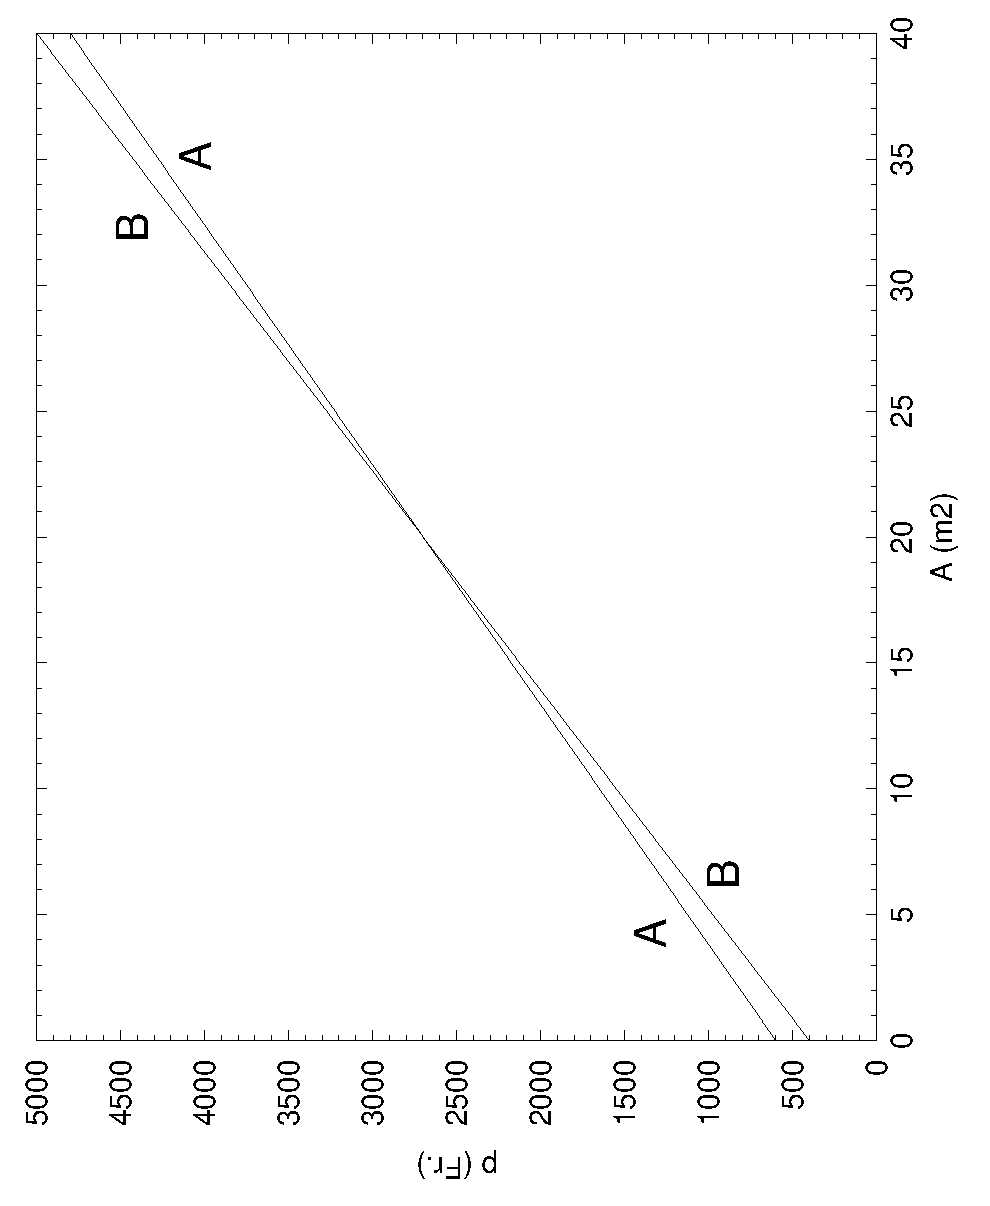
\includegraphics[angle=-90,width=\columnwidth]{pictures/firmen.eps}
      \end{figure}
    \item Aus der Graphik lesen wir ab: Unterhalb von ungef\"ahr $\unit[20]{m^2}$ ist B billiger, oberhalb davon A.

      Algebraisch: F\"ur welche Fl\"ache $A$ ist der Preis gleich: $p_A=p_B=p$?
    \begin{displaymath}
      \left| 
        \begin{array}{rcl}
          p & = & g_A + q_A A \\
          p & = & g_B + q_B A
        \end{array} \right|
    \end{displaymath}
    Gleichsetzungsmethode: Weil der Preis $p$ gleich ist, sind auch die beiden rechten Seiten gleich:
    \begin{eqnarray*}
      g_A + q_A A & = & g_B + q_B A \\
      q_A A - q_B A & = & g_B - g_A \\
      (q_A-q_B)A & = & g_B-g_A \\
      A & = & \frac{g_B-g_A}{q_A-q_B} \\
      A & = & \frac{200\unit{Fr.}}{10\ufrac{Fr.}{m^2}}=20\unit{m^2}
    \end{eqnarray*}
    Die Grenze zwischen den beiden Bereichen liegt tats\"achlich genau bei $\unit[20]{m^2}$. $\result{\mathrm{Unterhalb\;von}\;\unit{m^2}}$ ist B billiger.
    \end{enumerate}

\item 
  \begin{enumerate}
  \item $s$: Distanz von Bern, $t$: Zeit nach 12:00 Uhr, $v_1=90\ufrac{km}{h}$, $v_2=120\ufrac{km}{h}$, $z=144\unit{km}$
    \begin{itemize}
    \item Zug aus Bern: $\result{s=v_1 t}$ oder $\result{s=90\ufrac{km}{h} t}$
    \item Zug aus Z\"urich: $\result{s=z-v_2 t}$ oder $\result{s=z-120\ufrac{km}{h} t}$
    \end{itemize}
    
%\pagebreak
  \item \mbox{}
      \begin{figure}[h]
        \centering
        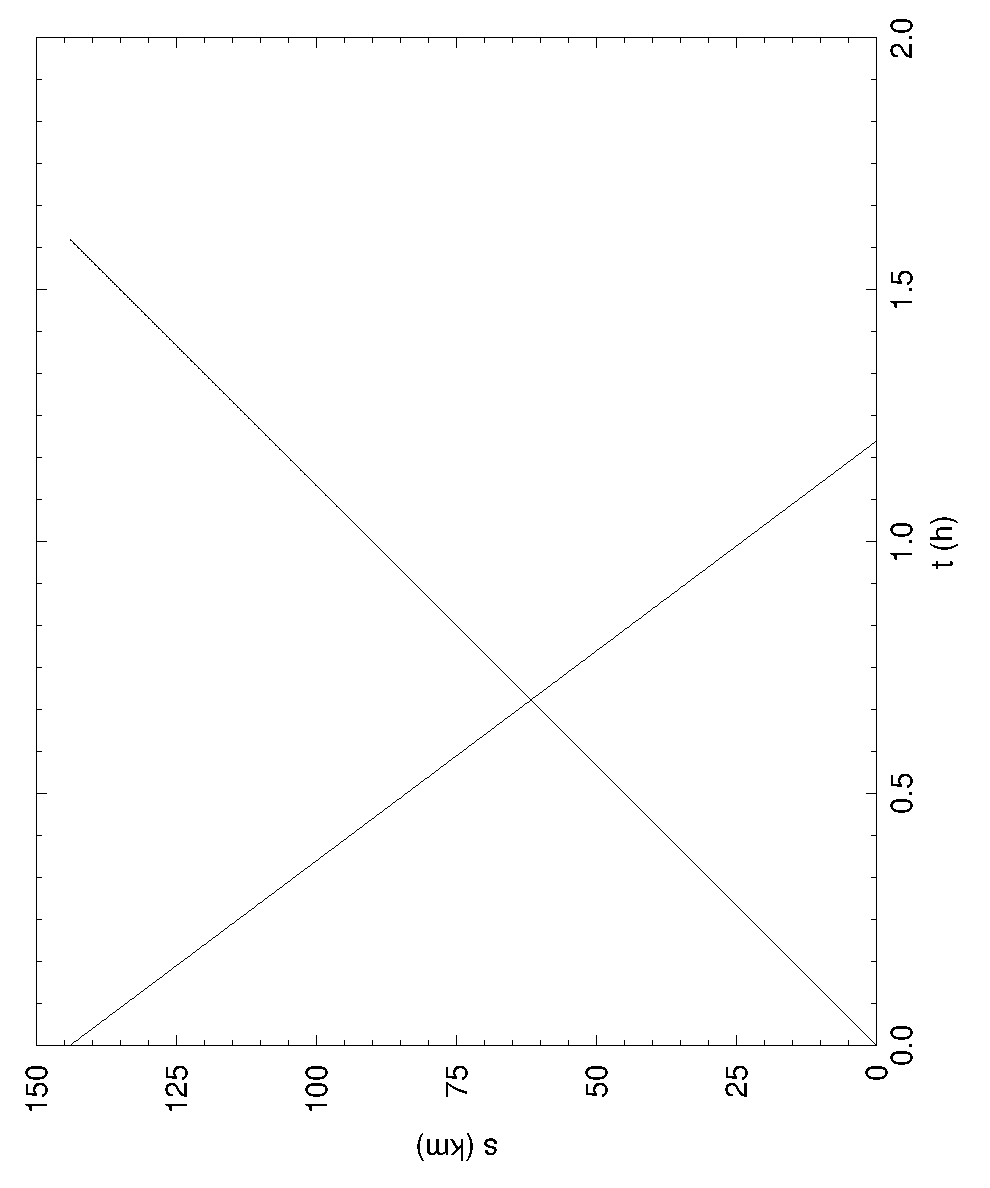
\includegraphics[angle=-90,width=\columnwidth]{pictures/zug.eps}
      \end{figure}
  \item Beide Z\"uge treffen sich, wenn sie zur gleichen Zeit $t$ am gleichen Ort $s$ sind, d.h. im Schnittpunkt der beiden Geraden. Aus dem Weg-Zeit-Diagramm lesen wir heraus, dass das nach gut 40\unit{min} (d.h. um ca. 12:40 Uhr) ungef\"ahr 60\unit{km} von Bern entfernt der Fall ist.

    Algebraisch:
    \begin{displaymath}
      \left| 
        \begin{array}{rcl}
          s & = &  v_1 t \\
          s & = & z-v_2 t
        \end{array} \right|
    \end{displaymath}
    Gleichsetzungsmethode:
    \begin{eqnarray*}
      v_1 t & = & z - v_2 t \\
      v_1 t + v_2 t & = & z \\
      (v_1 + v_2)t & = & z \\
      t & = & \frac{z}{v_1+v_2} \\
      t & = & \frac{144\unit{km}}{210\ufrac{km}{h}}=0.69\unit{h}=41\unit{min}
    \end{eqnarray*}
    Die Z\"uge treffen sich nach $\result{41\unit{min}}$, d.h. 12:41 Uhr. Wir setzen $t$ in die erste Gleichung ein:
    \begin{displaymath}
      s = v_1 t = 90\ufrac{km}{h} \cdot 0.686\unit{h} = 62\unit{km}
    \end{displaymath}
    Die Z\"uge treffen sich $\result{62\unit{km}}$ von Bern entfernt.
  \end{enumerate}


\item
  \begin{enumerate}
  \item 
    \begin{itemize}
    \item $v$: Zahl der Filialen, die vier Mitarbeiter/innen erhalten
    \item $f$: Zahl der Filialen, die f\"unf Mitarbeiter/innen erhalten
    \end{itemize}
    Die Filialen mit 4 Leuten haben zusammen $4v$ Mitarbeiter/innen, jene mit 5 haben $5f$ Angestellte. Zusammen m\"ussen das 57 sein:
    \begin{displaymath}
      4v+5f = 57
    \end{displaymath}
    Insgesamt sind es 12 Filialen:
    \begin{displaymath}
      v+f = 12
    \end{displaymath}
    Beide Bedingungen m\"ussen erf\"ullt sein. D.h. beide Gleichungen bilden zusammen ein Gleichungssystem:
    \begin{displaymath}
      \left| 
        \begin{array}{rcl}
          4v+5f & = & 57 \\
          v+f & = & 12
        \end{array} \right|
    \end{displaymath}
    Einsetzungsverfahren: Wir l\"osen die zweite Gleichung z.B. nach $v$ auf:
    \begin{displaymath}
      \left| 
        \begin{array}{rcl}
          4v+5f & = & 57 \\
          v & = & 12-f
        \end{array} \right|
    \end{displaymath}
    Die zweite Gleichung in die erste einsetzen und nach $f$ aufl\"osen:
    \begin{eqnarray*}
      4(12-f) + 5f & = & 57 \\
      48-4f + 5f & = & 57 \\
      f & = & 9
    \end{eqnarray*}
    $f$ einsetzen in $v=12-f$:
    \begin{displaymath}
      v = 12-f = 3
    \end{displaymath}
    $\result{3}$ Filialen erhalten vier Mitarbeiter/innen und $\result{9}$ erhalten f\"unf. (Diese Aufgabe k\"onnte man auch \"ahnlich l\"osen wie \ref{aufg:linglsystlsg:karten}: Zuerst erh\"alt jede Filiale 4 Leute. Die restlichen 9 Personen werden dann auf entsprechend viele 5er-Filialen verteilt.)

  \item Dachfl\"ache: $A=165\unit{m^2}$, Budget: $B=28500\unit{Fr.}$, Preis Solarpanels: $p_s=242\ufrac{Fr.}{m^2}$, Preis Ziegel: $p_z=105\ufrac{Fr.}{m^2}$

    Gesucht sind die Solarpanel-Fl\"ache $s$ und die Ziegel-Fl\"ache $z$
    \begin{itemize}
    \item Gesamtfl\"ache: $s+z=A$
    \item Kosten der Solarpanels: $p_s s$, Kosten der Ziegel: $p_z z$, zusammen ergibt sich das Gesamtbudget $B$:
      \begin{displaymath}
        p_s s + p_z z = B
      \end{displaymath}
    \end{itemize}
    Beide Gleichungen bilden zusammen ein Gleichungssystem, wobei wir die erste Gleichung bereits nach $s$ aufl\"osen:
    \begin{displaymath}
      \left| 
        \begin{array}{rcl}
          s & = & A-z \\
          p_s s + p_z z & = & B
        \end{array} \right|
    \end{displaymath}
    Einsetzungsverfahren: Wir setzen die erste in die in die zweite Gleichung ein und l\"osen nach $z$ auf:
    \begin{eqnarray*}
      p_s(A-z)+p_z z & = & B \\
      p_s A - p_s z + p_z z & = & B \\
      (p_z-p_s)z & = & B-p_s A \\
      z & = & \frac{B-p_s A}{p_z-p_s} \\
      z & = & \result{83.4\unit{m^2}}
    \end{eqnarray*}
    $z$ in die erste Gleichung einsetzen:
    \begin{displaymath}
      s = A - z = \result{81.6\unit{m^2}}
    \end{displaymath}
  \item $t$: Preis der teuren Bodenplatten, $b$: Preis der billigen Bodenplatten. Eine Gleichunge erhalten wir, indem wir aufschreiben, wie die Gesamtkosten zustande kommen. Die andere dr\"uckt den Preisunterschied aus:
    \begin{displaymath}
      \left| 
        \begin{array}{rcl}
          165t+245b & = & 5929.5\unit{Fr.} \\
          b & = & t - 5\unit{Fr.}
        \end{array} \right|
    \end{displaymath}
    Einsetzungsmethode: Wir setzen die zweite Gleichung in die erste ein und l\"osen nach $t$ auf:
    \begin{eqnarray*}
      165t+245(t-5\unit{Fr.}) & = & 5929.5\unit{Fr.} \\
      165t+245t-1225\unit{Fr.} & = & 5929.5\unit{Fr.} \\
      410t & = & 7154.5\unit{Fr.} \\
      t & = & 17.45\unit{Fr.}
    \end{eqnarray*}
    $t$ in die zweite Gleichung einsetzen:
    \begin{displaymath}
      b = t - 5\unit{Fr.} = 12.45\unit{Fr.}
    \end{displaymath}
  Die Platten kosten pro St\"uck $\result{12.45\unit{Fr.}}$ bzw. $\result{17.45\unit{Fr.}}$


\item $m_1$: Menge Mischung 1, $m_2$: Menge Mischung 2

  Aus den beiden Bedingungen, dass es 10\unit{kg} Klee- und 8\unit{kg} Grassamen sein sollen, ergibt sich je eine Gleichung:
    \begin{displaymath}
      \left| 
        \begin{array}{rcl}
          0.5m_1 + 0.75m_2 & = & 10\unit{kg} \\
          0.5m_1 + 0.25m_2 & = & 8\unit{kg}
        \end{array} \right|
    \end{displaymath}
Gleichsetzungsmethode:
    \begin{displaymath}
      \left| 
        \begin{array}{rcl}
          0.5m_1 & = & 10\unit{kg}-0.75m_2 \\
          0.5m_1 & = & 8\unit{kg}-0.25m_2
        \end{array} \right|
    \end{displaymath}
gleichsetzen:
\begin{eqnarray*}
10\unit{kg}-0.75m_2 & = & 8\unit{kg}-0.25m_2 \\
2\unit{kg} & = & 0.5m_2 \\
4\unit{kg} & = & m_2
\end{eqnarray*}
In eine der obigen Gleichungen einsetzen:
\begin{eqnarray*}
0.5m_1 & = & 8\unit{kg}-0.25m_2 \\
0.5m_1 & = & 8\unit{kg}-0.25\cdot 4\unit{kg} \\
0.5m_1 & = & 7\unit{kg} \\
m_1 & = & 14\unit{kg}
\end{eqnarray*}


\item $a$: Preis Aktive, $g$: Preis G\"aste
    \begin{displaymath}
      \left| 
        \begin{array}{rcl}
          15a + 13g & = & 368\unit{Fr.} \\
          g = a - 4\unit{Fr.}
        \end{array} \right|
    \end{displaymath}
    Zweite Gleichung in erste einsetzen und nach $a$ aufl\"osen:
    \begin{eqnarray*}
      15a+13(a-4\unit{Fr.}) & = & 368\unit{Fr.} \\
      15a + 13a - 52\unit{Fr.} & = & 368\unit{Fr.} \\
      28a & = & 420\unit{Fr.} \\
      a & = & \result{15\unit{Fr.}}
    \end{eqnarray*}
    $a$ einsetzen in die zweite Gleichung:
    \begin{displaymath}
      g = a-4\unit{Fr.} = \result{11\unit{Fr.}}
    \end{displaymath}

\item $v_S$: Geschwindigkeit des Luftschiffs gegen\"uber der Luft. $v_W$: Windgeschwindigkeit.

  Wenn sich das Luftschiff mit $v_S$ gegen\"uber der Luft bewegt und die Luft ihrerseits gegen\"uber der Landschaft mit $v_W$, dann f\"ahrt das Luftschiff gegen\"uber de Erde mit $v_S+v_W$. Das m\"ussen 90.4\ufrac{km}{h} sein:
  \begin{displaymath}
    v_S + v_W = 90.4\ufrac{km}{h}
  \end{displaymath}
  Bei Gegenwind wird die Geschwindigkeit $v_S$ des Luftschiffs hingegen um $v_W$ reduziert:
  \begin{displaymath}
    v_S - v_W = 65.2\ufrac{km}{h}
  \end{displaymath}
  Zusammen bilden die beiden Gleichungen ein Gleichungssystem:
    \begin{displaymath}
      \left| 
        \begin{array}{rcl}
          v_S + v_W & = & 90.4\ufrac{km}{h} \\
          v_S - v_W & = & 65.2\ufrac{km}{h}
        \end{array} \right|
    \end{displaymath}
Gleichsetzungsverfahren:
    \begin{displaymath}
      \left| 
        \begin{array}{rcl}
          v_S & = & 90.4\ufrac{km}{h}-v_W \\
          v_S & = & 65.2\ufrac{km}{h}+v_W
        \end{array} \right|
    \end{displaymath}
gleichsetzen:
\begin{eqnarray*}
90.4\ufrac{km}{h}-v_W & = & 65.2\ufrac{km}{h}+v_W \\
25.2\ufrac{km}{h} & = & 2v_W \\
12.6\ufrac{km}{h} & = & v_W \\
v_S & = & 65.2\ufrac{km}{h}+v_W=77.8\ufrac{km}{h}
\end{eqnarray*}
  \end{enumerate}

\end{enumerate}

\pagebreak

Wir sollten Mathematik auch in konkreten Situationen anwenden k\"onnen. Solche Situationen simulieren die Textaufgaben. Auch wenn sie manchmal etwas k\"unstlich sind, dienen sie uns dazu, an relativ einfachen Beispielen die \"Ubersetzung einer konkreten Situation in die abstrakte Mathematik und wieder zur\"uck zu \"uben. Reale Situationen sind oft komplizierter. Aber wir wollen ja nicht mit dem Kompliziertesten beginnen\dots In diesem Kapitel l\"osen wir die Textaufgaben nach einem Schema mit vier Schritten. Dieses Schema wird an verschiedenen Beispielen erl\"autert. Bei einem Teil der Aufgaben leiten wir die L\"osung als allgemeine Formel her (mit Hilfe von Parametern) und setzen die gegebenen Daten erst am Schluss ein.

\section{Das Monster lässt Grüssen}
\label{lingltext:monster}

Bereits in Kapitel \ref{lingl} (Abschnitt \ref{lingl:lochness}) sind wir von einer Textaufgabe ausgegangen. Dort sind wir nach folgenden Schema vorgegangen:
\begin{enumerate}
\item Was ist gefragt? Die gefragte Gr\"osse benennen wir mit einer Unbekannten. Sie ist die L\"osungsvariable.

$\rightarrow$ $x$: L\"ange des Monsters
\item Welche Aussage macht der Text \"uber diese Gr\"osse? Diese Aussage wird in die algebraische Sprache, d.h. in eine Gleichung \"ubersetzt. Allenfalls muss durch \"Uberlegung eine Gleichheit gefunden werden; z.B. eine Gr\"osse, die in zwei Situationen (z.B. vor- und nachher) gleich ist.

$\rightarrow$ Die L\"ange des Monsters ($x$) ist (=) 20\unit{m} und ($+$) seine halbe L\"ange ($\frac{x}{2}$) lang: 
\begin{displaymath}
  x=20\unit{m}+\frac{x}{2}  
\end{displaymath}

\item Die Gleichung wird nach der L\"osungsvariablen aufgel\"ost.

$\rightarrow$ $x=40\unit{m}$

\item Was bedeutet die L\"osung? Kann sie stimmen? Geh\"ort sie zur Grundmenge der L\"osungsvariablen? (Z.B. darf eine Personenzahl nicht negativ sein.) Evtl. \"uberpr\"ufen wir die L\"osung anhand Textes.

$\rightarrow$ Das Monster ist 40\unit{m} lang. Das kann durchaus sein. Test: Die L\"ange des Monsters, d.h. 40\unit{m}, ist 20\unit{m} und seine halbe L\"ange, d.h. 20\unit{m}, lang. Stimmt!
\end{enumerate}



\clearpage
\listoffigures
%\listoftables
%\newpage
%\nocite{*}
%\bibliographystyle{plain}
%\bibliography{preamble/literaturgoogle}
\end{document}